\documentclass[3p,sort&compress]{elsarticle}
\usepackage{amsfonts,amssymb,amsmath}
\usepackage{graphicx}
\usepackage{bm}
\usepackage{enumerate}
\usepackage{color}

\journal{Physics Reports}

%% `Elsevier LaTeX' style
\bibliographystyle{elsarticle-num}
%%%%%%%%%%%%%%%%%%%%%%%

\begin{document}

\begin{frontmatter}

\title{Complex network approaches to nonlinear time series analysis}

\author[PIK]{Reik V. Donner\corref{corrauthor}}
\cortext[corrauthor]{Corresponding author}
\ead{reik.donner@pik-potsdam.de}
\address[PIK]{Potsdam Institute for Climate Impact Research, P.\,O.~Box
60\,12\,03, 14412 Potsdam, Germany}

\author[ECNU]{Yong Zou\corref{corrauthor}}
\ead{yzou@phy.ecnu.edu.cn}
\address[ECNU]{Department of Physics, East China Normal University, Shanghai 200062, China}

\author[PIK]{Norbert Marwan}
\ead{marwan@pik-potsdam.de}

\author[PIK]{Jonathan F. Donges}
\ead{donges@pik-potsdam.de}

\author[PIK,UK,HU,RU1,RU2]{J\"urgen Kurths}
\ead{kurths@pik-potsdam.de}
 \address[UK]{Institute for Complex Systems and Mathematical Biology, University
 of Aberdeen, Aberdeen AB243UE, United Kingdom}
 \address[HU]{Department of Physics, Humboldt University Berlin,
 Newtonstra{\ss}e 15, 12489 Berlin, Germany}
\address[RU1]{Department of Control Theory, Nizhny Novgorod State University,
Gagarin Avenue 23, 606950 Nizhny Novgorod, Russia} 
\address[RU2]{Institute of Applied Physics of the Russian Academy of Sciences,
603950 Nizhny Novgorod, Russia}


\begin{abstract}

In the last about 10 years, there has been a growing body of literature aiming
at the utilization of complex network methods for the characterization of
dynamical systems based on time series. While both nonlinear time series
analysis and complex network theory are widely considered to be established
fields of complex systems sciences with strong links to Nonlinear Dynamics and
Statistical Physics, the thorough combination of both approaches has become an
active field of research during the last decade, which has allowed addressing
fundamental questions regarding the structural organization of nonlinear
dynamics as well as the successful treatment of a variety of applications from a
broad range of disciplines.

With its three main concepts, phase space / recurrence networks, visibility
graphs and transition / Markov chain networks having made their way from
abstract concepts to widely used methodologies, the field of time series
networks has become mature. These three concepts, as well as several variants
thereof, have been studied in great detail regarding their specific properties,
potentials and limitations and provided fundamental new insights into the
dynamics of complex systems. In addition, these approaches have already found a
wide range of applications from such diverse fields as climatology,
neurophysiology and economics, to mention only a few examples, demonstrating the
great potentials of time series networks to tackling real-world contemporary
scientific problems.

To this end, there exists no thorough overview paper covering all existing
approaches of time series networks. Consequently, we believe that the time is
ripe to deliver such a review covering the methodological foundations,
interpretation and (potential) applications of the existing zoo of methods from
this field. We are confident that Physics Reports would be an excellent forum
for the first review that integrates the state of research on all corresponding
concepts that exist so far.
\end{abstract}

\begin{keyword}
%\MSC[2010] 00-01\sep  99-00
\end{keyword}

\end{frontmatter}
\tableofcontents


%%%%%%%%%%%%%%%%%%%%%%%%%%%%%%%%%%%%%%%%%%%%%%%%%%%%%%%%%%%%%%%%%%%%%%%%%%%%%%%%%%%%%%%
%*****************************CHAPTER/SECTION 1: INTRODUCTION
%%%%%%%%%%%%%%%%%%%%%%%%%%%%%%%%%%%%%%%%%%%%%%%%%%%%%%%%%%%%%%%%%%%%%%%%%%%%%%%%%%%%%%
\section{Introduction {\bf{(Reik+Yong+All)}}}

With the recent increase in available computational capacities and rising data volumes in various fields of science, complex networks have become an interesting and versatile tool for describing structural interdependencies between mutually interacting units \cite{Albert2002,Boccaletti2006,Costa2007,Newman2003}. Besides ``classical'' areas of research (such as sociology, transportation systems, computer sciences, or ecology), where these units are clearly (physically) identifiable, the success story of complex network theory has recently lead to a variety of ``non-conventional'' applications. 

One important class of such non-traditional applications of complex network theory are \emph{functional networks}, where the considered connectivity does not necessarily refer to ``physical'' vertices and edges, but reflects statistical interrelationships between the dynamics exhibited by different parts of the system under study. The term ``functional'' was originally coined in neuroscientific applications, where contemporaneous neuronal activity in different brain areas is often recorded using a set of standardized EEG channels. These data can be used for studying statistical interrelationships between different brain regions when performing certain tasks, having the idea in mind that the functional connectivity reflected by the strongest statistical dependencies can be taken as a proxy for the large-scale anatomic connectivity of different brain regions \cite{Zhou2006,Zhou2007}. Similar approaches have been later utilized for identifying dominant interaction patterns in other multivariate data sets, such as climate data \cite{Donges2009b,Donges2009a,Tsonis2004}.

Besides functional networks derived from multivariate time series, there have been numerous efforts for utilizing complex network approaches for quantifying structural properties of individual time series. In the last decade, several conceptually different approaches have been developed, see \cite{Donner2011IJBC} for a recent review. One important class of approaches make use of ideas from symbolic dynamics and stochastic processes by discretizing the dynamics and then studying the transition probabilities between the obtained groups in some Markov chain-like approach \cite{Nicolis2005}. A second class are visibility graphs and related concepts, which characterize some local convexity or record-breaking property within univariate time series data \cite{Donner2012AG,Lacasa2008,Luque2009}. The latter approach has important applications, such as providing new estimates of the Hurst exponent of fractal and multi-fractal stochastic processes \cite{Lacasa2009,Ni2009} or statistical tests for time series irreversibility \cite{Donges2013EPL,Lacasa2012}. Finally, a third important class of time series networks make use of similarities or proximity relationships between different parts of a dynamical system's trajectory \cite{Donner2011IJBC}, including such diverse approaches as cycle networks \cite{Zhang2006}, correlation networks \cite{Yang2008}, and phase space networks based on a certain definition of nearest neighbors \cite{Xu2008}. One especially important example of proximity networks are recurrence networks (RNs) \cite{Donner2010PRE,Donner2010NJP,Marwan2009}, which provide a reinterpretation of recurrence plots in network-theoretic terms and are already widely applied in a variety of fields.

In this review, we summarize the current state of knowledge on the theoretical foundations and potential applications of recurrence networks. We demonstrate that this type of time series networks naturally arise as random geometric graphs in the phase space of dynamical systems, which determines their structural characteristics and gives rise to a dimensionality interpretation of clustering coefficients and related concepts. In this spirit, the rich toolbox of complex network measures \cite{Boccaletti2006,Costa2007,Newman2003} provides various quantities that can be used for characterizing the system's dynamical complexity from some exclusively geometric viewpoint and allow discriminating between different types of dynamics. Beyond the single-system case, we also provide a corresponding in-depth discussion of cross- and joint recurrence plots from the complex network viewpoint. As a new aspect not previously reported in the literature, we provide a first-time theoretical treatment of a unification of single-system and cross-recurrence plots in a complex network context. Moreover, we discuss some new ideas related to the utilization of multivariate recurrence network-based approaches for studying geometric signatures of coupling and synchronization processes.




\subsection{Nonlinear time series analysis}

A bit more on practical motivation - limitations of existing time series
analysis methods regarding certain common types of problems like detection of
subtle dynamical transitions, time-series reversibility tests, etc.? See comment
of Jonathan (added below at Discussion section)!

\subsection{Complex networks}

\subsection{Transformations from time series to network domain}
\cite{Donner2010NJP,marwan2007}

\subsection{Transformations of complex networks to time series(???)}


\section{Complex network theory {\bf{(Reik, {\color{red}{in Appendix?}})}}}
	\subsection{Basic concepts}

	\subsection{Network characteristics}
 		\subsubsection{Vertex characteristics}
  		\subsubsection{Edge characteristics}
		\subsubsection{Global network characteristics}

	\subsection{Stylized facts of complex networks}
		\subsubsection{Random network models}
		\subsubsection{Scale-free networks}
		\subsubsection{Small-world networks}
		\subsubsection{Assortative mixing}

	\subsection{Coupled networks}
		\subsubsection{General foundations}
		\subsubsection{Vertex characteristics}
		\subsubsection{Global characteristics}
		\subsubsection{Relationships with multi-layer and multiplex networks}


\section{Recurrence networks in phase space {\bf{(Reik)}}} \label{sec:RecurrenceNt}

In this section, we introduce and discuss RNs as an alternative framework for studying recurrences in phase space from a geometric point of view. We start with the basic setting suitable for single dynamical systems, followed by some detailed considerations on two different multivariate generalizations, taking advantage of corresponding recent extensions \cite{Zbilut1998,romano2004} of the recurrence plot (RP) concept \cite{Eckmann1987,marwan2007}. Moreover, we provide a short overview on complex network characteristics and their meaning for RNs, highlighting the type of information that can be obtained using this approach -- as opposed to other recurrence based techniques like recurrence quantification analysis (RQA) \cite{zbilut92,trulla96}, recurrence time statistics, or estimation of dynamical invariants from RPs.


	\subsection{Theoretical background}
\iffalse
% where is the best place to present this table? 
\begin{table}[t]%[H] add [H] placement to break table across pages
\caption{Summary of the definitions of vertices and the criteria for the
existence of edges in existing complex network approaches to time series analysis.}{
%\begin{ruledtabular}
\small
\begin{tabular}{llll}
\hline
Method & Vertex & Edge & Directedness \\
\hline
Proximity networks & & \\
\textit{Cycle networks} & Cycle & Correlation or phase space distance between cycles & undirected \\
\textit{Correlation networks} & State vector & Correlation coefficient between state vectors & undirected \\
\textit{Recurrence networks} & & & \\
\quad \textit{$k$-nearest neighbor networks}& State (vector) & Recurrence of states (fixed neighborhood mass) & directed \\
\quad \textit{adaptive nearest neighbor networks}& State (vector)  & Recurrence of states (fixed number of edges) & undirected \\
\quad \textit{$\varepsilon$-recurrence networks} & State (vector) & Recurrence of states (fixed neighborhood volume) & undirected \\
\hline
Visibility graphs & Scalar state & Mutual visibility of states & undirected \\
\hline
Transition networks & Discrete state & Transitions between states & directed \\
\hline
\end{tabular}
%\end{ruledtabular}
\normalsize
\label{tab:methods}}
\end{table}
\fi

		\subsubsection{Phase space and attractor reconstruction}
		We start with a (possibly multivariate) time series $\{x_i\}_{i=1}^N$ with $x_i=x(t_i)$, which we interpret as a finite representation of the trajectory of some (deterministic or stochastic) dynamical system. For a discrete system (map), the sampling of the time series is directly given by the map, whereas for a continuous-time system, the time series values correspond to a temporally discretized sampling of a finite part of one trajectory of the system determined by some initial conditions. In the case of observation functions not representing the full variety of dynamically relevant components, we additionally assume that attractor reconstruction has been performed reasonable well (e.g., using time-delay embedding or some related technique) \cite{Fraser1986,kantz1997,Kennel1992,Takens1981}. 
		
		More specifically, given a scalar time series $\{x_i\}$ ($i=1,\dots,N$), we first convert the data into state vectors in some appropriately reconstructed phase space. A common method from dynamical systems theory to define such a phase space is time-delay embedding~\cite{Takens1981}. In fact, the concept of a phase space representation rather than a ``simple'' time or frequency domain approach is the hallmark of many methods of nonlinear time series analysis, requiring embedding as the first step. Here, we define $\mathbf{x}_i = (x_i, x_{i-\tau}, \cdots, x_{i-(m-1)\tau})$ to obtain an $m$-dimensional time-delay embedding of $x_i$ with embedding delay $\tau$ for obtaining state vectors in phase space~\cite{Takens1981}. It has been proven that for deterministic dynamical systems, the thus reconstructed phase space is topologically equivalent to the original space if $m > 2 D_F$, where $D_F$ is the fractal dimension of the support of the invariant measure generated by the dynamics in the true (but often at most partially observed) state space. Note that $D_F$ can be much smaller than the dimension of the underlying original (physical) phase space spanned by all relevant system variables. 
		
		From a practical perspective, when analyzing a scalar time series of whatever origin, neither embedding dimension $m$ nor delay $\tau$ are known a priori. The false nearest-neighbors (FNN) method~\cite{Kennel1992} was introduced to derive a reasonable guess of how to choose $m$ based on studying whether or not proximity relations between state vectors are lost when the embedding dimension is successively increased. If a reasonable embedding dimension is found, all dynamically relevant coordinates of the system are appropriately represented, so that all proximity relationships are correct and not due to lower-dimensional projection effects. 
		
		In a similar spirit,  a delay $\tau$ may be appropriate when the auto-covariance approaches zero, i.e., corresponding to the first root of the auto-correlation function (ACF) of a time series. This minimizes the linear correlation between the components but does not have to mean they are independent. However, the converse is true: if two variables are independent they will be uncorrelated. Therefore, another well established possibility for determining $\tau$ is to use time-delayed mutual information \cite{Fraser1986}. 
		
		The aforementioned approaches to determining $m$ and $\tau$ commonly work well for data from deterministic dynamical systems. Let us first assume in the following sections that the proper embeddings have been obtained and then we will discuss the effects of embedding on the reconstructed networks in Sec. \ref{subsec:practicalRN}. This is an important issue when dealing with experimental time series and we have to first check if the appropriate embeddings are applicable. Practically, we need to show the dependence of any analysis on the embeddings explicitly. 
		
		
		\subsubsection{Recurrences and recurrence plots}	
		Recurrence of states, in the meaning that states are arbitrary close after some time, is a fundamental property of deterministic dynamical systems and is typical for nonlinear or chaotic systems \cite{Ott1993,poincare1890}. From the set of (original or reconstructed) state vectors representing a discrete sampling of the underlying system's trajectory (e.g., the chaotic attractor of a dissipative system), recurrences can be visualized by recurrence plots (RP), introduced by Eckmann {\textit{et al.}} in \cite{Eckmann1987,marwan2007} and the RP is represented by the recurrence matrix $\textbf{R}(\varepsilon)$ in the standard way as
\begin{equation}
R_{ij}(\varepsilon)=\Theta(\varepsilon-\|x_i-x_j\|),
\end{equation}
\noindent
where $\|\cdot\|$ can be any norm in phase space (e.g., Manhattan, Euclidean, or maximum norm). For convenience, we will use the maximum norm in all following examples. A RP enables us to investigate the recurrences of the $m$-dimensional phase space trajectory through a two-dimensional representation $R_{ij}$ with dots. 

The basic principle is illustrated in Fig.~\ref{lorenz_constr} for one realization of the Lorenz system 
\begin{equation}
\frac{d}{dt}\left(\begin{array}{c}x\\y\\z\end{array}\right)=\left(\begin{array}{c}\sigma(y-x) \\ x(r-y)\\ xy-\beta z \end{array}\right).
\label{eq_lorenz}
\end{equation}
\noindent
Further definitions of recurrences add dynamical aspects, such as local rank orders or strictly parallel evolution of states (parallel segments of phase-space trajectory considered in iso-directional RPs~\cite{Horai2002}). For a more detailed overview, we refer to~\cite{marwan2007}.
\begin{figure}[thb]
	\centering
	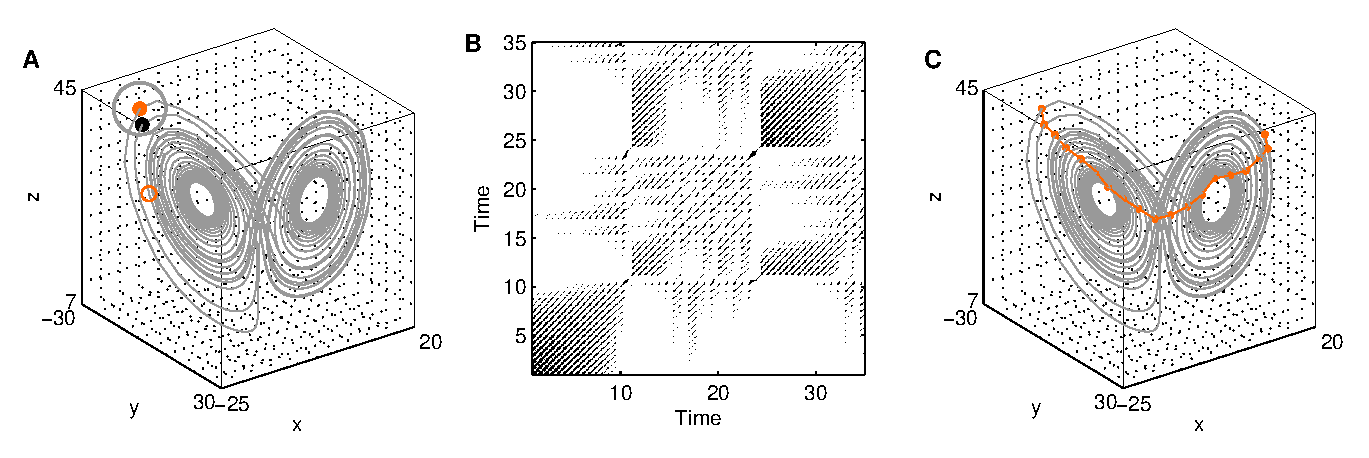
\includegraphics[width=\textwidth]{Chapter03_RecurrenceNt/lorenz_constr.eps}
	% 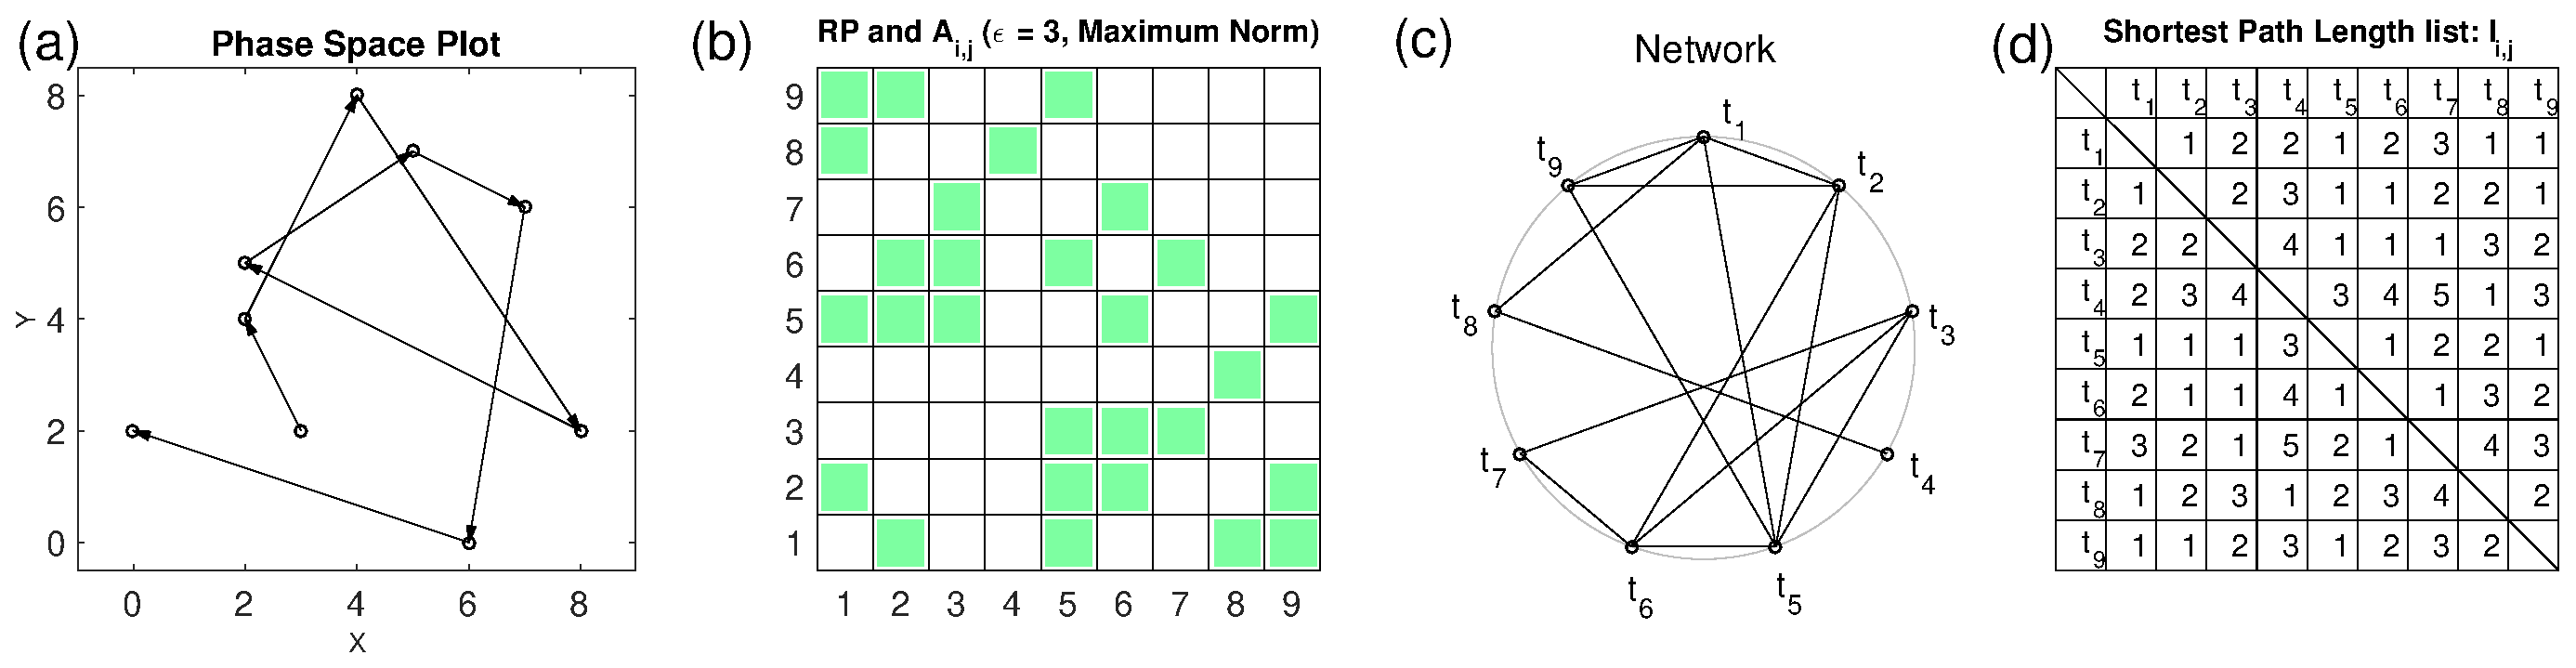
\includegraphics[width=\textwidth]{Chapter03_RecurrenceNt/toy_modelPR.eps}
\caption{Basic concepts beyond recurrence plots and the resulting recurrence networks, exemplified for one realization of the Lorenz system (Eq.~(\ref{eq_lorenz})) with the parameters $r=28$, $\sigma=10$ and $\beta=8/3$ (sampling time $\Delta t=0.02$, original coordinates, no embedding, recurrences defined based on a fixed threshold $\varepsilon=5.0$ using maximum norm). (A) A state at time $i$ (red dot) is recurrent at another time $j$ (black dot) when the phase space trajectory visits its close neighborhood (gray circle). This is marked by value 1 in the recurrence matrix at $(i,j)$. States outside of this neighborhood (small red circle) are marked with 0 in the recurrence matrix. (B) Graphical representation of the corresponding recurrence matrix (recurrence plot) and adjacency matrix (modulo main diagonal). (C) A particular path in the recurrence network for the same system embedded in the corresponding phase space. Reproduced from \cite{Donner2011}. {\color{red} We need to put panel (C) into Fig. \ref{lorenz_net}(b). }}
\label{lorenz_constr}
\end{figure}

RPs of dynamical systems with different types of dynamics exhibit distinct structural properties, which can be characterized in terms of their associated small-scale as well as large-scale features~\cite{marwan2007}. The study of recurrences by means of RPs has become popular with the introduction of recurrence quantification analysis (RQA)~\cite{zbilut92,marwan2002}. The initial purpose of this framework has been to introduce measures of complexity which distinguish between different appearances of RPs~\cite{marwan2008}, since they are linked to certain dynamical properties of the studied system. RQA measures use the distribution of small-scale features in the RP, namely individual recurrence points as well as diagonal and vertical line structures. RQA as a whole has been proven to constitute a very powerful technique for quantifying differences in the dynamics of complex systems and has meanwhile found numerous applications, \textit{e.g.,} in ecology \cite{facchini2007}, engineering \cite{litak2009c}, geo- and life sciences \cite{marwan2003climdyn,marwan2007pla}, or protein research \cite{Giuliani2002a,zbilut2004a}. For a more comprehensive review on the potentials of this method, we refer to \cite{marwan2008epjst,webber2009}. In addition, we would like to remark that even dynamical invariants, like the $K_2$ entropy and mutual information, or dimensions (information and correlation dimensions $D_1$, $D_2$) can be efficiently estimated from RPs \cite{thiel2004a,marwan2007}. Moreover, RPs have also been successfully applied to study interrelations, couplings, and phase synchronization between dynamical systems~\cite{marwan2002npg,romano2004,romano2005,Romano2007,vanLeeuwen2009,Nawrath2010}.

In order to highlight the domains of recurrences in the RPs, some sophisticate algorithms have been proposed recently. For example, Pham {\textit {et al}} introduced fuzzy recurrence plots, which determines an optimally relation of the phase space states to a number of predefined clusters \cite{Pham2016}. This algorithm highlights the recurrence regions giving better visualizations. Recently another algorithm has been proposed to search the recurrence domains in \cite{graben2013}. In particular, intersecting $\varepsilon$-balls around sampling points are merged into cells of a phase space partition and a maximum entropy principle defines the optimal size of intersecting balls. This adaptive algorithm in obtaining phase partitions performs better than techniques based on Markov chains which require an ad hoc partition of the system's phase space. In the same line of research, another algorithm has been proposed in \cite{Costa2018} to capture the recurrence density structures in the plot. The computation complexity of RQA measures has been recently evaluated \cite{Martinovic2018}. 


		% \subsubsection{Related approaches to time series analysis}

	\subsection{Types of recurrence networks}
		\subsubsection{$\varepsilon$-recurrence networks}
		We can re-interpret the mathematical structure $\textbf{R}(\varepsilon)$ as the adjacency matrix of some adjoint complex network embedded in phase space by setting
\begin{equation}
\mathbf{A}(\varepsilon)=\mathbf{R}(\varepsilon)-\mathbf{1}_N,
\label{eq:rn_definition}
\end{equation}
\noindent
where $\mathbf{1}_N$ is the $N$-dimensional identity matrix. The complex network defined this way is called \emph{$\varepsilon$-recurrence network (RN)}, as opposed to other types of proximity-based networks in phase space making use of different definitions of geometric closeness, e.g., considering $k$-nearest neighbors~\cite{Donner2011}. Specifically, the sampled state vectors $\{x_i\}$ are interpreted as vertices of a complex network, which are connected by undirected edges if they are mutually close in phase space (i.e., describe recurrences). Notably, the binary matrix $\mathbf{A}(\varepsilon)$ retains the symmetry properties of $\mathbf{R}(\varepsilon)$, which implies that the RN is a \emph{simple graph}, i.e., a complex network without multiple edges or self-loops (note that $A_{ii}=0$ according to definition~(\ref{eq:rn_definition})). We show an example of an unweighted  $\varepsilon$-RN network in \ref{lorenz_net}. 
\begin{figure}[thb]
	\centering
	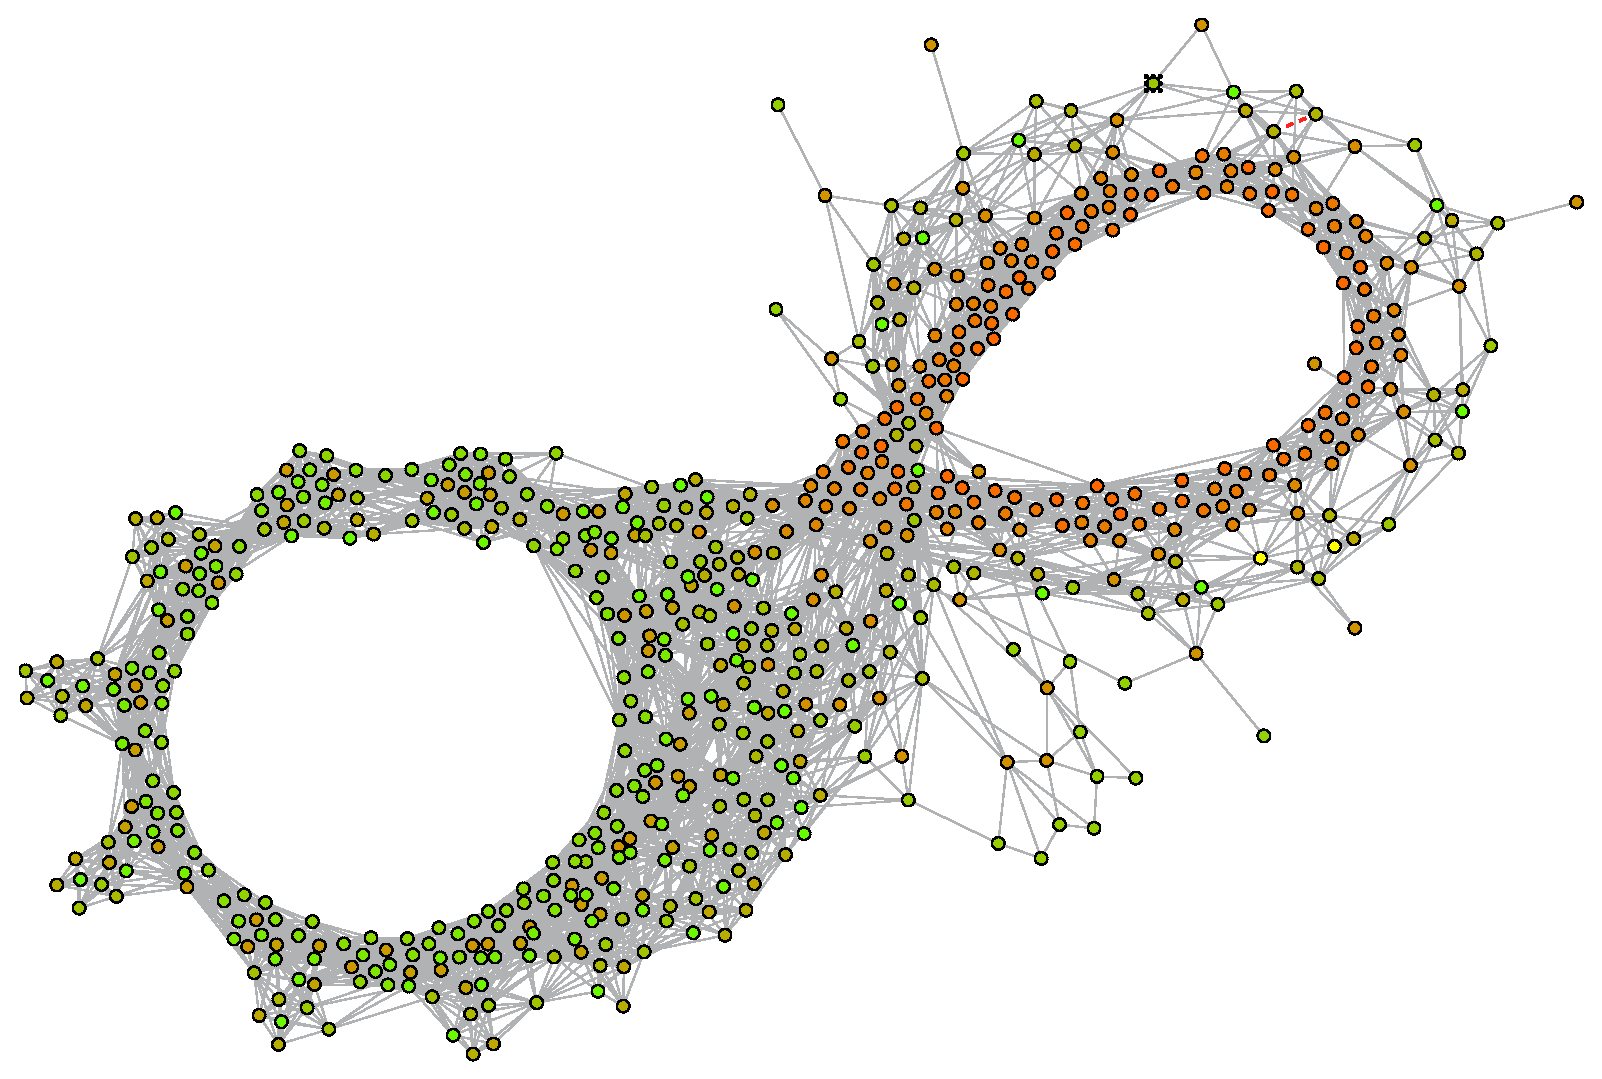
\includegraphics[width=0.48\textwidth]{Chapter03_RecurrenceNt/lorenz_net.eps}
\caption{(A) A graphical representation of the Lorenz attractor based on the recurrence matrix represented in Fig.~\ref{lorenz_constr}. The color of the vertices corresponds to their temporal order (from orange to bright green). (B) A particular path in the RN for the same system embedded in the corresponding phase space. Reproduced from \cite{Donner2011}. {\color{red}We need Fig. \ref{lorenz_constr}(C) here. }}
\label{lorenz_net}
\end{figure}

		In an $\varepsilon$-RN, a \emph{path} between two specified vertices $i$ and $j$ is an ordered sequence of edges starting at $i$ and ending at $j$, with its \emph{path length} $d_{ij}(\varepsilon)$ given by the number of edges in this sequence. An example of a path is shown in Fig. \ref{lorenz_net}. In the context of RNs, we can thus understand a path as a sequence of mutually overlapping $\varepsilon$-balls\footnote{Here, $\varepsilon$-balls refers to general (hyper-)volumes according to the specific norm chosen for measuring distances in phase space, e.g., hypercubes of edge length $2\varepsilon$ in case of the maximum norm, or hyperballs of radius $\varepsilon$ for the Euclidean norm.} $B_{\varepsilon}(x_i),B_{\varepsilon}(x_{k_1}),\dots,B_{\varepsilon}(x_{k_{l_{i,j}-1}}),B_{\varepsilon}(x_j)$, where $$B_{\varepsilon}(x)=\{y\,|\,\|x-y\|<\varepsilon\}$$ is an open set describing a volume with maximum distance $\varepsilon$ (measured in a given norm) from $x$, and $B_{\varepsilon}(x_i)\cap B_{\varepsilon}(x_{k_1})\neq\emptyset,\dots,B_{\varepsilon}(x_{k_{l_{i,j}-1}})\cap B_{\varepsilon}(x_j)\neq\emptyset$.
		
		Following these considerations, a \emph{shortest path} is a minimum sequence of edges (mutually overlapping $\varepsilon$-balls) between two fixed vertices (state vectors) $i$ and $j$. Note that a shortest path does not need to be unique. In turn, due to the discrete character of a network, it is rather typical that there are multiple shortest paths between some specific pair of vertices. In what follows, the shortest path length will be denoted as ${d}_{ij}$, and the multiplicity of such shortest paths as ${\sigma}_{ij}$.
		
		We have to emphasize that the network-theoretic concept of a path on a given graph is distinctively different from the trajectory concept that records the causal dynamic evolution of the system \cite{Donner2010a}. Furthermore, RNs based on Eq.~(\ref{eq:rn_definition}) can be generalized by withdrawing the application of a specific threshold, which leads to weighted networks and unthresholded RPs (distance plots), respectively. For example, the unthresholded RP obtained from one trajectory of a given dynamical system may be re-interpreted as the connectivity matrix of a fully coupled, weighted network. 
		
	 	Most of RN analysis have focused on the network representation using the adjacency matrix and the extraction of new network-theoretic measures, which will be reviewed below. We have to emphasize that the adjacency matrix provides information of vertices and edges, but its graph structural layouts can take variable forms.  Network visualization is a non-trivial task and there are many tools in computer science, for example, spring-based layout systems, spectral layout method, and tree layout algorithms etc. These algorithms have been well integrated in many popular network visualization packages, i.e., Mathematica, Gephi, and NetworkX. The network graph shown Fig. \ref{lorenz_net} has been created using the software package {\tt{GUESS}} using a force directed placement algorithm. In \cite{Yang2013}, Yang {\textit{et al}} proposed to use the spring-electrical model to explore the self-organized geometry of RNs. In this algorithm, they simulate the recurrence network as a physical system by treating the edges as springs and the nodes as electrically charged particles. Then, force-directed algorithms are developed to automatically organize the network geometry by minimizing the system energy. It has been shown that this self-organized process recovers the attractor of a dynamical system, which provides insights for attractor reconstruction from the adjacency matrix \cite{thiel2004b,hirata2008}. 
			
	
		\subsubsection{$k$-nearest neighbor networks}
		Besides the recurrence definition based on a fixed distance threshold $\varepsilon$ in phase space (i.e., equal neighborhood volumes around all available state vectors), there are alternative ways for defining recurrences and, hence, RPs and RNs. For example, the original definition of a RP by Eckmann \textit{et~al.} \cite{Eckmann1987} makes use of $k$-nearest neighbors (i.e., a fixed probability mass of the considered neighborhoods). Re-interpreting the resulting recurrence matrix as the adjacency matrix of a complex network leads to a different type of RN \cite{Shimada2008}, typically referred to as \emph{$k$-nearest neighbor network}. Since in this definition, the neighborhood relation is not symmetric (i.e., $x_j$ being among the $k$ nearest neighbors of $x_i$ does not imply $x_i$ also being among the $k$ nearest neighbors of $x_j$), the resulting networks are in general directed graphs, and the local density of unidirectional edges (as opposed to bidirectional ones) is related to the gradient of the invariant density.
		
		\subsubsection{Adaptive neighbor networks}
		In order to circumvent the directedness of $k$-nearest neighbor networks, Xu \textit{et~al.} \cite{Small2009,Xu2008} proposed an algorithm for balancing the neighborhood relationships in such a way that they become symmetric again. The resulting networks embedded in phase space, sometimes also referred to as \emph{adaptive nearest neighbor networks} \cite{Donner2011}, are conceptually more similar to classical ($\varepsilon$-)RNs, but still exhibit somewhat different topological characteristics. In particular, this approach helps to understand the superfamily phenomena of time series, which concern the relative prevalence of motifs of the resulting networks. In particular, the motif distribution of adaptive nearest neighbor networks has been empirically shown to allow a discrimination between different types of dynamics in terms of a different motif ranking \cite{Xu2008}. Consequently, this approach has been mainly used for such discriminatory tasks, including applications to turbulence phenomena, instrumental music \cite{Donner2011}, fractional Brownian motions and multifractal random walks \cite{Liu2010a}. 
		
		While these superfamily phenomena have been found in time series from various origins, no concrete theories have been proposed in the literature. Khol {\textit{et al}} provides a heuristic explanation of superfamily phenomena by examining the dependence of attractor dimension on motif prevalence \cite{Khor2016}. Since the reconstructed networks inherently capture the proximity of states, motifs represent specific arrangements of states in space, some of which are more or less likely to occur as dimension changes. Therefore, they found that the relative prevalence of motifs are strongly dependent on the local dimension of the space from which the state vectors are taken. Further evidence is given by identifying comparable superfamily phenomena in networks constructed from states randomly distributed in spaces of varying dimensions \cite{Khor2016}.

		\subsubsection{Algorithm comparisons and variants}
		For a detailed discussion of the differences between $\varepsilon$-RNs, $k$-nearest neighbor and adaptive nearest neighbor networks, we refer to \cite{Donner2011}. While these three classes of time series networks exhibit very strong conceptual similarities (the same applies to correlation networks \cite{Yang2008} if interpreting the correlation coefficient between two sufficiently high-dimensional state vectors as a generalized distance), the approach proposed by Li \textit{et~al.} \cite{Li2011a,Li2011b,Cao2014,Fan2015} can be understood as being derived from the RN idea. Here, for a set of $m$-dimensional embedding vectors, all mutual Euclidean distances are computed. Based on the maximum point-wise Euclidean distance $d_{max}(m)$, the threshold distance of an RN is taken as $\varepsilon(m)=d_{max}(m)/(N-1)$. This procedure is repeated for different $m$, and the critical value of the embedding dimension for which the resulting network gets completely disconnected is interpreted as a complexity index \cite{Cao2014}. However, it has not yet been demonstrated that this algorithmic approach has any conceptual benefits in comparison with the classical RN transitivity obtained for a fixed embedding dimension.

		Another conceptual approach loosely related to RNs provides the foundation of the frequency-degree mapping algorithm introduced by Li \textit{et~al.} \cite{Li2012}. Here, the resulting time series networks contain two types of edges: (i) temporal edges connecting subsequent points in time, and (ii) proximity edges containing observations of similar values, where similarity is defined by an initial grouping of the data into a discrete set of classes, and observed values being connected if and only if they belong to the same class. Here the definition of a class is equivalent to a recurrence interval that is defined by amplitude quantization, for instance, the recurrence interval length $I = H/Q$ where $Q$ is the quantization level and $H$ is the amplitude range of time series. Notably, the latter approach combines the classical recurrence idea and basic concepts of symbolic dynamics \cite{Daw2003}. In this spirit, the resulting network's adjacency matrix is given as the recurrence matrix associated with a symbolic recurrence plot \cite{Donner2008,Faure2010,graben2013} plus a ``stripe'' around the matrix' main diagonal. The frequency-degree mapping algorithm has been successfully applied to characterizing signatures of various types of ventricular arrhytmias in human heart beat time series \cite{Li2012}, stock markets \cite{Cao2014}, and air quality indices \cite{Fan2015}.

		In order to highlight the recurrence domains in the networks, fuzzy recurrence network approach has been proposed in \cite{Pham2017}, which shares much similarities with fuzzy recurrence plots \cite{Pham2016}. Furthermore, a grammatical rewriting algorithm over the recurrence matrix has been proposed to search for recurrence domains in \cite{graben2013}, which presents a symbolic description of recurrence properties of time series. It is interesting to see that this algorithm yields an optimal symbolic recurrence representation revealing functional components of brain signals \cite{graben2013}. Note that the computation of recurrence matrix is the first step of this grammatical algorithm. 

		The computation time of a RN is proportional to $N^2$ where $N$ is the number of time points, which calls for more efficient algorithm in constructing RNs for long time series. In the case of long time series, on the other hand, we are more interested in the evolution behavior of RN over time. To this end, sliding window techniques are often suggested but we need to check the dependence on the choice of window sizes \cite{Donges2011a,Donges2011}. Another idea is to perform coarse graining of the original RNs \cite{Costa2018}, which stems from original idea of meta recurrence plots \cite{casdagli97}. In \cite{Iwayama2012}, the authors proposed to first divide the original long time series into short segments and RNs are reconstructed for each piece. The next step is to build joint recurrence networks for each pair of windowed segments. Then, the global overview of the long term dynamics is characterized by the variations of the network properties that are computed for meta-time series. 


		\subsection{Complex network characteristics of RN}\label{sec:rn_measures}
		Based on the re-interpretation of the recurrence matrix $\mathbf{R}(\varepsilon)$ as the adjacency matrix of an adjoint RN, we can utilize the large toolbox of complex network measures~\cite{Albert2002,Boccaletti2006,Costa2007,Newman2003} for characterizing the structural organization of a dynamical system in its phase space. Notably, this viewpoint is complementary to other concepts of nonlinear time series analysis making use of RPs. For example, RQA characterizes the statistical properties of line structures in the RP, which implies explicit consideration of dynamical aspects (i.e., sequences of state vectors) \cite{marwan2007}. In turn, RNs do not make use of time information, since network properties are generally invariant under vertex relabelling (i.e., permutations of the order of observations) \cite{Donner2010a}. In this spirit, RN analysis provides geometric instead of dynamical characteristics. This idea of a geometric analysis is similar to some classical concepts of fractal dimensions (e.g., box-counting or correlation dimensions), where certain scaling laws in dependence on the spatial scale of resolution (corresponding here to $\varepsilon$) are exploited. In turn, RN analysis can be performed (as RQA) using only a single fixed scale ($\varepsilon$) instead of explicitly studying scaling properties over a range of threshold values.

		The distinction between dynamical and geometric information implies that in case of RN analysis, the typical requirement of a reasonable (typically uniform) temporal sampling of the considered trajectory is replaced by the demand for a suitable spatial coverage of the system's attractor in phase space. Specifically, under certain conditions the latter could also be obtained by considering an ensemble of short trajectories instead of a single long one. If the trajectory under study is relatively densely sampled, trivial serial correlations can lead to a selection bias in the set of sampled state vectors; the latter could be avoided by reasonable downsampling. In the same context, the possibility of utilizing Theiler windows for removing edges representing short-term auto-correlations (e.g., recurrence points close to the main diagonal in the RP) should be mentioned as another strategy based on a somewhat different rationale~\cite{Donner2010a}. However, from a conceptual perspective, downsampling can provide an unbiased sampling of the attractor as long as the fixed sampling time does not correspond to any integer multiple of some of the system's natural frequencies. As an alternative, bootstrapping from the set of available state vectors provides another feasible option, which should be preferred if a sufficiently long time series is available. In general, numerical experiments and different applications suggest that stable estimates of RN characteristics can often already be obtained using a sample size of $N\sim\mathcal{O}(10^2\dots 10^3)$ data points~\cite{Donges2011,Donges2011a}.

		In Sec. \ref{sec:basictheoryCN}, we have provided a general review on various network measures characterizing the structural properties of a complex network as denoted by the adjacency matrix $A$. In this section, we further discuss the physical interpretations of these measures in terms of phase space properties as captured by RN representations. In what follows, we will denote all properties computed from a RN consisting of a finite number $N$ of state vectors as $\hat{f}$, pointing to the fact that they are estimated from a given sample of state vectors but shall characterize the entire trajectory of the system under study. Namely, we have specific finite estimations for Eqs. \eqref{eq:degree}-\eqref{eq:apl}. Furthermore, we will discuss a corresponding continuous framework generalizing all network characteristics described below in Section \ref{sec:analyticRNtheory}. In order to focus the following discussion, we review only the possibly most relevant characteristics associated with RNs. More details including further measures can be found in \cite{Donges2012,Donner2010a}.
		
		When considering quantitative characteristics of complex networks, different classifications of measures are possible. First, we may distinguish measures based on the concept of graph neighborhoods from those making use of shortest path-based characteristics. (This is not an exhaustive classification, since it potentially neglects other important network measures, e.g., such based on diffusion processes or random walks on the network.) Second, network measures can be classified into such making use of local, meso-scale and global information. This scheme is widely equivalent to the first one in that local information refers to properties determined by the graph neighborhood of a given vertex, whereas global information takes contributions due to all vertices of the network into account, which is common for shortest path-based measures. Finally, we can differentiate between measures quantifying properties of single vertices, pairs of vertices, and the network as a whole. In this chapter, we will utilize the latter way of classification, since it appears most instructive from the applied point of view (i.e., we are commonly interested in either the local or the global geometry of an attractor).
			
				\subsubsection{Vertex characteristics}
        				The network \textit{degree} or \textit{degree centrality} of a single vertex $x_v$ (Eq. \eqref{eq:degree}) has 
\begin{equation}
\hat{k}_v(\varepsilon)=\sum_{i=1}^N A_{iv}(\varepsilon). 
\label{eq:degree}
\end{equation}
% which simply counts the number of edges associated with a given vertex $v$. 
 From the perspective of recurrences, it is reasonable to replace the degree by a normalized characteristic, the \textit{degree density}
\begin{equation}
\hat{\rho}_v(\varepsilon)=\frac{\hat{k}_v(\varepsilon)}{N-1}=\frac{1}{N-1} \sum_{i=1}^N A_{iv}(\varepsilon),
\label{eq:locrho}
\end{equation}
\noindent
which corresponds to the definition of the local recurrence rate of the state $x_v$. $\hat{\rho}_v(\varepsilon)$ quantifies the density of states in the $\varepsilon$-ball around $x_v$, i.e., the probability that a randomly chosen member of the available sample of state vectors is $\varepsilon$-close to $x_v$. An illustration of this fact for the Lorenz system is presented in Fig.~\ref{fig:local}(a); here, phase space regions with a high density of points (i.e., a high residence probability of the sampled trajectory) are characterized by a high degree density.
\begin{figure}
	\centering
	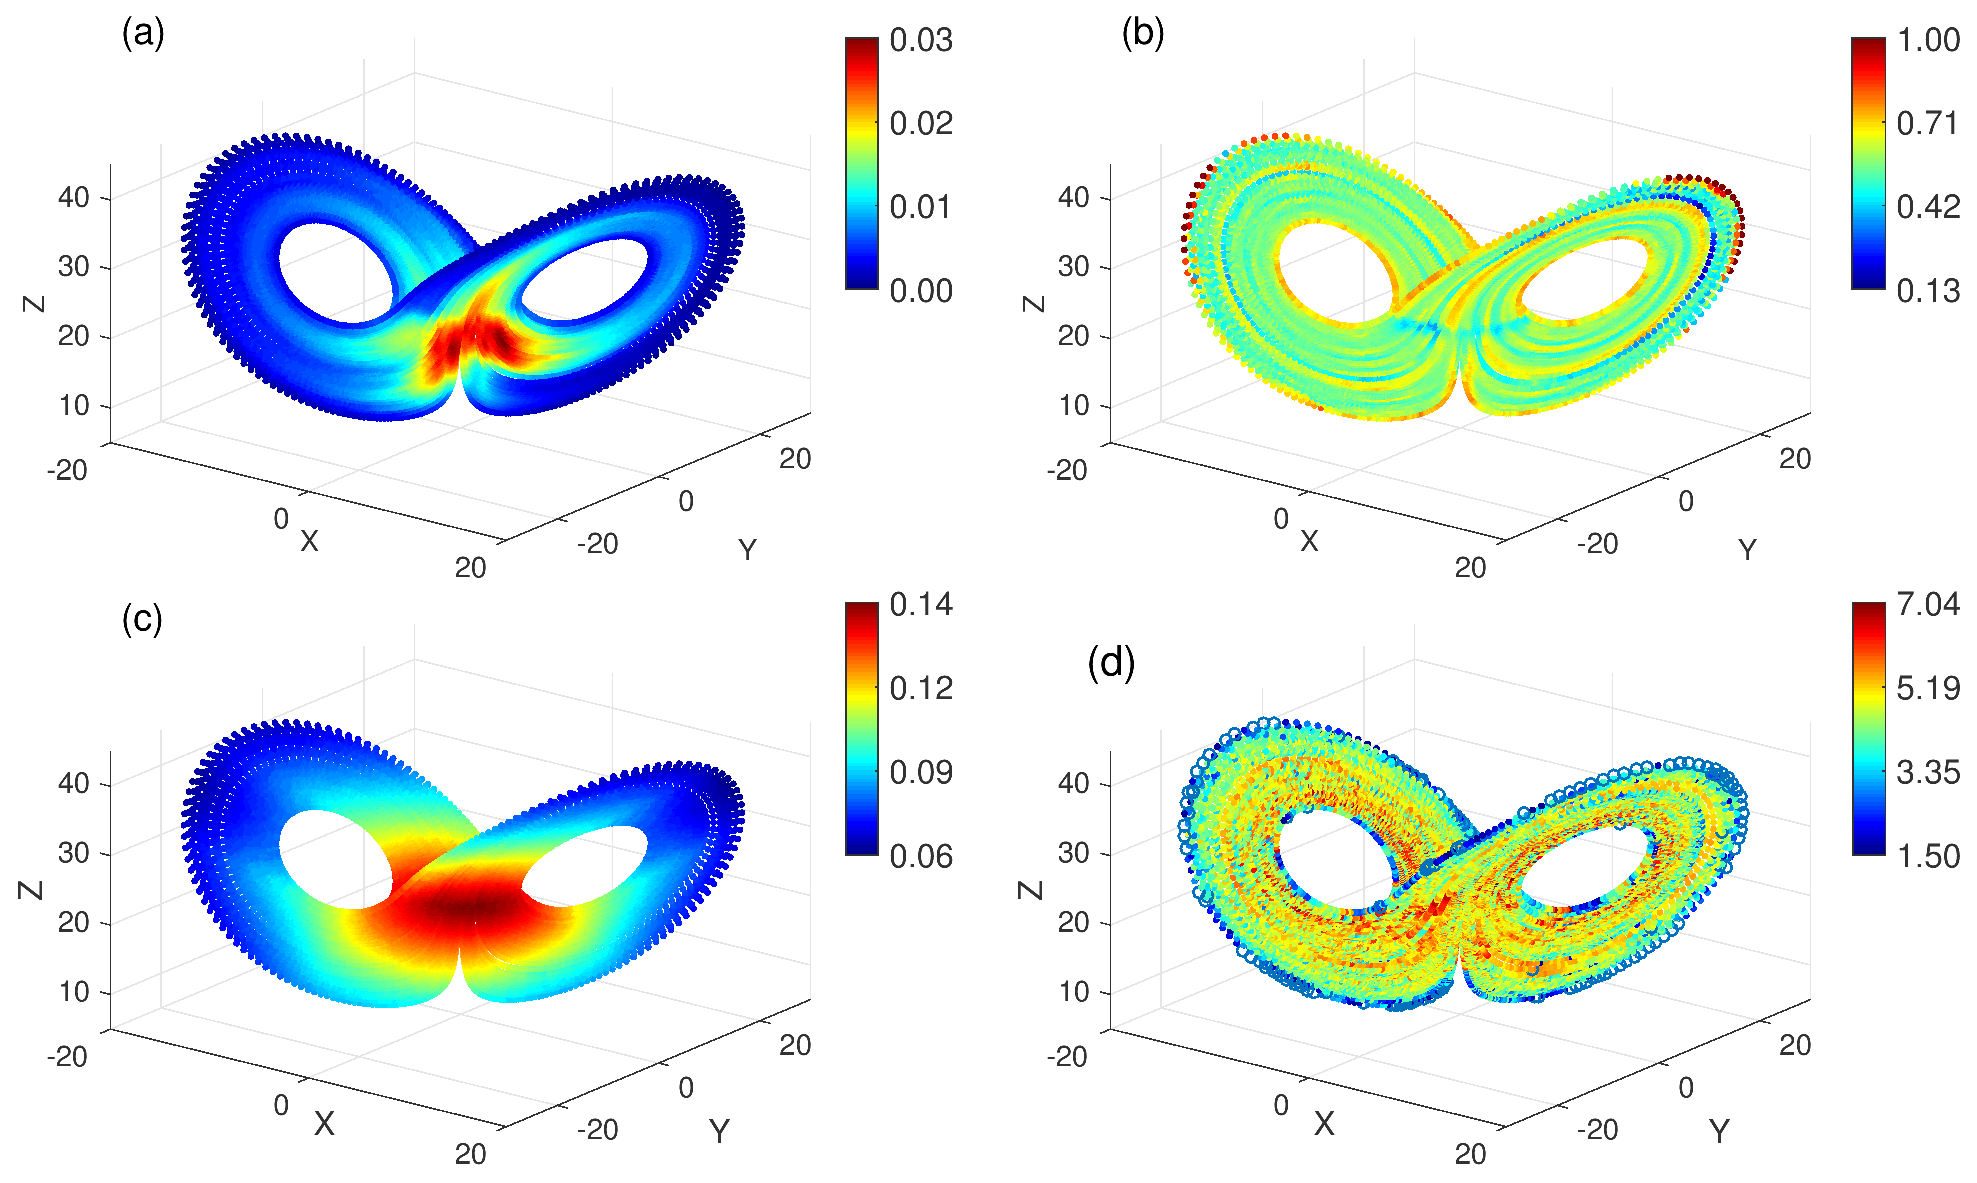
\includegraphics[width=\columnwidth]{Chapter03_RecurrenceNt/phase_deg_cc_cls_btwLoenz.eps}
\caption{Spatial distributions of vertex characteristics of the $\varepsilon$-RN obtained for the Lorenz system (Eq.~\ref{eq_lorenz}) at the canonical parameters (RPs computed using the maximum norm with $\hat{\rho}=0.01$, $N=20,000$ and sampling time $\Delta t=0.1$): (a) $\hat{k}_v(\varepsilon)$, (b) $\hat{\mathcal{C}}_v(\varepsilon)$, (c) $\hat{c}_v(\varepsilon)$, (d) $\hat{b}_v(\varepsilon)$. Reproduced from \cite{Donner2010a}. } \label{fig:local}
\end{figure}

% In order to characterize the density of connections among the neighbors of a given vertex $v$, we can utilize the \textit{local clustering coefficient}
The \textit{local clustering coefficient} (Eq. \eqref{eq:locclustering}) reads
\begin{equation}
\hat{\mathcal{C}}_v(\varepsilon)=\frac{1}{\hat{k}_v(\varepsilon)(\hat{k}_v(\varepsilon)-1)} \sum_{i,j=1}^N A_{vi}(\varepsilon) A_{ij}(\varepsilon) A_{jv}(\varepsilon),
\label{eq:locclusteringRN}
\end{equation}
\noindent
which measures the fraction of pairs of vertices in the $\varepsilon$-ball around $x_v$ that are mutually $\varepsilon$-close. For vertices with $\hat{k}_v(\varepsilon)<2$, we define $\hat{\mathcal{C}}_v(\varepsilon)=0$. It has been shown that the local clustering coefficient in a RN is associated with the geometric alignment of state vectors. Specifically, close to dynamically invariant objects such as unstable periodic orbits (UPOs) of low period, the dynamics of the system is effectively lower-dimensional, which results in a locally enhanced fraction of closed paths of length 3 (``triangles'') and, thus, a higher local clustering coefficicent. The latter behavior is exemplified in Fig.~\ref{fig:local}(b) for the Lorenz system, where we recognize certain bands with higher values of $\hat{\mathcal{C}}_v$ corresponding to the positions of known low-periodic UPOs~\cite{Donner2010a}.

% While degree and local clustering coefficient characterize network structures on the local and meso-scale, there are further vertex characteristics that make explicit use of the concept of shortest paths and, thus, provide measures relying on the connectivity of the entire network. Two specific properties of this kind are 
The \textit{closeness} or \textit{closeness centrality} (Eq. \eqref{eq:closeness}) reads 
\begin{equation}
\hat{c}_v(\varepsilon)=\left(\frac{1}{N-1}\sum_{i=1}^N \hat{d}_{vi}(\varepsilon) \right)^{-1},
\label{eq:closenessRN}
\end{equation}
\noindent
% which gives the inverse arithmetic mean of the shortest path lengths between vertex $v$ and all other vertices, 
and the \textit{local efficiency} (Eq. \eqref{eq:locefficiency}) is 
\begin{equation}
\hat{e}_v(\varepsilon)=\frac{1}{N-1}\sum_{i=1}^N \hat{d}_{vi}(\varepsilon)^{-1}. 
\label{eq:locefficiencyRN}
\end{equation}
\noindent
% which gives the inverse harmonic mean of these shortest path lengths. Notably, the latter quantity has the advantage of being well-behaved in the case of disconnected network components, where there are no paths between certain pairs of vertices (i.e., $\hat{d}_{ij}=\infty$). In order to circumvent divergences of the closeness due to the existence of disconnected components, it is convenient to always set $\hat{d}_{ij}$ to the highest possible value of $N-1$ for pairs of vertices that cannot be mutually reached. Both $\hat{c}_v(\varepsilon)$ and $\hat{e}_v(\varepsilon)$ characterize the geometric centrality of vertex $v$ in the network, i.e., closeness and local efficiency exhibit the highest values for such vertices which are situated in the center of the RN (see Fig.~\ref{fig:local}C for an illustration for the R\"ossler system).
Here again, we set $\hat{d}_{ij}$ to the highest possible value of $N-1$ for pairs of vertices that cannot be mutually reached. Both $\hat{c}_v(\varepsilon)$ and $\hat{e}_v(\varepsilon)$ exhibit the highest values for vertices which are situated in the center of the RN (see Fig.~\ref{fig:local}(c) for an illustration for the Lorenz system).

% Another frequently studied path-based vertex characteristic is the so-called \textit{betweenness} or \textit{betweenness centrality}, which measures the fraction of shortest paths in a network traversing a given vertex $v$. Let $\hat{\sigma}_{ij}$ denote the total number of shortest paths between two vertices $i$ and $j$ and $\hat{\sigma}_{ij}(v)$ the multiplicity of these paths that include a given vertex $v$, betweenness centrality is defined as
The \textit{betweenness} or \textit{betweenness centrality} (Eq. \eqref{eq:betweenness}) reads 
\begin{equation}
\hat{b}_v(\varepsilon)=\sum_{i,j=1; i,j\neq v}^M \frac{\hat{\sigma}_{ij}(v)}{\hat{\sigma}_{ij}}.
\label{eq:betweennessRN}
\end{equation}
\noindent
% Betweenness centrality is commonly used for characterizing the importance of vertices for information propagation in networks. 
In the RN context, it can be interpreted as indicating the local degree of fragmentation of the underlying attractor~\cite{Donner2010a}. To see this, consider two densely populated regions of phase space that are separated by a poorly populated one. Vertices in the latter will ``bundle'' the shortest paths between vertices in the former ones, thus forming geometric bottlenecks in the RN. In this spirit, we may understand the spatial distribution of betweenness centrality for the Lorenz system (Fig.~\ref{fig:local}(d)) which includes certain bands with higher and lower residence probability reflected in lower and higher betweenness values.
           
  			\subsubsection{Edge characteristics}
%        		In contrast to vertices, whose properties can be characterized by a multitude of graph characteristics, there are fewer measures that explicitly relate to the properties of edges or, more general, pairs of vertices. One such measure is 
The \textit{matching index} (Eq. \eqref{eq:matching}) quantifying the overlap of the network neighborhoods of two vertices $v$ and $w$ reads:
\begin{equation}
\hat{m}_{vw}(\varepsilon)=\frac{\sum_{i=1}^N A_{vi}(\varepsilon) A_{wi}(\varepsilon)}{\hat{k}_v(\varepsilon)+\hat{k}_w(\varepsilon)-\sum_{i=1}^N A_{vi}(\varepsilon) A_{wi}(\varepsilon)}.
\label{eq:matchingRN}
\end{equation}
\noindent
From the above definition, it follows that $\hat{m}_{vw}(\varepsilon)=0$ if $\|x_v-x_w\|\geq 2\varepsilon$. In turn, there can be mutually unconnected vertices $v$ and $w$ ($A_{vw}=0$) with $\varepsilon\leq \|x_v-x_w\|< 2\varepsilon$ that have some common neighbors and, thus, non-zero matching index. In the context of recurrences in phase space, $\hat{m}_{vw}(\varepsilon)=1$ implies that the states $x_v$ and $x_w$ are twins, i.e., share the same neighborhood in phase space. In this spirit, we interpret $\hat{m}_{vw}(\varepsilon)$ as the degree of twinness of two state vectors. Note that twins have important applications in creating surrogates for testing for the presence of complex synchronization~\cite{thiel2006b,Romano2009}.

% While the concept of matching index does not require the presence of an edge between two vertices $v$ and $w$, there are other characteristics that are explicitly edge-based. To this end, we only mention that the concept of betweenness centrality can also be transfered to edges, leading to the \textit{edge betweenness} measuring the fraction of shortest paths on the graph traversing through a specific edge $(v,w)$:
The \textit{edge betweenness}  (Eq. \eqref{eq:edgebetweenness}) reads
\begin{equation}
\hat{b}_{vw}(\varepsilon)=\sum_{i,j=1; i,j\neq v,w}^M \frac{\hat{\sigma}_{ij}(v,w)}{\hat{\sigma}_{ij}},
\label{eq:edgebetweennessRN}
\end{equation}
\noindent
% where $\hat{\sigma}_{ij}(v,w)$ gives the total number of shortest paths between two vertices $i$ and $j$ that include the edge $(v,w)$. If there is no edge between two vertices $v$ and $w$, we set $\hat{b}_{vw}=0$ for convenience. 
As the (vertex-based) betweenness centrality, in a RN edge betweenness characterizes the local fragmentation of the studied dynamical system in its phase space.
        
For the specific case of $\varepsilon$-recurrence networks, we emphasize that there is no simple correspondence between matching index and edge betweenness, since both quantify distinctively different aspects of phase space geometry. Specifically, there are more pairs of vertices with non-zero matching index than edges, even though there are also pairs of vertices with $\hat{b}_{vw}(\varepsilon)>0$ but $\hat{m}_{vw}(\varepsilon)=0$ (i.e., there is an edge between $v$ and $w$, but both have no common neighbors). However, for those pairs of vertices for which both characteristics are non-zero, we find a clear anti-correlation. One interpretation of this finding is that a large matching index typically corresponds to very close vertices in phase space; such pairs of vertices can in turn be easily exchanged as members of shortest paths on the network, which implies lower edge betweenness values. A similar argument may explain the coincidence of high edge betweenness and low non-zero matching index values.
      
			\subsubsection{Global network characteristics}
		% Some, but not all useful global network characteristics can be derived by averaging certain local-scale (vertex) properties. Prominently, the \textit{edge density}
		The \textit{edge density} (Eq. \eqref{eq:edgedensity}) reads 
\begin{equation}
\hat{\rho}(\varepsilon)=\frac{1}{N}\sum_{v=1}^N \hat{\rho}_v(\varepsilon)=\frac{1}{N(N-1)} \sum_{i,j=1}^N A_{ij}(\varepsilon)
\label{eq:edgedensityRN}
\end{equation}
\noindent
% is defined as the arithmetic mean of the degree densities of all verticies and characterizes the fraction of possible edges that are present in the network. 
Notably, for a RN the edge density equals the recurrence rate $RR(\varepsilon)$ of the underlying RP. Strictly speaking, this is only true if the recurrence rate is defined such as the main diagonal in the RP is excluded in the same way as potential self-loops from the RN's adjacency matrix. It is trivial to show that $\hat{\rho}(\varepsilon)$ is a monotonically increasing function of the recurrence threshold $\varepsilon$: the larger the threshold, the more neighbors can be found, and the higher the edge density.

		% In a similar way, we can consider the arithmetic mean of the local clustering coefficients $\hat{\mathcal{C}}_v(\varepsilon)$ of all vertices, resulting in the (Watts-Strogatz) \textit{global clustering coefficient}~\cite{Watts1998}
		The arithmetic mean of the local clustering coefficients $\hat{\mathcal{C}}_v(\varepsilon)$ of all vertices (Eq. \eqref{eq:globclustering}) reads 
\begin{equation}
\hat{\mathcal{C}}(\varepsilon)=\frac{1}{N}\sum_{v=1}^N \hat{\mathcal{C}}_v(\varepsilon)
= \frac{1}{N}\sum_{v=1}^N \frac{\sum_{i,j=1}^N A_{vi}(\varepsilon) A_{ij}(\varepsilon) A_{jv}(\varepsilon)}{\hat{k}_v(\varepsilon)(\hat{k}_v(\varepsilon)-1)}.
\label{eq:globclusteringRN}
\end{equation}
\noindent
% The global clustering coefficient measures the mean fraction of triangles that include the different vertices of the network. 
Given our interpretation of the local clustering coefficient in a RN, $\hat{\mathcal{C}}(\varepsilon)$ can be interpreted as a proxy for the average local dimensionality of the dynamical system in phase space.

		% Notably, in the case of a very heterogeneous degree distribution, the global clustering coefficient will be dominated by contributions from the most abundant type of vertices. For example, for a scale-free network with $p(k)\sim k^{-\gamma}$, vertices with small degree will contribute predominantly, which can lead to an underestimation of the actual fraction of triangles in the network, since $\hat{\mathcal{C}}_v(\varepsilon)=0$ if $\hat{k}_v(\varepsilon)<2$ by definition. In order to correct for such effects, Barrat and Weigt~\cite{Barrat2000} proposed an alternative definition of the clustering coefficient, which is nowadays frequently refered to as \textit{network transitivity}~\cite{Boccaletti2006} and is defined as
		The \textit{network transitivity} (Eq. \eqref{eq:transitivity}) is defined as
\begin{equation}
\hat{\mathcal{T}}(\varepsilon)= \frac{\sum_{v,i,j=1}^N A_{vi}(\varepsilon) A_{ij}(\varepsilon) A_{jv}(\varepsilon)}{\sum_{v,i,j=1}^N A_{vi}(\varepsilon) A_{jv}(\varepsilon)}.
\label{eq:transitivityRN}
\end{equation}
\noindent
When interpreting $\hat{\mathcal{C}}(\varepsilon)$ as a proxy for the average local dimensionality, $\hat{\mathcal{T}}(\varepsilon)$ characterizes the effective global dimensionality of the system.

		% Finally, turning to shortest path-based characteristics, we define 
		The \textit{average path length} (Eq. \eqref{eq:apl}) is 
\begin{equation}
\hat{\mathcal{L}}(\varepsilon)=\frac{1}{N(N-1)} \sum_{i,j=1}^N \hat{d}_{ij}(\varepsilon) = \frac{1}{N} \sum_{v=1}^N \hat{c}_v(\varepsilon)^{-1}
\label{eq:aplRN}
\end{equation}
\noindent
% as the arithmetic mean of the shortest path lengths between all pairs of vertices, and 
and the \textit{global efficiency} (Eq. \eqref{eq:globefficiency})
\begin{equation}
\hat{\mathcal{E}}(\varepsilon)=\left(\frac{1}{N(N-1)} \sum_{i,j=1}^N \hat{d}_{ij}(\varepsilon)^{-1} \right)^{-1} = \left( \frac{1}{N} \sum_{v=1}^N \hat{e}_v(\varepsilon) \right)^{-1}
\label{eq:globefficiencyRN}
\end{equation}
\noindent
% as the associated harmonic mean. Notably, the average path length can be rewritten as the arithmetic mean of the inverse closeness, and the global efficiency as the inverse arithmetic mean of the local efficiency. 
We can easily convince ourselves that the average path length must exhibit an inverse relationship with the recurrence threshold, since it approximates (constant) distances in phase space in units of $\varepsilon$~\cite{Donner2010a}.
	

	\subsection{Analytical theory of RN} \label{sec:analyticRNtheory}

	As we will demonstrate in the following, the properties of RNs can be described analytically supporting their better understanding and, hence, applicability. For this purpose, we can exploit the formal equivalence of RNs and random geometric graphs (RGGs), a well-studied concept in graph theory and computational geometry. In this section, we motivate this equivalence and demonstrate how the variety of RN characteristics can be reformulated in the continuum limit $N\to\infty$ for any finite $\varepsilon$ \cite{Donges2012}. This framework allows gaining deep insights into the geometric organization of chaotic attractors by exploring the multitude of characteristics provided by complex network theory. Moreover, this analytical considerations will be extended to inter-system recurrence networks in Section \ref{sec:IntSRN}. 


		\subsubsection{Preliminaries: random geometric graphs}
		Random geometric graphs \cite{Penrose2003} are based on a (finite) set of vertices randomly positioned in a $d$-dimensional ($d\in\mathbb{N}^+$) metric space according to some probability density function $p(x)$. In general, the connectivity among this set of vertices is taken to be distance-dependent, i.e., for two vertices $i$ and $j$, the probability of being connected in the RGG has the form $P(A_{ij}=1)=f(\|x_i-x_j\|)$ with some predefined function $f$, which is monotonically decreasing. As a consequence, spatially close vertices are more likely to be connected than distant ones. A particularly well studied special case is $f(\delta)=\Theta(\varepsilon-\delta)$ ($\delta$ denoting here the distance between any two points in the considered metric space), often referred to as RGG (in the strict sense). Notably, the latter definition has fundamental real-world importance (e.g., in terms of ad-hoc communication networks or, more general, contact networks) and matches that of the adjacency matrix of a RN (Eq.~\ref{eq:rn_definition}) if we identify $p(x)$ with the invariant density of the dynamically invariant object under study (e.g., some attractor in case of a dissipative system), and take the space in which the RGG is embedded as that spanned by the respective dynamical variables of the system. In this respect, for all following considerations, it is sufficient restricting attention to the support of $p(x)$ (respectively its closure), which is described by some manifold $S=\overline{\mbox{supp}(p)}$ embedded in the considered metric space (e.g., the attractor manifold).

		From a practical perspective, the spatial coverage of $p(x)$ by the RGG's vertices can be strongly affected by the sampling, leading to a spatial clustering of vertices if the sampling frequency is close to an integer multiple of the chaotic attractor's characteristic frequency. In such a situation, it is advantageous to follow alternative sampling strategies for $p(x)$. Note that For ergodic systems, sampling from one long trajectory, ensembles of short independent realizations of the same system, or directly from the invariant density should lead to networks with the same properties at sufficiently large $N$. As already mentioned above, generating the RGG/RN representation based on bootstrapping from the ensemble of available state vectors is superior to a regular sampling of a given trajectory.

		As outlined above, the importance of RGGs for the considerations on RNs is that some of their properties (like the degree distribution~\cite{Herrmann2003} or transitivity~\cite{Dall2002}) have been intensively studied in the past for the generic case of a hard distance threshold in $f$ and arbitrary probability density functions $p(x)$ for metric spaces of various integer dimensions. For example, Hermann \textit{et~al.} \cite{Herrmann2003} give a closed-form expression of the degree distribution for arbitrary $p(x)$, whereas Dall and Christensen~\cite{Dall2002} provide a deep discussion of the transitivity properties of RGGs. Notably, the latter aspect has become particularly relevant in the interpretation of RN properties as well as their multivariate generalizations, as will be further discussed in Section~\ref{sec:IntSRN}.


		\subsubsection{Analytical description of $\varepsilon$-recurrence networks}
		By making use of the fact that RNs are a specific type of RGGs, all relevant graph-theoretical measures for recurrence networks can be seen as discrete approximations of more general and continuous geometrical properties of a dynamical system's underlying attractor characterized by a set $S$ together with an associated invariant density $p(x)$, $x\in S$. This point of view allows obtaining deeper insights into the geometrical meaning of the network quantifiers introduced in Section~\ref{sec:rn_measures} and enables us to establish surprising connections to other fields, \textit{e.g.}, the close relationship of transitivity measures like the local clustering coefficient and transitivity to the local and global fractal dimension of the dynamical system's attractor, respectively~\cite{Donner2011b} (see Section~\ref{sec:transitivity}). In the following, we review a corresponding analytical framework for general spatially embedded networks which is specifically tailored for defining continuous variants of the common discrete complex network characteristics \cite{Donges2012}.


\paragraph{General setting}

Let $S$ be a compact and smooth manifold with a non-vanishing continuous probability density function $p:S\to(0,\infty)$ with $\int_S dx\ p(x) = 1$. For the purpose of the present work, we identify $S$ with the set of points defining the attractor of a (dissipative) dynamical system. In case of chaotic attractors in time-continuous systems, we obtain a closure of the open attractive set by considering its union with the set of (infinitely many) unstable periodic orbits embedded in the attractor.

Continuous analogs of the discrete complex network characteristics introduced in Section~\ref{sec:rn_measures} should be approximated by taking the limit $N\to\infty$ and $\varepsilon\to 0$ (note that the latter limit may not be assessible in the case of fractal sets $S$, which we will not further consider in the following). Here, ``continuous'' refers to a network with uncountably many vertices and edges, which is determined by the \emph{adjacency function}
\begin{equation}
A(x,y)=\Theta(\varepsilon-\|x-y\|)-\delta(x-y)
\end{equation}
\noindent
for all $x,y\in S$, which is a continuous analog of the adjacency matrix. In the latter expression, $\delta(x-y)=1$ if $x=y$, and $0$ otherwise.


\paragraph{Shortest paths and geodesics}

A large variety of complex network characteristics introduced in Section~\ref{sec:rn_measures} relies on the concept of shortest paths. Examples include closeness and betweenness centrality, local and global efficiency, and average path length. In the continuum limit, we consider a path in $S$ as a closed curve described by a properly parametrized function $f:[0,1]\to S$, and define the associated path length 
\begin{equation}
l(f) = \sup_{n>0; \{t_i\}_{i=1}^n} \left.\left\{ \sum_{i=1}^n d(f(t_{i-1}),f(t_i)) \right| 0=t_0\leq t_1\leq\dots\leq t_n=1 \right\} \in[0,\infty] 
%{n>0,\\0=t_0\leq t_1\leq\dots\leq t_n=1} \sum_{i=1}^n d(f(t_{i-1}),f(t_i)),
\end{equation}
\noindent
%$l(f)\in[0,\infty]$ as the supremum of $\sum_{i=1}^n d(f(t_{i-1}),f(t_i))$ over all $n>0$ and $0=t_0\leq t_1\leq\dots\leq t_n=1$, 
where $d(\cdot)$ denotes some metric used for defining distances on $S$. The \textit{geodesic distance} between two points $x,y\in S$, which serves as the analog of the shortest path length on a network, is then defined as (cf.~Fig.~\ref{fig:manifold}).
\begin{equation}
g(x,y) = \inf_f \left\{ l(f)\ |\ f:[0,1]\to S,\ f(0)=x,\ f(1)=y \right\}.
\end{equation}
\noindent
A path of length $g(x,y)$ is called a \emph{global geodesic} on $S$. Depending on the specific geometry of the considered set $S$, the multiplicity of global geodesics connecting $x$ and $y$ may differ, including no, one, or even infinitely many distinct global geodesics.

Regarding a continuum limit for RNs, we note that shortest paths in such networks approximate global geodesics on the underlying invariant set $S$ in the limit of $\varepsilon\to 0$ and $N\to\infty$. Specifically, in the latter limit the shortest path length $l_{ij}(\varepsilon)$ between two points $x(t_i), x(t_j)\in S$ behaves as
\begin{equation}
\varepsilon\ l_{ij}(\varepsilon) \to g(x(t_i),x(t_j))
\end{equation}
\noindent 
independently of the chosen metric~\cite{Donges2012}.

For defining betweenness centrality, we do not only require information on the lengths of global geodesics, but also their total multiplicity $\sigma(y,z;\varepsilon)$ as well as their multiplicity conditional on a third point $x\in S$ being part of the curve, denoted as $\sigma(y,z|x;\varepsilon)$ in the following. The definition of the latter quantity is, however, not unique for a given finite $\varepsilon$. Two possible, yet generally not equivalent expressions read~\cite{Donges2012}
\begin{eqnarray}
\sigma_1(y,z|x;\varepsilon) &=& \sum_{k=1}^{\sigma(y,z;\varepsilon)} \int_0^1 dt\ \delta(f_k(t)-x) \label{eq:nrpaths_cont1} \\
\sigma_2(y,z|x;\varepsilon) &=& \sum_{k=1}^{\sigma(y,z;\varepsilon)} \int_0^1 dt\ \Theta(\varepsilon-\|f_k(t)-x\|), \label{eq:nrpaths_cont2}
\end{eqnarray}
\noindent
where $f_k(t)$ denotes the family of global geodesics between $y$ and $z$. Note that this family can have uncountably many members (to see this, consider, for example, the set of geodesics between the two poles on a sphere). In this case, the sum in Eqs.~(\ref{eq:nrpaths_cont1}) and (\ref{eq:nrpaths_cont2}) should be replaced by an integral. Furthermore, we emphasize that the $\varepsilon$-dependence in the multiplicities of shortest paths is implicit rather than explicit, since the chosen discretization level $\varepsilon$ can affect the effective ``shape'' of $S$ and, hence, the positions of possible edges in the considered space.


\paragraph{Local (vertex-based) measures}

The \emph{continuous $\varepsilon$-degree density}
\begin{equation}
\rho(x;\varepsilon)=\int_{B_{\varepsilon}(x)} d\mu(y)
\end{equation}
\noindent
gives the probability that a point $y\in S$ randomly drawn according to $p$ falls into an $\varepsilon$-neighborhood $B_{\varepsilon}(x)=\{y\in S\,|\, \|x-y\|<\varepsilon\}$ around $x$. Its discrete estimator is given by the classical degree density $\hat{\rho}_v(\varepsilon)$ (Eq.~\ref{eq:locrho}).

In order to quantify the density of closed paths of length 3 in the network, we can consider the \emph{continuous local $\varepsilon$-clustering coefficient}
\begin{equation}
\mathcal{C}(x;\varepsilon)=\frac{\int\int_{B_{\varepsilon}(x)} d\mu(y)\ d\mu(z)\ \Theta(\varepsilon-\|y-z\|)}{\rho(x;\varepsilon)^2}.
\end{equation}
\noindent
This measure characterizes the probability that two points $y$ and $z$ randomly drawn according to $p$ from the $\varepsilon$-neighborhood of $x\in S$ are mutually closer than $\varepsilon$. Its discrete approximation is provided by the classical local clustering coefficient $\hat{\mathcal{C}}_v(\varepsilon)$ (Eq.~\ref{eq:locclusteringRN}).

Let $y\in S$ be drawn randomly according to $p$. For a fixed $x\in S$, the \emph{continuous $\varepsilon$-closeness centrality}
\begin{equation}
c(x;\varepsilon)=\left(\int_S d\mu(y)\ \frac{g(x,y)}{\varepsilon}\right)^{-1}
\end{equation}
\noindent
and the \emph{continuous local $\varepsilon$-efficiency} 
\begin{equation}
e(x;\varepsilon)=\int_S d\mu(y)\ \left(\frac{g(x,y)}{\varepsilon}\right)^{-1}
\end{equation}
\noindent
give the inverse expected geodesic distance and the expected inverse geodesic distance of $y$ to $x$, respectively. Hence, both measures quantify the geometric closeness of $x$ to any other point in $S$ according to the probability density function $p$. By making use of RNs, they can be approximated by the classical closeness centrality $\hat{c}_v(\varepsilon)$ (Eq.~\ref{eq:closenessRN}) and local efficiency $\hat{e}_v(\varepsilon)$ (Eq.~\ref{eq:locefficiencyRN}).

Finally, the probability that a point $x$ lies on a randomly chosen global geodesic connecting two points $y,z\in S$ according to $p$ is measured by the \emph{continuous $\varepsilon$-betweenness centrality}
\begin{equation}
b(x;\varepsilon)=\int\int_S d\mu(y)\ d\mu(z)\ \frac{\sigma(y,z|x;\varepsilon)}{\sigma(y,z;\varepsilon)}.
\end{equation}
\noindent
Its discrete estimator is given by the standard RN betweenness centrality $\hat{b}_v(\varepsilon)$ (Eq.~\ref{eq:betweennessRN}) with the different possible expressions for $\sigma(y,z|x;\varepsilon)$ (Eqs.~\ref{eq:nrpaths_cont1},\ref{eq:nrpaths_cont2}) \cite{Donges2012}.


\paragraph{Pairwise vertex and edge measures}

The \emph{continuous $\varepsilon$-matching index}
\begin{equation}
m(x,y;\varepsilon)=\frac{\int_{B_{\varepsilon}(x)\cap B_{\varepsilon}(y)}d\mu(z)}{\int_{B_{\varepsilon}(x)\cup B_{\varepsilon}(y)}d\mu(z)}
\end{equation}
\noindent
quantifies the mutual overlap between the neighborhoods of two vertices $x,y\in S$. In other words, $m(x,y;\varepsilon)$ is the probability that a point $z\in S$ randomly chosen from $B_{\varepsilon}(x)$ according to $p$ is also contained in $B_{\varepsilon}(y)$ and vice versa. For $x\to y$, we have $B_{\varepsilon}(x)\to B_{\varepsilon}(y)$ and, consequently, $m(x,y;\varepsilon)\to 1$, whereas $m(x,y;\varepsilon)=0$ if $\|x-y\|>2\varepsilon$. As in the case of the other measures described above, $m(x,y;\varepsilon)$ can be approximated by the discrete RN matching index $\hat{m}_{vw}(\varepsilon)$ (Eq.~\ref{eq:matchingRN}).

Note that $m(x,y;\varepsilon)$ does not require mutual closeness between $x$ and $y$ (i.e., $\|x-y\|\in(\varepsilon,2\varepsilon)$ is possible). In contrast, the \emph{continuous $\varepsilon$-edge betweenness}
\begin{equation}
b(x,y;\varepsilon)=\int\int_S d\mu(z)\ d\mu(z')\ \frac{\sigma(z,z'|x,y;\varepsilon)}{\sigma(z,z';\varepsilon)}
\end{equation}
\noindent
(with $\sigma(z,z'|x,y;\varepsilon)$ denoting the number of global geodesics between $z$ and $z'$ containing both $x$ and $y$ under the condition $\|x-y\|\leq\varepsilon$, and $\sigma(z,z';\varepsilon)$ the total number of global geodesics between $z$ and $z'$) is a measure whose discrete estimator $\hat{b}_{vw}(\varepsilon)$ (Eq.~\ref{eq:edgebetweennessRN}) is related to the presence of an edge between $x(t_v)$ and $x(t_w)$, i.e., $\|x(t_v)-x(t_w)\|< \varepsilon$. However, although this property has been originally introduced as an explicit edge property, it can be understood in a more general way as a two-vertex property such that $b(x,y;\varepsilon)$ measures the probability that two specific (not necessarily $\varepsilon$-close) points $x$ and $y$ both lie on a $p$-randomly drawn global geodesic connecting two points $z,z'\in S$ \emph{and} are mutually closer than $\varepsilon$. Further generalizations towards $n$-point relationships are possible, but not instructive within the scope of this work.


\paragraph{Global network measures}

The \emph{continuous $\varepsilon$-edge density}
\begin{equation}
\rho(\varepsilon)=\int_S d\mu(x)\ \rho(x;\varepsilon)
\end{equation}
\noindent
is the $p$-expectation value of the continuous $\varepsilon$-degree density and approximated by the discrete edge density $\hat{\rho}(\varepsilon)$ of a RN (Eq.~\ref{eq:edgedensityRN}).

In the same spirit, the \emph{continuous global $\varepsilon$-clustering coefficient}
\begin{equation}
\mathcal{C}(\varepsilon)=\int_S d\mu(x)\ \mathcal{C}(x;\varepsilon)
\end{equation}
\noindent
is the $p$-expectation value of the continuous local $\varepsilon$-clustering coefficient. Its associated discrete estimator is the classical global (Watts-Strogatz) clustering coefficient $\hat{\mathcal{C}}(\varepsilon)$ (Eq.~\ref{eq:globclusteringRN}). As an alternative measure characterizing geometric transitivity, we can define the \emph{continuous $\varepsilon$-transitivity}
\begin{equation}
\mathcal{T}(\varepsilon)=\frac{\int\int\int_S d\mu(x)\, d\mu(y)\, d\mu(z)\, \Theta(\varepsilon-\|x-y\|)\, \Theta(\varepsilon-\|y-z\|)\, \Theta(\varepsilon-\|z-x\|)}{\int\int\int_S d\mu(x)\, d\mu(y)\, d\mu(z)\, \Theta(\varepsilon-\|x-y\|)\, \Theta(\varepsilon-\|z-x\|)},
\end{equation}
\noindent
which gives the probability that among three points $x,y,z\in S$ randomly drawn according to $p$, $y$ and $z$ are mutually closer than $\varepsilon$ given they are both closer than $\varepsilon$ to $x$. The corresponding discrete estimator is the RN transitivity $\hat{\mathcal{T}}(\varepsilon)$ (Eq.~\ref{eq:transitivityRN}).

As examples of shortest path-based characteristics, we can define the \emph{continuous $\varepsilon$-average path length}
\begin{equation}
\mathcal{L}(\varepsilon)=\int\int_S d\mu(x)\ d\mu(y)\ \frac{g(x,y)}{\varepsilon}
\end{equation}
\noindent
and the \emph{continous global $\varepsilon$-efficiency}
\begin{equation}
\mathcal{E}(\varepsilon)=\left(\int\int_S d\mu(x)\ d\mu(y)\ \left(\frac{g(x,y)}{\varepsilon}\right)^{-1}\right)^{-1},
\end{equation}
\noindent
which measure the expected geodesic distance and the inverse of the expected inverse geodesic distance, respectively, both measured in units of $\varepsilon$ between two points $x,y\in S$ drawn randomly according to $p$. Their discrete estimators are given by the classical RN average path length $\hat{\mathcal{L}}(\varepsilon)$ (Eq.~\ref{eq:aplRN}) and global efficiency $\hat{\mathcal{E}}(\varepsilon)$ (Eq.~\ref{eq:globefficiencyRN}), respectively. Notably, we can reformulate $\mathcal{L}(\varepsilon)$ as the $p$-expectation value of the inverse continuous $\varepsilon$-closeness centrality,
\begin{equation}
\mathcal{L}(\varepsilon)=\int_S d\mu(x)\ c(x;\varepsilon)^{-1},
\end{equation}
\noindent
and $\mathcal{E}(\varepsilon)$ the inverse $p$-expectation value of the continuous local $\varepsilon$-efficiency
\begin{equation}
\mathcal{E}(\varepsilon)=\left(\int_S d\mu(x)\ e(x;\varepsilon)\right)^{-1}.
\end{equation}


\paragraph{Further characteristics}

The selection of measures discussed above is far from being complete. Continuous versions of further complex network characteristics, such as assortativity, network diameter and radius, and network motifs are discussed in \cite{Donges2012}, where also some outlook on corresponding generalizations of other measures like eigenvector centrality or random walk betweenness has been given. To this end, we restrict ourselves to the measures discussed above, since they have been most commonly used in recent applications of the RN framework.

		 	 		 
	\subsection{General properties of recurrence networks}
		With the general RN framework (Section~\ref{sec:rn_measures}) and the associated analytical treatment of RNs (Section~\ref{sec:analyticRNtheory}) in mind, it is possible to study the properties of RNs as well as their multivariate generalizations from a solid theoretical basis. In the following, we will first discuss some general aspects of complex networks often found in real-world systems, such as small-world effects, the emergence of scale-free degree distributions, or assortative mixing (i.e., the tendency of vertices to connect with other vertices that exhibit a similar degree), regarding their presence or absence in RNs. Subsequently, we will turn to the transitivity characteristics of RNs, motivating their particular usefulness for detecting geometric signatures of qualitative changes in the dynamics of a single system. %, as well as the dynamical interrelationships between two or more mutually interacting systems.
        
       		\subsubsection{Degree distributions} \label{sec:scaling}
		A general analytical expression for the degree distribution $P(k)$ of a RGG and, hence, a RN has been given by Herrmann~\textit{et~al.}~\cite{Herrmann2003}. For this purpose, let us make the following assumptions: (i) The system under study is ergodic. (ii) The sampled trajectory is sufficiently close to its attractor, i.e., we exclude the presence of transient behavior. (iii) The sampling interval is co-prime to any possible periods of the system. If these three conditions are met, the vertices of the RN can be considered as being randomly sampled from the probability density function $p(x)$ associated with the invariant measure $\mu$ of the attractor~\cite{Eckmann1985}. 

		For a RGG with arbitrary $p(x)$, the degree distribution $P(k)$ can be derived from $p(x)$ in the limit of large sample size $N$ as
\begin{equation}\label{herrmann}
  P(k) = \int dx\,p(x) e^{-\alpha p(x)}(\alpha p(x))^k/k!
\end{equation}
(representing an $n$-dimensional integral in case of an $n$-dimensional system) with $\alpha = \left<k\right> / \int dx\,p(x)^2$~\cite{Herrmann2003}. In order to understand this relationship, note that for each $x$, the probability that a sampled point falls into the $\varepsilon$-ball centered at $x$ is approximately proportional to $p(x)$. Hence, the degree of a node at $x$ has a binomial distribution. For sufficiently large $N$, the latter can be approximated by a Poissonian distribution with parameter $\alpha p(x)$, leading to Eq.~(\ref{herrmann}).

		For the specific case of one-dimensional maps (i.e., the Logistic map), Eq.~(\ref{herrmann}) can be explicitly evaluated, leading to a general characterization of the conditions under which scale-free distributions can emerge in RNs. When projecting higher-dimensional time-continuous systems to such one-dimensional maps by making use of appropriate (Poincar\'e) return maps, the corresponding considerations can be generalized to such systems, given the specific Poincar\'e surface is ``representative'' for the system's geometric structure. A detailed discussion has been presented in \cite{Zou2012}. To this end,  we only recall the main result that when the system's invariant density $p(x)$ exhibits a singularity with power-law shape, Eq.~(\ref{herrmann}) implies that the resulting RN's degree distribution must also display a power-law in the limit $N\to\infty$ for sufficiently small $\varepsilon$. In turn, if $\varepsilon$ is chosen too large, the scale-free behavior cannot be detected anymore, since it is masked by too large neighborhoods of the points close to the singularity. Figure~\ref{fig:roessler_scaling} demonstrates the latter effect for the specific case of the R\"ossler system (Eq.~\ref{eq:roessler}).
\begin{figure}
	\centering
	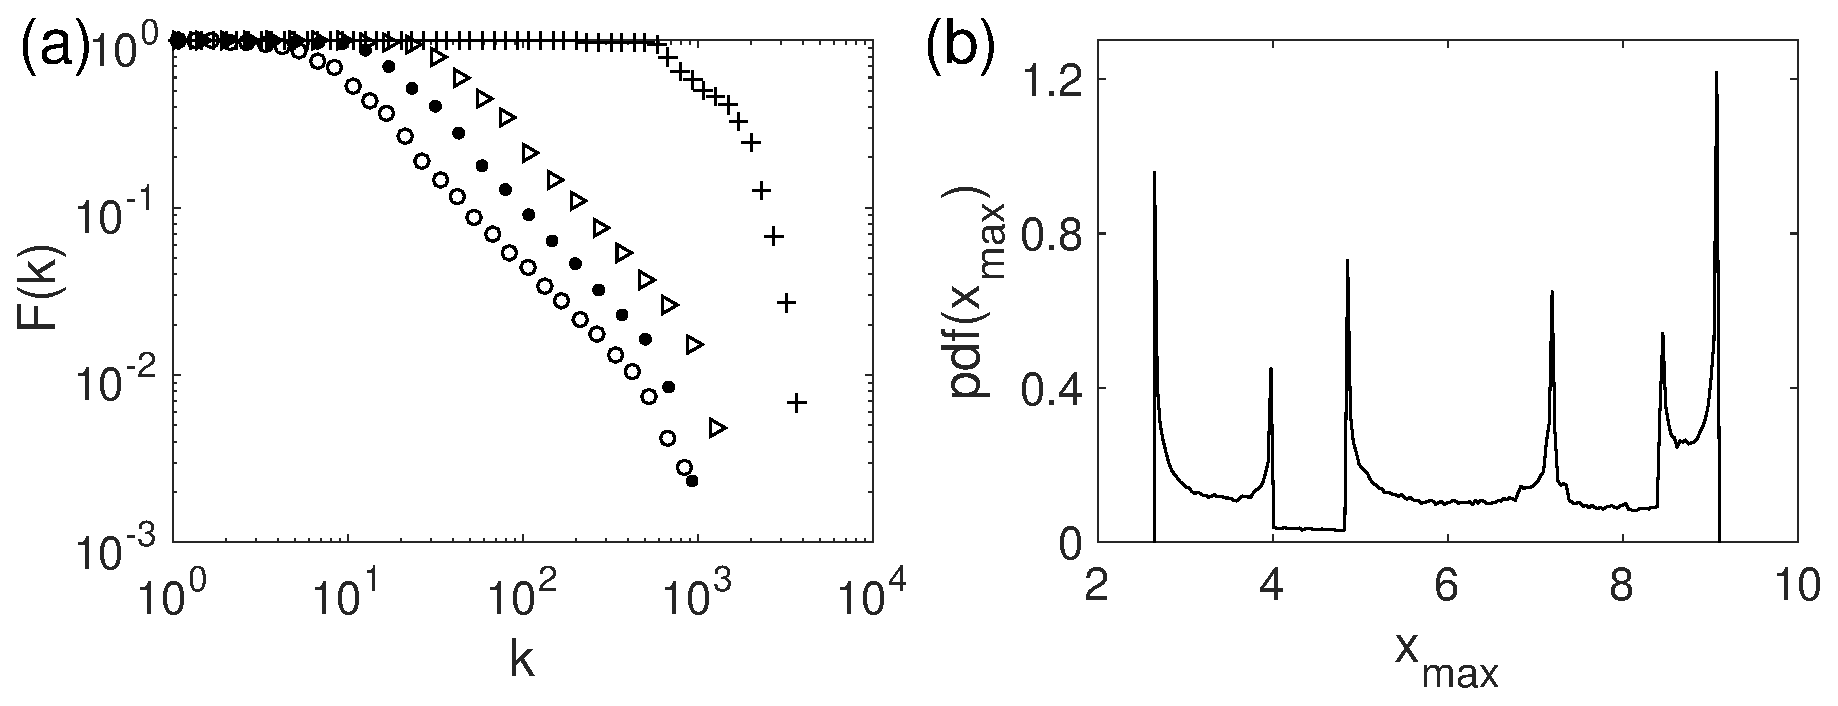
\includegraphics[width=\columnwidth]{Chapter03_RecurrenceNt/retmap_histP.eps}
	\caption{(a) Complementary cumulative distribution function $F(k)=\sum_{k'=k}^{\infty} p(k')$ for RNs obtained from the $x$-component of the first return map of the R\"ossler system (with $a=b=0.2$, $c=5.7$) through the $y=0$ plane, using edge densities $\hat{\rho}_1 =0.02\%$ ($\circ$), $\hat{\rho}_2 =0.03\%$ ($\bullet$), $\hat{\rho}_3 =0.05\%$ ($\triangleright$), and $\hat{\rho}_4 =3\%$ (+). All curves have been obtained as mean values taken from $5$ independent realizations of the system with length $N=2\times 10^5$ and using the Euclidean norm. For $\hat{\rho}_1$ to $\hat{\rho}_3$, we find power-law behavior with a characteristic exponent of $\gamma=2.16\pm 0.03$, whereas no clear scaling region is found in the denser RN with edge density $\hat{\rho}_4$. (b) PDF of the $x$ values, where power-law shaped singularities are observed. Redrawn after \cite{Zou2012}.}
\label{fig:roessler_scaling}
\end{figure}

		Notably, it is not trivial to provide an exhaustive characterization of the conditions under which scale-free distributions can emerge for higher-dimensional systems. As a consequence, generally applicable necessary and sufficient conditions for the presence of power-laws in the degree distributions of RNs have not been established so far. Based on the degree distribution$P(k)$, some higher order statistics have been proposed in \cite{Jocob2016} quantifying the heterogeneity properties of the connectivity. 

		We note that in general complex systems, the emergence of power-laws is often associated with a hierarchical organization related to certain fractal properties. In contrast, for RNs it has been shown that the presence of power-laws is not directly related to some (global) fractal structure of the system, but rather the local shape of its invariant density. Consequently, although there are examples of dynamical systems where the scaling exponent of the degree distribution coincides well with the associated fractal dimension, there is no such relationship in general. It will be subject of future studies under which conditions regarding the structural organization of the attractor, fractal structure and power-law singularities are sufficiently closely related so that the RN's degree distribution allows quantifying the system's fractal properties.
        
       		 \subsubsection{Small-world effect}
		A first generic property shared by many real-world networks is the so-called small-world effect, first described as the outcome of studies on social interrelationships, predominantly Milgram's famous chain-letter experiment in the 1960s \cite{Milgram1967}. In the spirit of the latter studies, the term ``small-world effect'' originally denoted the fact that average shortest path lengths in social networks, but also other real-world networks, are much shorter than we would expect from random connectivity configurations. Given the importance of redundancy in such networks, Watts and Strogatz \cite{Watts1998} suggested including the presence of a high clustering coefficient (i.e., higher than in random graphs) as a second criterion for identifying the small-world effect in real-world networks.

		From the latter considerations, it is clear that RNs cannot obey small-world effects: although they may exhibit a high degree of transitivity (typically depending on the specific system under study), for any \emph{fixed} value of $\varepsilon$ they average path lengths can only take specific values, which become independent of the network size $N$ in case of sufficiently large samples. On the one hand, for any chosen pair of vertices $i$ and $j$ at positions $x_i$ and $x_j$, the shortest path length is bounded from below as $\hat{l}_{ij}\geq \lceil\|x_i-x_j\|/\varepsilon\rceil$ (respectively, the geodesic distance on the attractor $S$ divided by the recurrence threshold $\varepsilon$). Specifically, each shortest path length will converge to a finite value for $N\to\infty$. On the other hand, due to the finite diameter of chaotic attractors, the average path length $\hat{\mathcal{L}}(\varepsilon)$ cannot exceed a maximum value of $\lceil\max_{i,j}\{\|x_i-x_j\|\}/\varepsilon\rceil$ independent of $N$. Hence, the average path length is bounded from above by a value independent of $N$, which is distinct from the common behavior of small-world networks ($\hat{\mathcal{L}}\sim \log N$) \cite{Watts1998}. Moreover, as another immediate consequence of the latter considerations, we observe that $\hat{\mathcal{L}}\sim\varepsilon^{-1}$~\cite{Donner2010a}. This implies that by tuning $\varepsilon$, it is possible to achieve any desired average shortest path length $\hat{\mathcal{L}}$; this fact notably reduces the explanatory power of this global network characteristic.

\todo[inline]{add results from Jacob et al. here; check structure of this section...}


		\subsubsection{Assortative vs. disassortative mixing}
		Unlike small-world effects and scale-free degree distributions, there are hardly any available results regarding the mixing properties of RNs. In general, RNs obey a tendency towards showing assortative mixing (i.e., vertices tend to link to other vertices with similar degree), which is reasonable in situations where the invariant density $p(x)$ is continuous or even differentiable, which is supported by recent numerical results \cite{Donges2011,Donner2010a}. 

		\subsubsection{Path-based characteristics}
		One main field of application of RQA as well as other quantitative approaches to characterizing the distribution of recurrences in phase space (e.g., recurrence time statistics) is identifying and quantifying different degrees of dynamical complexity among realizations of the same system under different conditions (e.g., different values of the control parameter(s)), or even within a single time series given the system is non-stationary. While the line-based characteristics of RQA are founded on heuristic considerations (e.g., the higher the predictability of the observed dynamics, the longer the diagonal line structures off the main diagonal should be), we have argued in Section~\ref{sec:analyticRNtheory} that RNs have an analytical foundation in RGGs. Notably, the corresponding characteristics are based on the same binary structure (the recurrence matrix) as the RQA measures and. Hence, both concepts allow deriving a similar kind of information, with the important difference being that RQA quantifies dynamical properties whereas RNs encode topological/geometric characteristics. However, since both aspects are ultimately linked in the case of chaotic attractors, this general observation suggests that RN analysis is in principle suitable for characterizing dynamical complexity in the same way as other established concepts. Therefore, one natural question arises: How do RN measures perform in this task, and which of the multiple possible network measures are particularly suited for this purpose?

		The latter questions have been the main motivation behind much of the early work on RNs focussing on numerical studies of various paradigmatic model systems for low-dimensional chaos~\cite{Donner2010Nolta,Donner2011,Donner2010b,Donner2010a,Marwan2009,Zou2010,Zou2012c}. The latter studies suggest that for characterizing dynamical complexity, global network characteristics are conceptually easier to use and could provide potentially more stable and distinctive results than certain statistics over local network properties such as the distributions of vertex degrees~\cite{Zou2012b} or local clustering coefficients~\cite{Zou2012c}. Among the set of possible global RN measures, two properties have been found particularly useful: network transitivity $\hat{\mathcal{T}}$ and average path length $\hat{\mathcal{L}}$.

		Regarding the average path length, the discriminatory skills regarding different degrees of dynamical complexity can be understood by the fact that for time-continuous systems, chaotic systems can display different degrees of spatial filling of the ``populated'' area in phase space, i.e., a high (fractal) dimension of a chaotic attractor close to the (integer) dimension of the corresponding phase space gives rise to a more homogeneous filling than lower ones, which has a natural geometric consequence for the possible path lengths between pairs of sampled state vectors on the attractor. However, it needs to be noted that quantifying dynamical complexity by means of $\hat{\mathcal{L}}$ suffers from two important drawbacks: 

		On the one hand, the measure is not normalized and depends crucially on the choice of $\varepsilon$. Hence, working in different methodological settings (e.g., using fixed recurrence thresholds $\varepsilon$ vs. fixed recurrence rates $RR=\hat{\rho}$) can provide potentially ambiguous results, since numerical values of $\hat{\mathcal{L}}$ cannot necessarily be directly compared with each other. 

		On the other hand, even the qualitative behavior of $\hat{\mathcal{L}}$ in dependence on the system's dynamical complexity depends on whether the system is a discrete map or time-continuous. In the latter case, a periodic orbit would result in a higher average path length than a chaotic one, since a chaotic attractor is a ``spatially extended'' object in phase space on which there are ``shortcuts'' between any two state vectors connecting points corresponding to different parts of the trajectory~\cite{Donner2010a}. In turn, for discrete maps, a periodic orbit contains only a finite set of $p$ mutually different state vectors, so that for sufficiently low $\varepsilon$ and large $N$, the RN is decomposed into $p$ disjoint, fully connected components. In such a situation with not just single isolated vertices, but a completely decomposed network, a reasonable redefinition of $\hat{\mathcal{L}}$ would be summing up only over pairs of mutually reachable vertices in Eq.~(\ref{eq:aplRN}). Consequently, we approach the minimum possible value of $\hat{\mathcal{L}}=1$~\cite{Marwan2009}, whereas chaotic orbits typically lead to larger $\hat{\mathcal{L}}$.

		According to the above observations, there is no fully developed theoretical understanding and description of the influence of attractor dimensionality on the resulting average path length beyond the general considerations presented in Section~\ref{sec:analyticRNtheory}. Corresponding further investigations might be an interesting subject for future studies.

       		 \subsubsection{Dimension characteristics by clustering and transitivity} \label{sec:transitivity}
		As mentioned in Section~\ref{sec:scaling}, the scaling exponent of a possible power-law degree distribution has no direct relationship to the fractal dimension of the system. In turn, such a relationship naturally exists when studying the corresponding integrated measure (i.e., the edge density $\hat{\rho}(\varepsilon)$) in terms of its scaling properties as the recurrence threshold is systematically varied. The latter approach has been extensively discussed in the literature in connection with the estimation of dynamical invariants from RPs~\cite{Faure1998,thiel2004a} and gives rise to estimates of the correlation dimension $D_2$. Notably, one of the classical approaches to estimating $D_2$ from time series data, the Grassberger-Procaccia algorithm~\cite{Grassberger1983PLA,Grassberger1983PRL}, makes use of the correlation sum, which can be easily formulated in terms of the recurrence rate or RN edge density.

		The relatively high computational complexity of the latter approaches to estimating the correlation dimension from a RP stems from the fact that a sequence of RPs for different values of $\varepsilon$ needs to be studied for obtaining a proper scaling relationship. In turn, as shown by us in previous studies~\cite{Donner2011b}, network transitivity provides an alternative approach to defining and estimating a different notion of fractal dimension. For this purpose, note that for a classical RGG embedded in some integer-dimensional metric space, the expected network transitivity (which is numerically estimated as the ensemble mean over sufficiently many realizations of the stochastic generation of the RGG) is an analytical function of the dimension $m$, which decays (exactly when using the maximum norm, otherwise approximately) exponentially with $m$~\cite{Dall2002}. This analytical relationship can be generalized to attractor manifolds with non-integer fractal dimensions, which can in turn be estimated from the RN transitivity by inverting this function.

		\paragraph{Transitivity dimensions}
		For the general case, the latter idea leads to a pair of quantities referred to as upper and lower transitivity dimensions \cite{Donner2011b},
\begin{eqnarray}
D_{\mathcal{T}}^u &=& \limsup_{\varepsilon} \frac{\log(\mathcal{T}(\varepsilon))}{\log(3/4)}, \label{eq:dtu} \\
D_{\mathcal{T}}^l &=& \liminf_{\varepsilon} \frac{\log(\mathcal{T}(\varepsilon))}{\log(3/4)}, \label{eq:dtl}
\end{eqnarray}
\noindent
where the two definitions originate from the fact that certain systems (in particular, chaotic maps whose attractors form Cantor sets in at least one direction in phase space~\cite{Donner2011b}) can exhibit an oscillatory behavior between some upper and lower accumulation point of $\mathcal{T}(\varepsilon)$ as the recurrence threshold $\varepsilon$ is varied. For systems without such fragmented structure, upper and lower transitivity dimension seem to coincide, which allows estimating them from the sample RN transitivity with reasonable accuracy using only a single network instance with one suitably chosen value of $\varepsilon$. A detailed analytical investigation of the qualitatively different behavior of the RN transitivity for chaotic attractors with continuous and fragmented invariant densities in dependence on $\varepsilon$ will be subject of future work. Note that in the above definition, we do not explicitly consider a scaling behavior for $\varepsilon\to 0$, since the definition does not explicitly contain $\varepsilon$ (as it is the case for other classical notions of fractal dimensions), but makes use of normalized characteristics with a probabilistic interpretation (cf. Section~\ref{sec:analyticRNtheory}). In this spirit, the fraction on the right-hand side of the former equations is a well-defined object for each value of $\varepsilon$ (i.e., the specific scale under which the system is viewed) individually.

% Figure~\ref{fig:roessler_transitivity}A shows the behavior of the scale-dependent transitivity dimension estimate $\hat{D}_{\mathcal{T}}(\varepsilon)=\log(\hat{\mathcal{T}}(\varepsilon))/\log(3/4)$ for the R\"ossler system (Eq.~\ref{eq:roessler}) for three different RN sizes. 
		More numerical results have been presented in \cite{Donges2012}. We clearly recognize that $\hat{D}_{\mathcal{T}}(\varepsilon)$ assumes approximately stable (i.e., $N$- and $\varepsilon$-independent) values if the recurrence threshold is chosen sufficiently large. In general, there exist two limits that need to be taken into account: For too large recurrence rates, the RN characteristics lose their discriminatory skills, since too many edges are present masking subtle small-scale properties of the attractor \cite{Donges2012,Donner2010b}. In turn, if $\varepsilon$ is too low (e.g., if $\hat{\rho}$ is below the RN's percolation threshold) \cite{Donges2012}, the network decomposes into mutually disjoint components, and the resulting network characteristics can become ambiguous. %In the considered example of the R\"ossler system, this decomposition is mainly caused by the rare excursions of some cycles towards larger $z$ values, which give rise to a poorly populated region (low $p(x)$) of the attractor. In order to properly cover this part of the attractor for a given $\varepsilon$, many samples (i.e., a large network size $N$) are necessary. Otherwise, the edge density $\hat{\rho}$ starts saturating as $\varepsilon$ gets smaller (at least in the regime where most vertices close to the $z=0$ plane are still connected, cf. Fig.~\ref{fig:roessler_transitivity}B), and the transitivity dimension estimates strongly deviate from their expected values.

		Notably, the analytical relationship (Eqs.~\ref{eq:dtu},\ref{eq:dtl}) between the effective (geometric) dimension of chaotic attractors and RN transitivity provides the theoretical justification and foundation for applying $\hat{\mathcal{T}}$ as a characteristic discriminating between high and low dynamical complexity of chaotic attractors. Unlike for $\hat{\mathcal{L}}$, the transitivity shows qualitatively the same behavior for discrete and time-continuous systems and is normalized, so that its values can be directly used as a quantitative measure of dynamical complexity associated with the effective geometric dimensionality and, hence, structural complexity of the attractor in phase space.


\todo[inline]{relationship with classical R\'enyi dimensions (discussions with Grassberger)}
        
\todo[inline]{add brief information on behavior of other network characteristics?}


		\paragraph{Clustering dimension}\label{sec:transitivity_local}
		With the same rationale as for the global network transitivity, we can make use of the local clustering properties of RNs for defining local measures of attractor dimensionality, referred to as upper and lower clustering dimensions~\cite{Donner2011b}:
\begin{eqnarray}
D_{\mathcal{C}}^u(x) &=& \limsup_{\varepsilon} \frac{\log(\mathcal{C}(x;\varepsilon))}{\log(3/4)}, \\
D_{\mathcal{C}}^l(x) &=& \liminf_{\varepsilon} \frac{\log(\mathcal{C}(x;\varepsilon))}{\log(3/4)}.
\end{eqnarray}
\noindent
Following the same argument as for the (global) transitivity dimensions, we do not need to consider the limit $\varepsilon\to 0$ here.

		With similar considerations regarding the possible existence of two distinct accumulation points of $\mathcal{C}(x)$ as $\varepsilon$ varies, we may utilize this framework for characterizing the point-wise dimension of chaotic attractors in a unique way without making explicit use of scaling characteristics as in the common point-wise dimensions~\cite{Donner2011b}. However, we need to keep in mind that the considered concept of (geometric) dimensionality is largely affected by the profile of the invariant density, e.g., the existence of sharp attractor boundaries or supertrack functions~\cite{Donner2010Nolta,Donner2011b,Donner2010a}. For example, if the attractor has distinct tips (e.g., in the case of the H\'enon system~\cite{Donner2011b,Donner2010a}), the geometric dimension at these points is effectively reduced to zero, which is reflected by $\hat{\mathcal{C}}_v=1$ for vertices $v$ sufficiently close to the tips. A similar behavior can be observed for the logistic map at the attractor boundaries and the supertrack functions~\cite{Donner2010Nolta,Donner2011b,Donner2010a}.

		The latter observations point to a prospective application of the local clustering properties of RNs. In case of chaotic attractors of time-continuous dynamical systems, it is known that an infinite number of unstable periodic orbits (UPOs) provide the skeleton of the chaotic dynamics and are densely embedded in the attractor. The localization of such UPOs is, however, known to be a challenging task. Since UPOs are relatively weakly repulsive (from a practical perspective, those UPOs with low periods are typically least unstable), a trajectory getting close to the vicinity of an UPO will stay close to this orbit for some finite amount of time~\cite{Lathrop1989}. As a result, the dynamics close to UPOs is quasi one-dimensional, and state vectors sampled from the trajectories approximate some lower-dimensional (in the limiting case one-dimensional) subset of the attractor manifold. In such case, the above theoretical considerations suggest that the local clustering coefficient $\hat{\mathcal{C}}_v$ of vertices $v$ close to low-periodic UPOs should be higher than the values typical for other parts of the chaotic attractor. This conceptual idea is supported by numerical results from our previous work~\cite{Donner2010b,Donner2010a} (cf.\, also the band structures with increased $\hat{\mathcal{C}}_v$ in Fig.~\ref{fig:local}(b)), but has not yet been systematically applied to the problem of UPO localization. Notably, the detection limit of UPOs should be ultimately determined by the recurrence threshold $\varepsilon$ in conjunction with the RN size $N$. Specifically, for every finite $\varepsilon>0$, there are infinitely many UPOs intersecting with the $\varepsilon$-neighborhood of some point $x_v$ in phase space, whereas we will (for a finite sample of state vectors) only resolve the signatures of the least unstable orbits.


	\subsection{Practical considerations} \label{subsec:practicalRN}
		\subsubsection{Dependence on embedding parameters}
		We focus on two important algorithmic parameters of the RN approach, embedding dimension and delay. The impact of other parameters such as recurrence threshold $\varepsilon$, sampling rate, or even the selection of variables in multi-dimensional systems has been extensively discussed elsewhere~\cite{Donner2010b,Strozzi2009} for deterministic systems, but not yet for stochastic ones. For the sake of brevity, we present only a brief corresponding discussion here. Specifically, since we consider discrete-time univariate stochastic processes, only $\varepsilon$ is relevant, but can be treated mostly alongside the theoretical considerations presented in~\cite{Donges2012}.
		
		Given a scalar time series $\{x_i\}$ ($i=1,\dots,N$), in order to apply RN analysis we first have to convert the data into state vectors in some appropriately reconstructed phase space. A common method from dynamical systems theory to define such a phase space is time-delay embedding~\cite{Takens1981}. In fact, the concept of a phase space representation rather than a ``simple'' time or frequency domain approach is the hallmark of many methods of nonlinear time series analysis, requiring embedding as the first step. Here, we define $\mathbf{x}_i = (x_i, x_{i-\tau}, \cdots, x_{i-(m-1)\tau})$ to obtain an $m$-dimensional time-delay embedding of $x_i$ with embedding delay $\tau$ for obtaining state vectors in phase space~\cite{Takens1981}. It has been proven that for deterministic dynamical systems, the thus reconstructed phase space is topologically equivalent to the original space if $m > 2 D_F$, where $D_F$ is the fractal dimension of the support of the invariant measure generated by the dynamics in the true (but often at most partially observed) state space. Note that $D_F$ can be much smaller than the dimension of the underlying original (physical) phase space spanned by all relevant system variables.

		From a practical perspective, when analyzing a scalar time series of whatever origin, neither embedding dimension $m$ nor delay $\tau$ are known a priori. The false nearest-neighbors (FNN) method~\cite{Kennel1992} was introduced to derive a reasonable guess of how to choose $m$ based on studying whether or not proximity relations between state vectors are lost when the embedding dimension is successively increased. If a reasonable embedding dimension is found, all dynamically relevant coordinates of the system are appropriately represented, so that all proximity relationships are correct and not due to lower-dimensional projection effects. In a similar spirit, the first root of the auto-correlation function (ACF) of a time series often yields a good estimate for $\tau$. A more refined method is to use time-delayed mutual information~\cite{Fraser1986}.

		The aforementioned approaches to determining $m$ and $\tau$ commonly work well for data from deterministic dynamical systems. Embeddings are not applicable for non-stationary processes though they are more ubiquitous in real time series analysis, for instance, fractional Brownian motions (fBm) and related processes arising from an integration of stationary processes (e.g., fractional L\'evy motion, (F)ARIMA models, etc.). More specifically, we have to keep in mind some severe conceptual problems may appear when applying them to non-stationary processes: First, finite estimates of $D_F$ are spurious due to the finite amount of data used. The latter result is reasonable since an infinite amount of data (i.e., the innovations at each time step) are necessary to fully describe the evolution of a stochastic process. Thus, from a conceptual perspective, the embedding dimension should be chosen infinitely large. In turn, finite $m$ will necessarily cause spurious results since the full complexity of the system's (discrete) trajectory is not captured.
		
		On the other hand, the embedding delay $\tau$ is not considered in the mathematical embedding theorems for deterministic dynamical systems. Embeddings with the same embedding dimension $m$ but different $\tau$ are topologically equivalent in the mathematical sense~\cite{kantz1997}, but in reality a good choice of $\tau$ facilitates further analysis. If $\tau$ is small compared to the relevant internal time-scales of the system, successive elements of the delay vectors are strongly correlated. This leads to the practical requirement that the embedding delay should cover a much longer time interval than the largest characteristic time-scale that is relevant for the dynamics of the system. However, in fBm arbitrarily long time-scales are relevant due to the self-similar nature of the process \cite{Zou2015}. This makes finding a feasible value of $\tau$ a challenging (and, regarding formal optimality criteria, even theoretically impossible) task.
		
		We emphasize that in the case of non-stationary fBm, the fundamental concepts of phase space reconstruction and low-dimensional dynamics do not apply (not even approximately) anymore. Therefore, any attempt to applying RN analysis to fBm directly necessarily yields results that hold only for the particular embedding parameters chosen and the specific length of the given time series~\cite{Liu2014}.  In \cite{Zou2015}, we have demonstrated that RN analysis can indeed provide meaningful results for stationary stochastic processes, given a proper selection of its intrinsic methodological parameters, whereas it is prone to fail to uniquely retrieve RN properties for non-stationary stochastic processes like fBm. In cases of non-stationarity, a proper transformation is required to remove the particular type of non-stationarity from the data. This can be achieved by additive detrending, phase adjustment (de-seasonalization), difference filtering (incrementation) or other techniques, with the one mentioned last being the proper tool for the particular case of fBm transforming the original process into stationary fractional Gaussian noise.
		
		\subsubsection{Choice of recurrence rate or threshold} \label{subsub:epsilon}
        		The crucial algorithmic parameter of recurrence-based time series analysis is  $\varepsilon$, which has been discussed extensively  in the literature \cite{marwan2007,Donner2010b}. The more empirical choice of $\varepsilon$ often depends on time series embedded in phase space. Too small $\varepsilon$ causes very sparsely connected RN with many isolated components; too large $\varepsilon$ results in an almost completely connected network. Several invariants of a dynamical system  e.g., the second-order R\'enyi entropy $K_2$  can be estimated by taking its recurrence properties for $\varepsilon \to 0$ \cite{Grassberger1983PLA,Grassberger1983PRL}, which suggests that for a feasible analysis of recurrence networks, a low $\varepsilon$ is preferable as well. This is supported by the analogy to complex networks based on spatially extended systems, where attention is usually restricted to the strongest links between individual vertices  i.e., observations from different spatial coordinates for retrieving meaningful information about relevant aspects of the systems' dynamics. In contrast, a high edge density, does not yield feasible information about the actually relevant structures, because these are hidden in a large set of mainly less important edges \cite{Donner2010b}.

		As a consequence, only those states should be connected in a recurrence network that are closely neighbored in phase space, leading to rather sparse networks. Following a corresponding rule of thumb confirmed for recurrence quantification analysis \cite{schinkel2008}, we suggest choosing $\varepsilon$ as corresponding to an edge density $\rho \lesssim 0.05$ \cite{Marwan2009,Donner2010a}, which yields neighborhoods covering appropriately small regions of phase space. Note that since many topological features of recurrence networks are closely related to the local phase space properties of the underlying attractor~\cite{Donner2010a}, the corresponding information is best preserved for such low $\varepsilon$ unless the presence of noise requires higher $\varepsilon$ \cite{schinkel2008}. 

		The heuristic criterion proposed by Gao {\textit{et al.}} \cite{Gao2009}, which selects $\varepsilon$ as the (supposedly unique) turning point of the plot of $\rho$ vs. $\varepsilon$, is \textit{not} generally applicable as we have discussed in \cite{Donner2010b}. In particular, this heuristic criterion can \textit{not} attribute certain network features to specific \textit{small-scale} attractor properties in phase space \cite{Donner2010b}. Moreover, besides our general considerations supporting low $\varepsilon$, application of the turning point criterion leads to serious pitfalls. One has to emphasize that various typical examples for both discrete and continuous dynamical systems are characterized by \textit{several} turning points. Depending on the particular types of signals from real measurements from civil engineering structures, surrogate-assisted method for choosing optimal threshold by searching for a turning point of proper defined quality loss function might be a good solution \cite{Yang2015a}. 
        
        		One of the problems preventing a uniform choice of $\varepsilon$ between different time series is that the size of the attractor after embedding is arbitrary. To overcome this, Jacob \cite{Jacob2016b} proposed first to transform the time series into a uniform deviate so that the size of the attractor gets rescaled into the unit interval $[0, 1]$. Then, their choice of $\varepsilon$ is based on empirical results from numerical computations such that the following two criteria are fulfilled \cite{Jacob2016b}: a) the resulting RN has to remain mostly as ``one single cluster" and b) the measures derived from the RN should uniquely represent the underlying attractor. Note that the first condition fixes the lower bound for $\varepsilon$ which ensures the network becomes fully connected. The second one fixes the upper bound. Furthermore, they show that the above two conditions together provide an identical optimum $\varepsilon$ range for time series from all chaotic attractors. It should be noted that the above choice of the critical range of $\varepsilon$ is, in fact, analogous to the selection of a scaling region in the conventional nonlinear time-series analysis for computing dynamical invariants like correlation dimension $D_2$ \cite{Grassberger1983PLA}.
		
		The above strategies in choosing $\varepsilon$ help us to overcome the problem of sliding-window-based analyses of systems with varying amplitude fluctuations (as coming from different dynamical regimes or non-stationarities), for instance, those based on normalizing time series or fixing recurrence density. However, in real-world applications, time series are not usually smooth all the time. When considering the time series by a RN representation, extreme points (very high jumps or falls in the fluctuation of time series) in the time series could break the connected components in the network since the distance between an extreme point and other points would be larger than the threshold value \cite{Eroglu2014}. These unconnected components would cause problems for some complex network measures, since some of them need a connected network to be computed for the entire network. For example, even if we have just one node that is not connected to the network, the average path length will always be infinite for the entire network. The normalization method would then result in non-optimal recurrence thresholds biasing the recurrence analysis. An even more important motivation for avoiding isolated components in the RN is that the RN provides a large amount of information about the dynamics of the underlying system, although it contains only binary information. To find a sufficiently small threshold $\varepsilon$ that fulfills the desired condition of connected neighborhoods, Eroglu {\textit{et al.}} proposed to use the connectivity properties of the network. In particular, they choose the value for $\varepsilon$ that is the smallest one for the RN to be connected. The connectivity of a RN is measured by the second-smallest eigenvalue $\lambda_2$ of the Laplacian matrix associated to the recurrence matrix \cite{Eroglu2014}. Note that this criterion in choosing an adaptive $\varepsilon$ shares the same idea as used \cite{Jacob2016b,Lin2016}. Note that in the case that phase space is consisted by several disjoint partitions, the method guaranteeing the connectivity might not be feasible, for instance, phase space is not continuous when the control parameter is before the band merging of the Logistic map. Another counter examples has been presented in the standard map where there are several components in phase space \cite{Donner2010b,Zou2016d}). 
		 
		 As mentioned before, small variations of $\varepsilon$ may lead to very different modular structure in the associated recurrence network, which prompts a big challenge for identifying metastable states in real-world time series. Note that modular regions of RNs may correspond to trajectory bundle, which are associated to the existence of metastable states. This way, selecting an inadequate recurrence threshold can hide important geometric information of the state space of a system. In \cite{Vega2016}, the authors suggested that an adequate recurrence threshold should lie in a range of values producing recurrence networks with similar modular structures. This means that there is a range of recurrence thresholds for which the associated recurrence networks describe reconstructed state spaces with equivalent topology. However, this region of values depends on the distribution of the particular time series data, which might not be uniform. To this end, they define a filtration procedure to self-adaptively set an adequate $\varepsilon$ from RNs that are associated to a set of recurrence thresholds. The adequate $\varepsilon$ belongs to the subset of values in the filtration for which the modular structures of their associated RNs are the least dissimilar. Furthermore, in searching for metastable states \cite{Vega2016}, the authors suggested to compute modular similarity measures like the Adjusted Rank Index, which then further help to compute the final adequate recurrence threshold $\varepsilon$. 	
		 
		\subsubsection{Stability and robustness against noise}
        		The results of the previous subsections show that RN approaches are able to clearly distinguish between periodic and chaotic dynamics under noise free condition. In experimental time series, one is always confronted with measurement errors. Hence, it is necessary to analyze the influence of noise on the reconstructed RNs. In the framework of recurrence plot, a larger $\varepsilon$ has been suggested to overcome the noise effect \cite{thiel2002}, for instance, a threshold $\epsilon$ that is at least 5 times the standard deviation of the observational Gaussian noise $\sigma$ can yield reliable statistics. This criterion is based on the analytical computation of the probability of a recurrence point in the RP to be correctly recognized in the presence of observational noise. We suggest to use this criterion if weak observational noise is present as it has been found that the choice $\epsilon \sim 5\sigma$ is optimal for a wide class of processes \cite{thiel2002}. 		
	
		Furthermore, in \cite{Subramaniyam2014} the authors show that the influence of noise on the network measure $\mathcal{C}$ can be minimized by an appropriate choice of $\rho(\varepsilon)$ (e.g., by setting $\rho(\varepsilon) > 0.02$), while the influence on $\mathcal{L}$ is independent of $\rho(\varepsilon)$. However, for noise levels greater than 40\% in case of $\mathcal{C}$ and 20\% in case of $\mathcal{L}$, the recurrence network measures fail in distinguishing between noisy periodic dynamics and noisy chaotic dynamics. 
		
		It is also possible to test the efficiency of RN measures as discriminating statistics by means of hypothesis testing using surrogate technique \cite{Jacob2018}. For instance, network measures of RNs are effective if the data involves both white noise and colored noise, which have been further illustrated by experimental time series that has been simulated by a black hole light curves model.          
        
        		\subsubsection{Behavior for larger $\varepsilon$}
        new papers by Jacob et al., cross-over to small-world (spatial network like) behavior

	
	\subsection{Multiplex recurrence networks}
	So far, RN approaches has been discussed in the framework of a single system. In the next two subsections, we focus on several different generalizations to multivariate analysis, for instance, multiplex recurrence networks (MRN) and two different versions of multilayer recurrence networks: inter-system recurrence networks (ISRN) and joint recurrence networks (JRN) which are based on cross recurrence plots and joint recurrence plots respectively. 

		Let us start with the construction of multiplex recurrence networks, as schematically illustrated in Fig. \ref{fig:multiRN}. If in a multilayer network of $M$ layers, each layer has the same set of vertices and the connections between layers are only between a node and its counterpart in the other layers, then we call such networks ``multiplex". In \cite{Eroglu2018}, Eroglu {\textit{et al}} proposed to construct multiplex recurrence networks, which shares much similarities in constructing multiplex visibility graphs \cite{Lacasa2015b}. Consider an $M$-dimensional multivariate time series $\{{\bf{x}}(t) \}_{t=1}^{n}$, with ${\bf{x}}(t) = (x^{[1]}(t), x^{[2]}(t), \dots, x^{[M]}(t)) \in \mathbb{R}^M$ for any value of $t$. Then, the RN of the $\alpha$th component of ${\bf{x}}(t)$ is created and located into the associated layer $\alpha$ of the multiplex network. For the $M$-dimensional multivariate time series, we can create $M$ different RNs which have the same number of nodes and each node is labeled by its associated time. These networks will form the different layers of a multilayer network. The layers are connected each other with the same time labeled nodes. Furthermore this procedure requires that the time sampling is the same for all of the used time series.  Networks, transformed from multivariate time series, are compatible with the definition of multiplex networks, because each node is uniquely assigned to a certain time point of the multivariate time series, i.e., we find the equally time-labeled nodes in all layers. 
		
		{\color{red} can I get the source figure from Deniz? Figure 1 to explain the construction steps, highly acknowledged.} 
		\begin{figure}
			\centering
			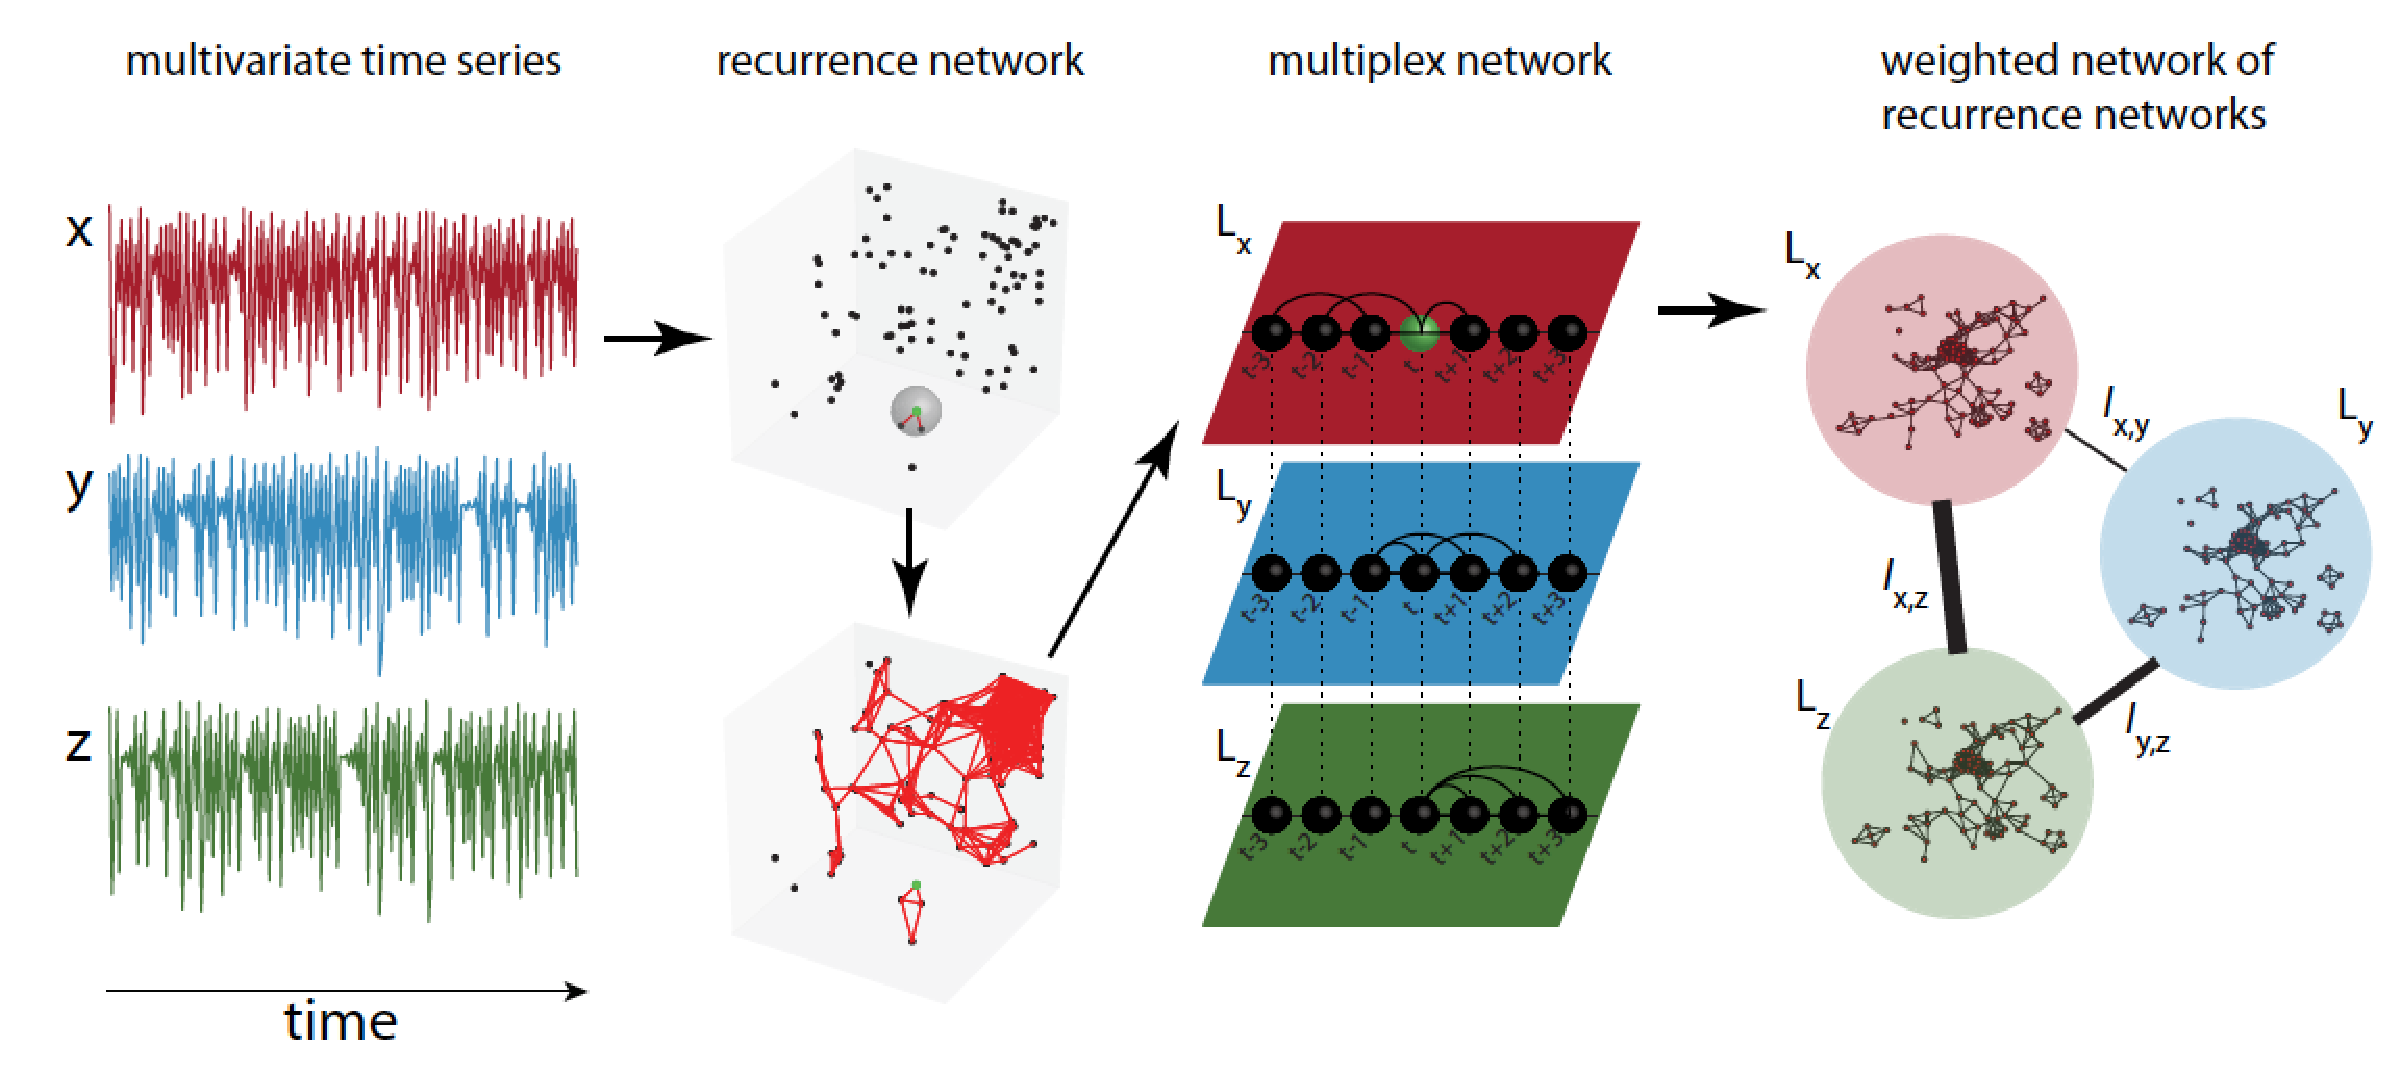
\includegraphics[width=\columnwidth]{Chapter03_RecurrenceNt/multiPrn.eps}
		\caption{\small{Construction of multiplex recurrence networks for multivariate time series. Courtesy of \cite{Eroglu2018}. } \label{fig:multiRN}}
		\end{figure}
		
		More specifically, we denote the adjacency matrix of the $\alpha$th layer as $A^{[\alpha]} = a_{ij}^{[\alpha]}$ and $a_{ij}^{\alpha} = 1$ if nodes $i$ and $j$ are connected in layer $\alpha$, $a_{ij}= 0$ otherwise. Then the entire multiplex network $\mathcal{A}$ is represented by the vector of adjacency matrices of its layers $\mathcal{A} = \{A^{[1]}, A^{[2]}, \dots, A^{[M]}\}$, which read 
		\begin{equation}
\mathcal{A} = \left[ \begin{array}{cccc}
\mathbf{A}^{[1]} & \mathbf{I}_{[N]} & \ldots             & \mathbf{I}_{N}\\
\mathbf{I}_{[N]} & \mathbf{A}^{[2]} & \ddots             & \vdots   \\
\vdots                & \ddots                & \ddots            & \mathbf{I}_{N} \\
\mathbf{I}_{[N]} & \ldots                 & \mathbf{I}_{N} & \mathbf{A}^{[m]}\\
\end{array} \right]_{Nm \times Nm}, 
		\end{equation}
where $\mathbf{I}_{N}$ is the identity matrix of size $N$. 

		Two different measures have been proposed to quantify the similarity between layer $\alpha$ and $\beta$ of the giant multiplex network \cite{Eroglu2018,Lacasa2015b}. The first is to compute the interlayer mutual information $I_{\alpha, \beta}$: 
		\begin{equation} \label{eq:RNmultiplex}
		I_{\alpha, \beta} = \sum_{k^{[\alpha]}} \sum_{k^{[\beta]}} P(k^{[\alpha]}, k^{[\beta]}) \log \frac{P(k^{[\alpha]}, k^{[\beta]})}{P(k^{[\alpha]}) P(k^{[\beta]}) }, 
		\end{equation}
where $P(k^{[\alpha]}, k^{[\beta]}) $ is the joint probability of the existence of nodes which has $k^{[\alpha]}$ degree at layer $\alpha$ and $k^{[\beta]}$ at layer $\beta$, $P(k^{[\alpha]})$ and $P(k^{[\beta]}) $ are the degree distributions of RNs at layer $\alpha$ and $\beta$ respectively. Since $I_{\alpha, \beta}$ is computed based on the degree sequences, instead of the original time series, the mutual information $I_{\alpha, \beta}$ considers the topological recurrence structures in phase space. 

		Another measure to quantify the coherence of the original multivariate system is the average edge overlap \cite{Eroglu2018,Lacasa2015b}: 
		\begin{equation} \label{eq:RNmultiplexW}
			\omega = \frac{\sum_i\sum_{j>i} \sum_{\alpha}a_{ij}^{[\alpha]}}{m \sum_i\sum_{j>i}(1-\delta_{0, \sum_{\alpha}a_{ij}^{[\alpha]}})}, 
		\end{equation}
		where $\delta_{ij}$ is the Kronecker delta symbol. This measure represents the average number of identical edges over all layers of the multiplex network \cite{Lacasa2015b}. Like the interlayer mutual information Eq. \eqref{eq:RNmultiplex}, $\omega$ estimates the similarity and coherence with averaged existence of overlapped links from nodes $i$ to $j$ between all layers $\alpha$ and $\beta$. 
		
		Note that the interlayer similarity measures (Eqs. \eqref{eq:RNmultiplex}, \eqref{eq:RNmultiplexW}) are computed for each pair layers. The giant adjacency matrix $\mathcal{A}$ of the multiplex network can be projected onto one weighted network representation encompassing the interlayer information only. In other words, we consider each single layer of the multiplex as a node and weighted edges between nodes $\alpha$ and $\beta$ are determined by the quantity $I_{\alpha, \beta}$, which yields that the size of the projection weighted network $M \times M$. 
		
		
	\subsection{Multilayer networks: coupled networks}
    		\subsubsection{General preliminaries}
		When describing multilayer and multiplex networks, we introduced the traditional notations in Sec. \ref{sec:multiplex}. However, in the particular case of networks reconstructed from two or more interacting time series, we prefer to utilize a recently introduced general framework \cite{Donges2011b,Wiedermann2013}. Let us consider an arbitrary undirected and unweighted simple graph $G=(V,E)$ with adjacency matrix $\textbf{A}=\{A_{ij}\}_{i,j=1}^N$. Furthermore, let us assume that there is a given partition of $G$ with the following properties:
\begin{enumerate}
\item The vertex set $V$ is decomposed into $K$ disjunct subsets $V_k \subseteq V$ such that $\bigcup_{k=1}^K V_k = V$ and $V_k \cap V_l = \emptyset$ for all $k \neq l$. The cardinality of $V_k$ will be denoted as $N_k$. 
\item The edge set $E$ consists of mutually disjoint sets $E_{kl} \subseteq E$ with $\bigcup_{k,l=1}^K E_{kl} = E$ and $E_{kl} \cap E_{mn}=\empty$ for all $(k,l) \neq (m,n)$.
\item Let $E_{kl}\subseteq V_k\times V_l$. Specifically, for all $k=1,\dots,K$, $G_k=(V_k,E_{kk})$ is the induced subgraph of the vertex set $V_k$ with respect to the full graph $G$.
\end{enumerate}
Under these conditions, $E_{kk}$ comprises the (internal) edges within $G_k$, whereas $E_{kl}$ contains all (cross-) edges connecting $G_k$ and $G_l$. Specifically, for the ``natural'' partition of an IRN, the $G_k$ correspond to the single-system RNs constructed from the systems $X_k$, whereas the cross-recurrence structure is encoded in $E_{kl}$ for $k \neq l$.

		We are now in a position to study the interconnectivity structure between two subnetworks $G_k, G_l$ on several topological scales drawing on the lineup of local and global graph-theoretical measures generalizing those used for single network characterization (Section~\ref{sec:rn_measures}). In this context, local measures $\hat{f}_v^{kl}$ characterize a property of vertex $v \in V_k$ with respect to subnetwork $G_l$, while global measures $\hat{f}_{kl}$ assign a single real number to a pair of subnetworks $G_k, G_l$ to quantify a certain aspect of their mutual interconnectivity structure. Most interconnectivity characteristics discussed below have been originally introduced in \cite{Donges2011b} which see for more detailed discussions.

		\subsubsection{Vertex characteristics}
		The \textit{cross-degree} (or \textit{cross-degree centrality})
\begin{equation}
\hat{k}_v^{kl} = \sum_{i \in V_l} A_{vi}
\label{eq:degree_cross}
\end{equation}
counts the number of neighbors of $v$ within $G_l$, i.e., direct connections between $G_k$ and $G_l$ (Fig.~\ref{fig:interacting_measures}A). Thus, this measure provides information on the relevance of $v$ for the network ``coupling'' between $G_k$ and $G_l$\footnote{In the specific case of an IRN, we interpret this as geometric signatures of the coupling between the underlying dynamical systems $X_k$ and $X_l$~\cite{Feldhoff2011,Feldhoff2012}.}. For the purpose of the present work, it is useful studying a normalized version of this measure, the \textit{cross-degree density}
\begin{equation}
\hat{\rho}_v^{kl} = \frac{1}{N_l} \sum_{i \in V_l} A_{vi} = \frac{1}{N_l} \hat{k}_v^{kl}.
\label{eq:locrho_cross}
\end{equation}
\noindent
For an IRN, $\hat{\rho}_v^{kl}(\varepsilon_{kl})$ equals the (cross-) recurrence rate $RR_{kl}(\varepsilon_{kl})$ (for $k=l$, it gives the corresponding single-system recurrence rate $RR_k(\varepsilon_k)$).

		As for the single network case, important information is governed by the presence of triangles in the network. Given two subnetworks, the \textit{local cross-clustering coefficient}
\begin{equation}
\hat{\mathcal{C}}_v^{kl} = \frac{1}{\hat{k}_v^{kl}(\hat{k}_v^{kl} - 1)} \sum_{i,j \in V_l} A_{vi} A_{ij} A_{jv},
\label{eq:locclustering_cross}
\end{equation}
\noindent
measures the relative frequency of two randomly drawn neighbors $i,j\in V_l$ of $v\in V_k$ are mutually connected (Fig.~\ref{fig:interacting_measures}B). For $\hat{k}_v^{kl}<2$, we define $\hat{\mathcal{C}}_v^{kl}=0$. In general, $\hat{\mathcal{C}}_v^{kl}$ characterizes the tendency of vertices in $G_k$ to connect to clusters of vertices in $G_l$. 
%Unlike for the cross-degree, the standard local clustering coefficient does not directly follow by summing up the local cross-clustering coefficients of $v$ with respect to all subnetworks $G_l$, but requires more complex mathematical operations~\cite{Donges2011EPJB}. 

		The \textit{cross-closeness centrality}
\begin{equation}
\hat{c}_v^{kl} = \left(\frac{\sum_{i \in V_l} d_{vi}}{N_l}\right)^{-1}
\label{eq:closeness_cross}
\end{equation}
\noindent
(where $d_{vi}$ is the graph-theoretical shortest-path length between $v$ and $i$) characterizes the topological closeness of $v\in G_k$ to $G_l$, i.e., the inverse arithmetic mean of the shortest path lengths between $v$ and all vertices $i\in V_l$. If there exist no such paths, $d_{vi}$ is commonly set to the maximum possible value $N-1$ given the size of $G$. As in the single network case, replacing the arithmetic by the harmonic mean yields the \textit{local cross-efficiency}
\begin{equation}
\hat{e}_v^{kl} = \frac{\sum_{i \in V_l} d_{vi}^{-1}}{N_l},
\label{eq:locefficiency_cross}
\end{equation}
\noindent
which can be interpreted in close analogy to $\hat{c}_v^{kl}$. Note that in the case of IRNs, topological closeness directly implies geometric closeness.

		As a final vertex characteristic, we may generalize the betweenness concept to the case of coupled subnetworks, which results in the \textit{cross-betweenness centrality}
\begin{equation}
\hat{b}_v^{kl} = \sum_{i\in V_k,j\in V_l;i,j\neq v} \frac{\hat{\sigma}_{ij}(v)}{\hat{\sigma}_{ij}}.
\label{eq:betweenness_cross}
\end{equation}
\noindent
Here, $\hat{\sigma}_{ij}(v)$ and $\hat{\sigma}_{ij}$ are defined as in the case of a single network. Note that unlike the other vertex characteristics discussed above, in the case of cross-betweenness centrality, we do not require $v$ belonging to $G_k$ or $G_l$  (Fig.~\ref{fig:interacting_measures}C). The reason for this is that vertices belonging to any subnetwork may have a non-zero betweenness regarding two given subgraphs $G_k$ and $G_l$, in the sense that shortest paths between $i\in V_k$ and $j\in V_l$ can also include vertices in other subnetworks. 


		\subsubsection{Global characteristics}
		The density of connections between two subnetworks can be quantified by taking the arithmetic mean of the local cross-degree density (Eq.~\ref{eq:locrho_cross}), yielding the \textit{cross-edge density}
\begin{equation}
\hat{\rho}^{kl} = \frac{1}{N_k N_l} \sum_{i \in V_k, j \in V_l} A_{ij} = \hat{\rho}^{lk}.
\label{eq:globrho_cross}
\end{equation}
Notably, $\hat{\rho}^{kl}$ corresponds to the definition of the \textit{cross-recurrence rate} $RR_{kl}$ (Eq.~\ref{eq:crr}). Since we consider here only undirected networks (i.e., bidirectional edges), the cross-edge density is invariant under mutual exchange of the two considered subnetworks.

		The \textit{global cross-clustering coefficient}
\begin{equation}
\hat{\mathcal{C}}^{kl} = \left<\hat{\mathcal{C}}_v^{kl}\right>_{v \in V_k} = \frac{1}{N_k} \sum_{v \in V_k, \hat{k}_v^{kl}>1} \frac{\sum_{i,j \in V_l} A_{vi} A_{ij} A_{jv}}{\sum_{i \neq j \in V_l} A_{vi} A_{vj}}
\label{eq:globclustering_cross}
\end{equation}
estimates the probability of vertices in $G_k$ to have mutually connected neighbors in $G_l$. Unlike the cross-edge density, the corresponding ``cross-transitivity'' structure is typically asymmetric, i.e., $\hat{\mathcal{C}}^{kl} \neq \hat{\mathcal{C}}^{lk}$. As in the single network case, we need to distinguish $\hat{\mathcal{C}}^{kl}$ from the \textit{cross-transitivity}
\begin{equation}
\hat{\mathcal{T}}^{kl} = \frac{\sum_{v \in V_k; i,j \in V_l} A_{vi} A_{ij} A_{jv}}{\sum_{v \in V_k; i \neq j \in V_l} A_{vi}  A_{vj}},
\label{eq:transitivity_cross}
\end{equation}
for which we generally have $\hat{\mathcal{T}}^{kl}(\varepsilon) \neq \hat{\mathcal{T}}^{lk}(\varepsilon)$ as well. Again, we have to underline that cross-transitivity and global cross-clustering coefficient are based on a similar concept, but capture distinctively different network properties.

		Regarding the quantification of shortest path-based characteristics, we define the \textit{cross-average path length}
\begin{equation}
\hat{\mathcal{L}}^{kl} = \frac{1}{N_k N_l} \sum_{i \in V_k, j \in V_l} d_{ij} %= \hat{\mathcal{L}}_{lk}
\label{eq:apl_cross}
\end{equation}
and the \textit{global cross-efficiency}
\begin{equation}
\hat{\mathcal{E}}^{kl} = \left( \frac{1}{N_k N_l} \sum_{i \in V_k, j \in V_l} d_{ij}^{-1} \right)^{-1} %= \hat{\mathcal{E}}_{lk}.
\label{eq:globefficiency_cross}
\end{equation}
\noindent
Unlike $\hat{\mathcal{C}}^{kl}$ and $\hat{\mathcal{T}}^{kl}$, $\hat{\mathcal{L}}^{kl}$ and $\hat{\mathcal{E}}^{kl}$ are (as shortest path-based measures) symmetric by definition, i.e., $\hat{\mathcal{L}}^{kl}(\varepsilon)=\hat{\mathcal{L}}^{lk}(\varepsilon)$ and $\hat{\mathcal{E}}^{kl}(\varepsilon)=\hat{\mathcal{E}}^{lk}(\varepsilon)$. In the case of disconnected network components, the shortest path length $d_{ij}$ is defined as discussed for the corresponding local measures.

%All aforementioned global characteristics quantify certain aspects of the interdependence structure between two subnetworks and can be derived from contributions of local (single-vertex) measures. Notably, we may also proceed in a similar way regarding the cross-betweenness centrality to obtain a \textit{global cross-betweenness} by setting
%\begin{equation}
%\hat{\mathcal{B}}_{kl}=\frac{1}{K}\sum_{m=1}^K \hat{\mathcal{B}}^{kl|m}
%\end{equation}
%\noindent
%with
%\begin{equation}
%\hat{\mathcal{B}}_{kl|m} = \frac{1}{N_m} \sum_{v\in V_m} \hat{b}_{v}^{kl}.
%\end{equation}
%\noindent
%We note that using betweenness as a global network characteristics is quite uncommon in complex network theory, so that we will not further utilize this measure here. Specifically, $\hat{\mathcal{B}}_{kl}$ quantifies the total number of shortest paths between elements from $G_k$ and $G_l$, including both direct connections (which have already been characterized by the cross-edge density) and indirect connections (i.e., shortest paths traversing further vertices within $G_k$ and $G_l$ or even other subnetworks). Regarding the latter aspect, consideration of $\hat{\mathcal{B}}_{kl|m}$ connecting three subnetworks might be particularly interesting. Here, we expect $\hat{\mathcal{B}}_{kl|m}=\hat{\mathcal{B}}_{lk|m}$, but $\hat{\mathcal{B}}_{kl|m}\neq \hat{\mathcal{B}}_{km|l}$ etc. In this spirit, $\hat{\mathcal{B}}_{kl|m}$ can be interpreted as a \emph{conditional} global network characteristics.

		In the same spirit as shown above, other single network characteristics~\cite{Boccaletti2006,Costa2007} can be adopted as well for defining further interdependent network measures. This includes measures characterizing edges or, more generally, pairs of vertices like edge betweenness or matching index, further global network characteristics (assortativity, network diameter and radius), mesoscopic structures (motifs), or even characteristics associated with diffusion processes on the network instead of shortest paths (e.g., eigenvector centrality or random walk betweenness). The selection of measures introduced above reflects those characteristics which have the most direct interpretation in the context of IRNs and have also been utilized in studying the interdependence structure between complex networks in other contexts~\cite{Donges2011b,Wiedermann2013}. %A more detailed discussion of further measures, including the derivation of closed-form expressions and possible continuous generalizations (see Section~\ref{sec:analytics}) is left as a topic of future research.


	\subsection{Inter-system recurrence networks} \label{sec:IntSRN}
	In the last decade, two different widely applicable bi- and multivariate extensions of RPs and RQA have been proposed~\cite{marwan2007}: cross-recurrence plots~\cite{marwan2002,Zbilut1998} and joint recurrence plots~\cite{romano2004}. In the following, we discuss some possibilities for utilizing these approaches in a complex network framework, following previous considerations in~\cite{Feldhoff2011,Feldhoff2012,Feldhoff2013}. For this purpose, let us consider $K$ (possibly multivariate) time series $\{x_i^k\}_{i=1}^{N_k}$ with $x_i^k=x^k(t^k_i)$ sampled at times $\{t^k_i\}$ from dynamical systems $\{X_k\}$ with $k=1,\dots,K$. 
%{\color{red}need to mention MRP of Nichols et al. 2006 here as well?}
		
		\subsubsection{Cross-recurrence plots}
        		One way of extending recurrence analysis to the study of multiple dynamical systems is looking at \emph{cross-recurrences}\footnote{It is important to realize that cross-recurrences are not to be understood in the classical sense of Poincar{\'e}'s considerations, since they do not indicate the return of an isolated dynamical system to some previously assumed state. In contrast, they imply an arbitrarily delayed close encounter of the trajectories of two \emph{distinct} systems and, therefore, should be better named \emph{cross encounters} instead. Following the same reasoning, terms such as \emph{cross-recurrence plot} or \emph{cross-recurrence rate} are suggestive, but potentially misleading. However, to comply with the existing literature on cross-recurrence plots, we will adopt the established terms even despite their conceptual ambiguities.}, \textit{i.e.}, encounters of the trajectories of two systems $X_k$ and $X_l$ sharing the same phase space, where $x_i^k \approx x_j^l$~\cite{marwan2002,Zbilut1998} (see Fig.~\ref{fig:sketch_cr_jr} for some illustration). Unlike the traditional recurrence matrix $\mathbf{R}$ of a single system, the elements of the cross-recurrence matrix $\mathbf{CR}^{kl}$ are defined as
\begin{equation}
CR_{ij}^{kl}(\varepsilon_{kl})=\Theta(\varepsilon_{kl} - \|x_i^k - x_j^l\|),
\end{equation}
where $i=1,\dots,N_k$, $j=1,\dots,N_l$, and $\varepsilon_{kl}$ is a prescribed threshold distance in the joint phase space of both systems. As in the single-system case, $\varepsilon_{kl}$ determines the number of mutual neighbors in phase space, quantified by the \emph{cross-recurrence rate}
\begin{equation}
RR_{kl}(\varepsilon_{kl})=\frac{1}{N_k N_l}\sum_{i=1}^{N_k} \sum_{j=1}^{N_l} CR_{ij}^{kl}(\varepsilon_{kl}),
\label{eq:crr}
\end{equation}
\noindent
which is a monotonically increasing function of $\varepsilon_{kl}$ (i.e., the larger the distance threshold in phase space, the more neighbors are found). Note that unlike $\mathbf{R}^k$ and $\mathbf{R}^l$, the cross-recurrence matrix $\mathbf{CR}^{kl}$ is asymmetric, since we typically have $\|x_i^k - x_j^l\|\neq\|x_i^l - x_j^k\|$. Even more, it can be non-square if time series of different lengths ($N_k\neq N_l$) are considered.
        
		Due to the aforementioned characteristics, $\mathbf{CR}^{kl}$ cannot be directly interpreted as the adjacency matrix of a network with similar properties as single-system RNs. This is because the indices $i$ and $j$ label two distinct sets of state vectors belonging to systems $X_k$ ($i$) and $X_l$ ($j$), respectively. In turn, we can interpret the state vectors $\{x^k_i\}$ and $\{x^l_j\}$ as two distinct groups of vertices, and $\mathbf{CR}^{kl}$ as being an adjacency matrix of a \emph{cross-recurrence network (CRN)} providing a binary encoding of the presence of edges between vertices belonging to different groups. This is the defining property of bipartite graphs~\cite{Newman2003}.

		Bipartite networks are found in a wide range of fields~\cite{Guimera2007,Kitsak2011} and can be understood as a generic way for describing arbitrary complex networks~\cite{Guillaume2004,Guillaume2006}. The large variety of applications of bipartite graphs has triggered great interest in models describing their properties in an appropriate way. Particular attention has been spent on the problem of community detection~\cite{Fortunato2010}, involving new definitions for the modularity function~\cite{Barber2007,Guimera2007,Murata2009,Suzuki2009} and the development of proper algorithms for community detection~\cite{Barber2007,Du2008,Lehmann2008,Sawardecker2009}, partially relating to the spectral properties of the networks. However, their specific structure renders some traditional definitions of network-theoretic measures non-applicable, calling for generalizations or even re-definitions of quantities such as the clustering coefficient~\cite{Lind2005,Zhang2008PhysA}. This is why we do not further consider explicit quantification of the properties of the bipartite CRN, but follow a different approach detailed below.

		\subsubsection{Coupled networks framework}
        		As mentioned in Section~\ref{sec:crn_idea}, there is a lack of appropriate measures for characterizing explicit bipartite network structures as compared with the rich toolbox of general-purpose complex network characteristics~\cite{Boccaletti2006,Costa2007}. Therefore, instead of explicitly investigating the bipartite structure of the CRN, it is more useful to combine the information contained in the single-system recurrence matrices $\mathbf{R}^k(\varepsilon_k)$ and the cross-recurrence matrices $\mathbf{CR}^{kl}(\varepsilon_{kl})$ to construct an inter-system recurrence matrix~\cite{Feldhoff2012}
\begin{equation} 
\mathbf{IR}(\mathbf{\varepsilon})=\left( \begin{array}{cccc} \mathbf{R}^1(\varepsilon_{11}) & \mathbf{CR}^{12}(\varepsilon_{12}) & \hdots & \mathbf{CR}^{1K}(\varepsilon_{1K}) \\
\mathbf{CR}^{21}(\varepsilon_{21}) & \mathbf{R}^2(\varepsilon_{22}) & \hdots & \mathbf{CR}^{2K}(\varepsilon_{2K}) \\
\vdots & \vdots & \ddots & \vdots \\ \mathbf{CR}^{K1}(\varepsilon_{K1}) & \mathbf{CR}^{K2}(\varepsilon_{K2}) & \hdots & \mathbf{R}^K(\varepsilon_{KK}) \end{array} \right).
\label{isrm}
\end{equation}
Here, $\mathbf{\varepsilon}=(\varepsilon_{kl})_{kl}$ is a $K \times K$ matrix containing the single-system recurrence thresholds $\varepsilon_{kk}=\varepsilon_k$ and (cross-recurrence) distance thresholds $\varepsilon_{kl}$. The corresponding \emph{inter-system recurrence network (IRN)}~\cite{Feldhoff2012} (see Fig.~\ref{fig:irn_example} for an example) is fully described by its adjacency matrix
\begin{equation}
\mathbf{A}(\mathbf{\varepsilon})=\mathbf{IR}(\mathbf{\varepsilon}) - \mathbf{1}_N,
\end{equation}
where $N=\sum_{k=1}^K N_k$ is the number of vertices and $\mathbf{1}_N$ the $N$-dimensional identity matrix. As in the case of single-system RNs, the IRN is an undirected and unweighted simple graph, which additionally obeys a natural partition of its vertex and edge set (see Section~\ref{sec:irn_measures}). Vertices represent state vectors in the phase space common to all systems $X_k$ and edges indicate pairs of state vectors from \emph{either} the same \emph{or} two different systems that are mutually close, whereby the definition of closeness can vary between different pairs of systems. To this end, we briefly mention two specific choices that may be convenient:

\begin{itemize}

\item Since we assume the considered systems to share the same phase space, it can be reasonable to measure distances in a way disregarding the specific membership of vertices to the different systems under study. This would imply chosing $\varepsilon_{kl}=\varepsilon$ as equal values for all $k,l=1,\dots,K$. In such a case, we can reinterpret the IRN as the RN constructed from the concatenated time series 
$$\{y_i\}_{i=1}^N=(x_1^1,\dots,x_{N_1}^1,x_1^2,\dots,x_{N_2}^2,\dots,x_1^K,\dots,x_{N_K}^K).$$ 
In this situation, we can reconsider the general framework of single-system RN analysis as discussed above for studying the geometric properties of the combined system as reflected in a RN. Note, however, that in this case it is hardly possible to explicitly exploit the given natural partitioning of the concatenated data\footnote{One corresponding strategy could be utilizing methods for community detection in networks~\cite{Fortunato2010}, such as consideration of modularity~\cite{Newman2004}. Notably, such idea has not yet been explored in the context of RN analysis, and it is unclear to what extent the inferred possible community structure of an IRN could exhibit relevant information for studying any geometric signatures associated with the mutual interdependences between different dynamical systems. To this end, we leave this problem for future research.}. In contrast, all state vectors are treated in exactly the same way.

\item An alternative choice of recurrence and distance thresholds is based on considering the individual single-system RNs are quantitatively comparable. Since some of the network measures discussed in Section~\ref{sec:rn_measures} explicitly depend on the number of existing edges in the network, this requirement calls for networks with the same edge density $\rho_k=\rho$ for all $k=1,\dots,K$. In other words, the recurrence thresholds $\epsilon_{kk}$ ($k=1,\dots,K$) should be chosen such that the (single-system) recurrence rates are equal $(RR_1=\dots=RR_K=RR)$. Given the natural partitioning of the IRN vertex set, such network can be viewed and statistically analyzed as a network of networks (see Section~\ref{sec:irn_measures}). In this case, in order to highlight the interconnectivity structure of the individual RNs, it is beneficial to chose the distance thresholds $\varepsilon_{kl}$ for $k\neq l$ such that the resulting cross-recurrence rates $RR_{kl}$ yield $RR_{kl}<RR_k=RR_l=RR$ and possibly also take the same values $RR_{kl}=CRR<RR$ for all $k\neq l$.

\end{itemize}

As already stated above, the meaningful construction and analysis of IRNs requires time series $\{x_i^k\}_{i=1}^{N_k}$ that share the same phase space and, hence, describe the same observables with identical physical units (Table~\ref{tab:multivariate_rns}). However, the time series under study can in principle be sampled at arbitrary times $\{t^k_i\}_{i=1}^{N_k}$ and have different lengths $N_k$, because the method discards all information on time and focuses exclusively on neighborhood relationships in phase space. This type of geometric information is what can be exploited for studying coupling structures between different dynamical systems as reflected by the spatial arrangement of state vectors in the joint phase space (see Section~\ref{sec:coupling}).

\begin{table}[tb]
\caption[Multivariate generalizations of recurrence network analysis]{Comparison of two multivariate generalizations of RN analysis regarding the principal requirements on the time series to be analyzed. \emph{Identical} means that a specific property must be the same for all involved time series, while \emph{arbitrary} implies that this does not need to be the case.}
\centering
\setlength{\tabcolsep}{0.2cm}
\begin{tabular}{lll}
\hline
& IRN & JRN \\
\hline
Length & arbitrary & identical \\
Sampling & arbitrary & identical \\
Physical units & identical & arbitrary \\
Phase space dimension & identical & arbitrary \\
\hline
\end{tabular}
\label{tab:multivariate_rns}
\end{table}%



		\subsubsection{Analytical description}
		In the same spirit as for the single-system RNs (Section~\ref{sec:rn_theory}), we can consider the graph-theoretical measures for studying the interconnections between subnetworks within IRNs (Section~\ref{sec:irn_measures}) as discrete approximations of more general geometric properties \cite{Donges2012PhD}. Let $S_k \subset Y$ be a subset of an $m$-dimensional compact smooth manifold $Y$ and $p_k(x)$ represent its invariant density for all $k=1,\dots,K$, where $x\in S_k$. In the following, the $S_k$ and $p_k$ are assumed to fulfill the same requirements that are stated for $S$ and $p$ in Section~\ref{sec:rn_theory}. Notably, the $S_k$ are assumed to have a considerable non-empty pairwise intersections. We will use the abbreviation $\int d\mu_k(x)=\int_{S_k} d^mx\,p_k(x)$, where $\mu_k$ is a probability measure on $S_k$. For simplicity, only a single recurrence threshold $\varepsilon=\varepsilon_{kl}$ for all $k,l$ will be used in the following. The generalization to different values of $\varepsilon_{kl}$ is straightforward.

%In all definitions made below, $x$ denotes a state of system $X_k$, hence, $x \in S_k$ holds.


\paragraph{Local measures}

The \emph{continuous $\varepsilon$-cross-degree density}
\begin{equation}
\rho^{kl}(x;\varepsilon) = \int_{B_\varepsilon(x) \cap S_l} d\mu_l(y) = \int d\mu_l(y) \Theta(\varepsilon - \|x-y\|)
\end{equation}
\noindent
measures the probability that a randomly chosen point in $S_l$ is found in the neighborhood $B_\varepsilon(x)$ of $x\in S_k$. Its discrete version is the cross-degree density $\hat{\rho}_v^{kl}(\varepsilon)$ (Eq.~\ref{eq:locrho_cross}).

The \emph{continuous local $\varepsilon$-cross-clustering coefficient}
\begin{equation}
\mathcal{C}^{kl}(x;\varepsilon) = \frac{\int\!\!\!\int_{B_\varepsilon(x) \cap S_l} \,d\mu_l(y)\,d\mu_l(z)\, \Theta(\varepsilon-\|y-z\|)}{\rho^{kl}(x;\varepsilon)^2}
\end{equation}
gives the probability that two randomly chosen points $y,z\in S_l$ are $\varepsilon$-close to each other ($\|y-z\|<\varepsilon$) if they both lie in the neighborhood of $x\in S_k$. $\mathcal{C}^{kl}(x;\varepsilon)$ is approximated by the discrete local cross-clustering coefficient $\hat{\mathcal{C}}_v^{kl}(\varepsilon)$ (Eq.~\ref{eq:locclustering_cross}).

Considering the mutual global geometry of the sets $S_k,S_l$, we furthermore introduce \textit{continuous $\varepsilon$-cross-closeness centrality}
\begin{equation}
c^{kl}(x;\varepsilon) = \left( \int d\mu_l(y) \, \frac{g(x,y)}{\varepsilon} \right)^{-1}
\end{equation}
quantifying the closeness of $x\in S_k$ to all points of the set $S_l$ along geodesics together with the related harmonic \textit{continuous local $\varepsilon$-cross-efficiency}
\begin{equation}
e^{kl}(x;\varepsilon) = \int d\mu_l(y) \, \left( \frac{g(x,y)}{\varepsilon} \right)^{-1}.
\end{equation}
Here, geodesics are defined with respect to the union of all involved systems' attractors $S=\bigcup_{k=1}^K S_k$ and $g(x,y)$ is a suitable distance metric on such geodesics (Section~\ref{sec:rn_theory}). The proposed local path-based measures for interdependent networks are approximated by the discrete cross-closeness centrality $\hat{c}_v^{kl}(\varepsilon)$ (Eq.~\ref{eq:closeness_cross}) and local cross-efficiency $\hat{e}_v^{kl}(\varepsilon)$ (Eq.~\ref{eq:locefficiency_cross}). 

Finally, we define the \textit{continuous $\varepsilon$-cross-betweenness centrality}
\begin{equation}
b^{kl}(x;\varepsilon)=\int \int d\mu_k(y)\ d\mu_l(z)\ \frac{\sigma(y,z|x;\varepsilon)}{\sigma(y,z;\varepsilon)}.
\end{equation}
\noindent
As in the single network case, $\sigma(y,z|x;\varepsilon)$ denotes the number of times $x\in S$ (i.e., from any arbitrary subnetwork) lies on a geodesic between $y\in S_k$ and $z\in S_l$, and $\sigma(y,z;\varepsilon)$ denotes the total number of such geodesics. Regarding the appropriate parametrization of $\sigma(y,z|x;\varepsilon)$, we refer to our discussion for the single network case in Section~\ref{sec:rn_theory}. The discrete estimator $\hat{b}_v^{kl}(\varepsilon)$ of $b^{kl}(x;\varepsilon)$ is given in Eq.~(\ref{eq:betweenness_cross}).


\paragraph{Global measures}

The simplest continuous global property describing the geometric overlap between the sets $S_k$ and $S_l$ is the \textit{continuous $\varepsilon$-cross-edge density}
\begin{equation}
\rho^{kl}(\varepsilon) = \int\!\!\!\int d\mu_k(x) d\mu_l(y) \Theta(\varepsilon - \|x - y\|)) = \rho^{lk}(\varepsilon)
\end{equation}
that is empirically estimated by the discrete cross-edge density $\hat{\rho}^{kl}(\varepsilon)$ (Eq.~\ref{eq:globrho_cross}).

The expectation value of the continuous local $\varepsilon$-cross-clustering coefficient $\mathcal{C}^{kl}(x;\varepsilon)$ is referred to as the \textit{continuous global $\varepsilon$-cross-clustering coefficient}
\begin{equation}
\mathcal{C}^{kl}(\varepsilon) = \int d\mu_k(x)\, \mathcal{C}^{kl}(x;\varepsilon),
\end{equation}
which is approximated by the discrete global cross-clustering coefficient $\hat{\mathcal{C}}^{kl}(\varepsilon)$ (Eq.~\ref{eq:globclustering_cross}). Moreover, designed for quantifying transitivity in the cross-recurrence struc\-ture, the \textit{continuous $\varepsilon$-cross-transitivity} 
\begin{equation}
\mathcal{T}^{kl}(\varepsilon) = \frac{\int\!\!\!\int\!\!\!\int d\mu_k(x) d\mu_l(y) d\mu_l(z) \Theta(\varepsilon-\|x - y\|) \Theta(\varepsilon-\|y - z\|) \Theta(\varepsilon-\|z - x\|)}{\int\!\!\!\int\!\!\!\int d\mu_k(x) d\mu_l(y) d\mu_l(z) \Theta(\varepsilon-\|x - y\|) \Theta(\varepsilon-\|x - z\|)}
\end{equation}
gives the probability that two randomly chosen points $y,z\in S_l$ which are $\varepsilon$-close to a randomly chosen point $x\in S_k$ are also $\varepsilon$-close with respect to each other. $\mathcal{T}^{kl}(\varepsilon)$ is approximated by the discrete cross-transitivity $\hat{\mathcal{T}}^{kl}(\varepsilon)$ (Eq.~\ref{eq:transitivity_cross}). As in the case of the discrete estimators, the two latter quantities are in general not symmetric, i.e., $\mathcal{C}^{kl}(\varepsilon) \neq \mathcal{C}^{lk}(\varepsilon)$ and $\mathcal{T}^{kl}(\varepsilon) \neq \mathcal{T}^{lk}(\varepsilon)$.

While the two former measures depend only on the local overlap structure between $S_k$ and $S_l$ together with the invariant densities $p_k(x)$ and $p_l(x)$, path-based measures contain information on the global geometry of both sets. The \textit{continuous $\varepsilon$-cross-average path length}
\begin{equation}
\mathcal{L}^{kl}(\varepsilon) = \int\!\!\!\int d\mu_k(x) d\mu_l(y) \frac{g(x,y)}{\varepsilon} = \mathcal{L}^{lk}(\varepsilon)
\end{equation}
gives the average length of geodesic paths starting in $S_k$ and ending in $S_l$ or vice versa. Similarly, we define the \textit{continuous global $\varepsilon$-cross-efficiency} 
\begin{equation}
\mathcal{E}^{kl}(\varepsilon) = \left( \int\!\!\!\int d\mu_k(x) d\mu_l(y) \left( \frac{g(x,y)}{\varepsilon} \right)^{-1} \right)^{-1} = \mathcal{E}^{lk}(\varepsilon)
\end{equation}
which is the harmonic mean geodesic distance between $S_k$ and $S_l$. Discrete approximations of these global path-based quantifiers are provided by the cross-average path length $\hat{\mathcal{L}}^{kl}(\varepsilon)$ (Eq.~\ref{eq:apl_cross}) and global cross-efficiency $\hat{\mathcal{E}}^{kl}(\varepsilon)$ (Eq.~\ref{eq:globefficiency_cross}), respectively. As for their discrete estimators, the path-based characteristics $\mathcal{L}^{kl}(\varepsilon)$ and $\mathcal{E}^{kl}(\varepsilon)$ are invariant under an exchange of $S_k$ and $S_l$.


		\subsubsection{Geometric signatures of coupling}
		The new class of statistical network measures designed for investigating the topology of networks of networks discussed in Section~\ref{sec:irn} is readily applicable for analyzing the interdependency structure of multiple complex dynamical systems. For the special case of two coupled systems $X$ and $Y$, we have demonstrated numerically that in an IRN, the asymmetry intrinsic to the global measures cross-transitivity $\hat{\mathcal{T}}^{XY}$ and global cross-clustering coefficient $\hat{\mathcal{C}}^{XY}$ can be exploited to reliably detect the direction of coupling between chaotic oscillators over a wide range of coupling strengths, requiring only a relatively small number of samples $N_{X,Y}\sim\mathcal{O}(10^2\dots 10^3)$~\cite{Feldhoff2012}. For this purpose, we make again use of the fact that transitivity-based characteristics quantify subtle geometric properties that can be easily evaluated both analytically and numerically. 

		In order to see how cross-transitivities and global cross-clustering coefficients capture dynamical signatures of asymmetric vs. symmetric coupling configurations, let us assume a diffusive coupling with positive sign (i.e., an attractive interaction) as in Eq.~(\ref{eq:coupled_roessler}). In the uncoupled case, cross-triangles arise randomly according to the sampling from the systems' respective invariant densities. In this case, eventual asymmetries between $\hat{\mathcal{T}}^{XY}$ and $\hat{\mathcal{T}}^{YX}$ (or, equivalently, $\hat{\mathcal{C}}^{XY}$ and $\hat{\mathcal{C}}^{YX}$) originate from the geometry of the respective sets and the associated $p(x)$, which should already be reflected in the single-system RN transitivities and global clustering coefficients. In turn, if both systems are represented by the same set of state variables (a prerequisite for the application of IRNs) and obey similar values of $\hat{\mathcal{T}}^{X}$ and $\hat{\mathcal{T}}^{Y}$ ($\hat{\mathcal{C}}^{X}$ and $\hat{\mathcal{C}}^{Y}$), it is likely that also $\hat{\mathcal{T}}^{XY}$ and $\hat{\mathcal{T}}^{YX}$ ($\hat{\mathcal{C}}^{XY}$ and $\hat{\mathcal{C}}^{YX}$) take similar values. Note that minor asymmetries in the interdependent network characteristics can already occur if both systems are only weakly non-identical, e.g., when considering uncoupled identical R\"ossler systems with just a small detuning of their natural frequencies~\cite{Feldhoff2012}.

		Let us suppose now that there is a unidirectional coupling $X\to Y$. In this case, the trajectory of the driven system $Y$ is attracted by that of the driver $X$ due to the considered form of coupling. As a result, it is likely to find more states in $Y$ that are close to mutually connected pairs of states in $X$ than in the uncoupled case. This implies that $\hat{\mathcal{T}}^{YX}$ ($\hat{\mathcal{C}}^{YX}$) increases since $X$ is ``pulling'' the trajectory of $Y$ and, hence, the number of triangles having their baseline in system $X$ increases relatively to those having their baseline in $Y$. Consequently, we expect to have $\hat{\mathcal{T}}^{YX}>\hat{\mathcal{T}}^{XY}$ and $\hat{\mathcal{C}}^{YX}>\hat{\mathcal{C}}^{XY}$, which is confirmed by numerical studies~\cite{Feldhoff2012}. An alternative way for understanding the observed asymmetry of the interdependent network characteristics is illustrated in Fig.~\ref{fig:clust_dimension}: moderate unidirectional coupling (below the onset of synchronization) increases the driven system's dimension \cite{Romano2007,zou2011} (we will numerically demonstrate this behavior in Section~\ref{sec:sync}), so that former neighbors of pairs of recurrent states in $X$ are not mutually close in $Y$ anymore. In this case, the number of ``cross-triangles'' with baseline in $Y$ decreases in comparison with those having their baseline in $X$. In fact, a corresponding decrease in $\hat{\mathcal{T}}^{XY}$ ($\hat{\mathcal{C}}^{XY}$) and an increase in $\hat{\mathcal{T}}^{YX}$ ($\hat{\mathcal{C}}^{YX}$) can often be observed in parallel (see Fig.~\ref{fig:roessler_coupling}).% (see Section~\ref{sec:roessler_coupling}).

		Figure~\ref{fig:roessler_coupling} shows the illustrative example of global cross-clustering coefficients for two unidirectionally coupled R\"ossler systems in the funnel regime with the same parameters $a$, $b$ and $c$, but a weak detuning of $\nu=0.02$, following the setting of \cite{Feldhoff2012}. The obtained results are consistent with our above heuristic explanation for the emergence of asymmetries between the interdependent network characteristics in the presence of unidirectional coupling. Specifically, for a wide range of moderate coupling strengths, the difference between the two global cross-clustering coefficients allows to correctly identify the direction of the imposed coupling. At large coupling strengths (i.e., close to and beyond the onset of generalized synchronization, which is indicated by the second largest Lyapunov exponent of the system approaching zero as shown in Fig.~\ref{fig:roessler_coupling}), both global cross-clustering coefficients become statistically indistinguishable, which is consistent with the fact that the behavior of the driven system is completely locked to the dynamics of the driver (cf. Section~\ref{sec:sync}). In turn, the indistinguishability of both coupling directions at very low coupling strengths is most likely due to the fact that the geometric deformations of the driven system's attractor are too small to be detected by the given finite values of $\varepsilon_X$, $\varepsilon_Y$ and $\varepsilon_{XY}$ and the chosen network size. We expect that for larger IRNs and smaller distance thresholds, the lower boundary of the interval of coupling strengths for which the two global cross-clustering coefficients differ statistically significantly from each other will shift towards zero.

		We emphasize that the same results can be obtained using the cross-transitivity replacing the global cross-clustering coefficient. Moreover, it is notable that the reported distinction can already be obtained at comparably small network sizes of some hundred vertices \cite{Feldhoff2012}.

		\subsubsection{Examples to characterize flow patterns}		
		As one of successful applications of inter-system recurrence network approach as proposed in \cite{Feldhoff2011,Feldhoff2012}, Gao {\textit{et al}} characterize different oil-water flow patterns by reconstructing networks from multi-channel measurements \cite{Gao2013,Gao2016b,Gao2016c}. In this series of works, Gao {\textit{et al}} constructed multivariate RNs based on cross recurrence plots. In this example, we obtain experimental time series by four-sector conductance sensor, measuring the local flow behavior in the top, right, bottom, and left part of the horizontal pipe, respectively. Let us consider four dimensional multi-channel time series (after embedding in the same appropriate phase space) as $\vec{M}_A, \vec{M}_B, \vec{M}_C$ and $\vec{M}_D$. Then the inter-system recurrence matrix of Eq. \eqref{isrm} is rewritten as 
		\begin{equation} IR(\varepsilon) = \left( \begin{array}{cccc}
\mathbf{R}^{A}(\varepsilon_{AA}) & \mathbf{CR}^{AB}(\varepsilon_{AB}) & \mathbf{CR}^{AC}(\varepsilon_{AC})  & \mathbf{CR}^{AD}(\varepsilon_{AD}) \\
\mathbf{CR}^{BA}(\varepsilon_{BA}) & \mathbf{R}^{B}(\varepsilon_{B}) & \mathbf{CR}^{BC}(\varepsilon_{BC})  & \mathbf{CR}^{BD}(\varepsilon_{BD}) \\
\mathbf{CR}^{CA}(\varepsilon_{CA}) & \mathbf{CR}^{BC}(\varepsilon_{BC}) & \mathbf{R}^{C}(\varepsilon_{C})  & \mathbf{CR}^{CD}(\varepsilon_{CD}) \\
\mathbf{CR}^{DA}(\varepsilon_{DA}) & \mathbf{CR}^{DB}(\varepsilon_{DB}) & \mathbf{CR}^{DC}(\varepsilon_{DC})  & \mathbf{R}^{D}(\varepsilon_{D}) \\
\end{array} \right), 
		\end{equation}
		Note that both threshold values $\varepsilon_{A}$ and $\varepsilon_{AB}$ are chosen according to the rules of thumb as we discussed in Sec. \ref{subsub:epsilon}. In order to consider $IR$ as a network of networks, Gao {\textit{et al}} \cite{Gao2013} proposed a subjective criterion in choosing different threshold values to obtain the adjacency matrix of the multivariate networks. More specifically, two different thresholds are chosen such that the cross recurrence rate is significantly lower than that of the auto-recurrence. The so-obtained multivariate RNs are largely influenced by threshold values. One solution is that we consider each entry of $IR$ as the connection weight of each link, which then quantifies the structural properties of the resulting weighted multivariate RNs \cite{Gao2016b}. 		

	\subsection{Joint recurrence networks}
      
		\subsubsection{Joint recurrence plots}

Besides cross-recurrences, another possible multivariate generalization of RPs is studying joint recurrences of different systems in their individual (possibly different) phase spaces. Here, the basic idea is that the simultaneous occurrence of recurrences in two or more systems $\{X_k\}$ (see Fig.~\ref{fig:sketch_cr_jr}) contains information on possible interrelationships between their respective dynamics, for example, the emergence of generalized synchronization~\cite{romano2004,romano2005}. Consequently, based on time series $\{x_i^k\}$, the joint recurrence matrix $\mathbf{JR}$ with elements
\begin{equation}
JR_{ij}(\varepsilon_1,\dots,\varepsilon_K)=\prod_{k=1}^K R_{ij}^k(\varepsilon_k)
\end{equation}
is defined as the element-wise product of the single-system recurrence matrices $\mathbf{R}^k$ with elements
\begin{equation}
R_{ij}^k(\varepsilon_k)=\Theta(\varepsilon_k - \|x_i^k - x_j^k\|), 
\end{equation}
where $(\varepsilon_1,\dots,\varepsilon_K)$ is the vector of recurrence thresholds that can be selected for each time series individually, typically such as to yield the same global recurrence rates $RR_k=RR$ for all $k=1,\dots,K$.


\subsubsection{Network interpretation}

Analogously to single-system recurrence network analysis, we can take a graph-theoretical perspective by defining a \emph{joint recurrence network (JRN)} by its adjacency matrix
\begin{equation}
\mathbf{A}(\varepsilon_1,\dots,\varepsilon_K) = \mathbf{JR}(\varepsilon_1,\dots,\varepsilon_K) - \mathbf{1}_N,
\end{equation}
where $\mathbf{1}_N$ again denotes the $N$-dimensional identity matrix. Hence, edges $(i,j)$ of a JRN indicate joint recurrences occurring simultaneously in \emph{all} $K$ time series under study. Alternatively, $\mathbf{A}(\varepsilon_1,\dots,\varepsilon_K)$ may be viewed as the element-wise product of the single-system recurrence networks' adjacency matrices $\mathbf{A}^k(\varepsilon_k)$.

As single-system RN and IRN, the JRN describes an undirected and unweighted simple graph. However, due to the temporal simultaneity condition of the joint recurrence concept, vertices $i$ are explicitly associated with points in time $t^k_i=t^l_i$ common to the $K$ considered time series (cf.~Tab.~\ref{tab:multivariate_rns}). This is conceptually different from RNs and IRNs where time information is not taken into account so that network characteristics are invariant under permutations of the state vectors (i.e., the -- possibily embedded -- observations). More specifically, it is not possible to relabel the observations in the underlying time series prior to the computation of the JRN, whereas the JRN vertices can be shuffled again without altering the resulting network properties. 

By construction, the time series $\{x_i^k\}$ used for constructing a JRN need to be sampled at identical times $\{t^k_i\}$ and have to have the same length, \textit{i.e.}, $N_1=N_2=\dots=N_K=N$. However, since recurrences are compared instead of state vectors, the $\{x_i^k\}$ neither have to represent the same physical quantity measured in identical units, nor need they reside in the same phase space (Tab.~\ref{tab:multivariate_rns}). 

From a conceptual perspective, a JRN can be regarded as a simple RN for the combined system $(X_1\otimes\cdots\otimes X_K)$ in its higher-dimensional phase space spanned by all state variables. However, recurrences are defined here in some non-standard way taking distances in the subspaces associated with the individual systems separately into account. This implies that the properties of JRNs can be studied in essentially the same way as those of single-system RNs (but with possibly more subtle geometric interpretations of the respective network characteristics). In turn, comparing the same properties for JRN and single-system RNs provides important information about the similarity of neighborhood relationships in the combined phase space and projections on the individual systems' subspaces. Specifically, we can gain insights about the effective degrees of freedom of the combined system, which may be reduced in comparison with the sum of the degrees of freedom of the uncoupled systems due to dynamical interdependences between its components. We will further detail this idea in Section~\ref{sec:sync}.


\paragraph{$\alpha$-joint recurrence networks}

Equivalently to their interpretation outlined in Section~\ref{sec:jrn_classic}, we can also consider JRNs as the reduction of a generalized graph, where the vertices correspond to time points $t_i$, which can be connected by at most $K$ different types of (labelled) edges representing the mutual closeness of states in the $K$ different systems. In this viewpoint, the reduction towards the JRN follows from the requirement that for a given pair of vertices, in the generalised graph \emph{all} $K$ possible labelled edges must be present. With other words, in terms of Boolean logics the entries of the binary recurrence matrices $\mathbf{R}^k$ are connected by a logical AND for defining the elements of $\mathbf{JR}$.

Notably, the presence of a joint recurrence becomes increasingly unlikely as the number of possibly interacting systems $K$ increases. Even in the case of very strong interdependences, there may be stochastic fluctuations in the individual systems (e.g., observational noise) that mask recurrences in individual systems and, thus, subsequently reduce the \emph{joint recurrence rate}
\begin{equation}
JRR(\varepsilon_1,\dots,\varepsilon_K) = \frac{2}{N(N-1)} \sum_{i=1}^{N-1} \sum_{j=i+1}^N JR_{ij} (\varepsilon_1,\dots,\varepsilon_K)
\end{equation}
\noindent
aka JRN edge density $\rho_J$.

One possibility to circumvent the problem sketched above is relaxing the requirement of having simultaneous recurrences in all systems (i.e., the logical AND operation connecting the recurrence matrices of the individual systems in a component-wise way), but considering the case where at least a fraction $\alpha\in(0,1]$ of all systems exhibit recurrences (the standard JRN follows for $\alpha=1$). This point of view allows defining a hierarchy of networks, which we call \textit{$\alpha$-joint recurrence networks ($\alpha$-JRN)}. Starting from the union of the single-system RNs providing a network with $K$ different edge types corresponding to recurrences of the individual systems, we require that there exist at least $\lceil\alpha K\rceil$ edges between two specified vertices (i.e., time points). In the specific case of $K=2$ systems and $\alpha\in(0,0.5]$ (or, more generally, for $\alpha\in(0,1/K]$), we can rewrite this requirement with a simple logical (Boolean) operation connecting the single-system recurrence matrices in a component-wise way as $JR^{\alpha}_{ij}(\varepsilon_1,\varepsilon_2) = R^{X_1}_{ij}(\varepsilon_1)\ \mbox{OR}\ R^{X_2}_{ij}(\varepsilon_2)$.

For the more general case, in order to mathematically formulate the requirement of $\lceil\alpha K\rceil$ simultaneous recurrences, it is convenient to start from a practically equivalent re-definition of the joint recurrence matrix,
\begin{equation}
JR^*_{ij}(\varepsilon_1,\dots,\varepsilon_K) = \Theta\left( \sum_{k=1}^K R_{ij}^k(\varepsilon_k) -K-\delta \right),
\end{equation}
\noindent
with the usual Heaviside function $\Theta(\cdot)$ and $\delta\to 0^+$ being infinitesimally small (to assure $JR^*_{ij}=1$ if $\sum_{k=1}^K R_{ij}^k=K$), and set
\begin{equation}
JR^{\alpha}_{ij}(\varepsilon_1,\dots,\varepsilon_K) = \Theta\left( \sum_{k=1}^K R_{ij}^k(\varepsilon_k) -\alpha K-\delta \right),
\end{equation}
\noindent
to be the \emph{$\alpha$-joint recurrence matrix}. We can use the latter definition to define $\alpha$-joint recurrence plots as well as $\alpha$-JRNs in full analogy to the classical case $\alpha=1$.

Trivially, the number of edges in an $\alpha$-JRN decreases monotonically for increasing $\alpha$ if all single-system recurrence thresholds $\varepsilon_k$ are kept fixed. We note that a similar relaxation of the strict requirement of a conjection (AND relation) between the (Boolean) entries of different recurrence matrices has been recently discussed in the framework of symbolic recurrence plots~\cite{Donner2008}. Moreover, it might be interesting (but has not yet been explored) to use concepts from fuzzy logic as the basis for somewhat weaker requirements than in the rather restrictive definition of the original JRN.

The conceptual idea of $\alpha$-JRNs has not yet been further developed and studied elsewhere. One possible field of application could be finding proper values of $\alpha$ (for example, in dependence on the magnitude of some observational noise) for which results commonly obtained using ``normal'' JRNs become stable in the case of real-world time series. To this end, we only emphasize the possibility of defining $\alpha$-JRNs and studying the properties of these entities (e.g., the scaling of network characteristics as a function of $\alpha$), but leave a corresponding investigation as a subject for future research.



\subsubsection{Network properties and synchronization}

The concept of joint recurrence plots (JRPs) has been found very useful for studying the otherwise hard to detect emergence of generalized synchronization (GS) between two coupled chaotic systems $X$ and $Y$~\cite{romano2005}. GS describes the presence of a general functional relationship between the trajectories of both systems, $y(t)=f(x(t))$, which can arise at sufficiently large coupling strengths in both uni- and bidirectional coupling configurations. Most available methods for identifying GS from time series data have been developed for driver-response relationships, and only few approaches are also suitable for studying GS in the presence of symmetric couplings~\cite{Feldhoff2013}. Among the latter, JRPs have recently attracted specific interest.

Romano~\textit{et~al.}~\cite{romano2005} argued that in case of GS, recurrences in the two coupled systems need to occur simultaneously (or with a given fixed time lag in the special case of lag synchronization, $y(t)=f(x(t-\tau))$). Hence, comparing the joint recurrence rate $JRR$ with the recurrence rates of the individual single-system RPs (taken to be the same for both systems) should show convergence of both values. The latter fact is quantified in terms of the \textit{joint probability of recurrence (JPR) index}
\begin{equation}
JPR = \max_{\tau} \frac{S(\tau)-RR}{1-RR}
\label{eq:jpr}
\end{equation}
\noindent
with the lagged joint recurrence rate ratio
\begin{equation}
S(\tau)=\frac{1}{N^2\, RR}\sum_{i,j=1}^N \Theta(\varepsilon_X-\|x_i-x_j\|)\, \Theta(\varepsilon_Y-\|y_{i+\tau}-y_{j+\tau}\|)
\end{equation}
\noindent
and $RR$ being the recurrence rate taken equal for both considered systems. Since for GS, we can expect that $S(\tau)\to 1$ for some $\tau$, $JPR\to 1$. However, the latter measure has some disadvantages. On the one hand, testing for significance of a specific value of $JPR$ usually requires complex surrogate data approaches for properly approximating the distribution of the underlying null hypothesis (no synchronization) adapted to the specific time series under study~\cite{thiel2006b}. On the other hand, comparing the single-system and joint recurrence rates may be insufficient since due to the complexity of fluctuations or the presence of stochastic components (observational noise), we hardly ever capture all single-system recurrence in the JRP. Consequently, a solely RR-based characterization does not necessarily lead to the expected ``optimum'' value of the synchronization index ($JPR=1$) in case of fully developed GS.

As an alternative, we have suggested that looking at higher-order characteristics (specifically, three-point instead of two-point relationships) may improve the results~\cite{Feldhoff2013}, especially when relying on probabilistic arguments. 
One convenient way is utilizing again the concept of transitivities from RN and JRN. The exploitation of alternative higher-order characteristics might be possible, but has not yet been explored. Joint recurrence networks can be analyzed by standard statistical measures from complex network theory~\cite{Newman2003,Donner2010b}, which, however, need to be reinterpreted in terms of the underlying systems' joint recurrence structure~\cite{Feldhoff2011,Feldhoff2012,Donner2012}. Indeed, the transitivity properties of joint recurrence networks have been shown to reveal complex synchronization scenarios, notably including the detection of the onset of generalized synchronization, in coupled chaotic oscillators such as R\"ossler systems~\cite{Feldhoff2012}. Notably, the specific requirements on the time series data render JRNs a promising approach for detecting intricate interconnections between qualitatively distinct observables in observational or experimental real-world data. 

As a heuristic indicator for the presence of GS, we have proposed using the \emph{transitivity ratio}~\cite{Feldhoff2013} 
\begin{equation}
\hat{Q}_{\mathcal{T}}=\frac{\hat{\mathcal{T}}^J}{(\hat{\mathcal{T}}^X+\hat{\mathcal{T}}^Y)/2}, 
\label{eq:qt}
\end{equation}
\noindent
i.e., the ratio between the JRN transitivity and the arithmic mean of the single-system RN transitivities. The rationale behind this definition is that for systems exhibiting GS, all degrees of freedom are completely locked, implying that both approach the same effective (fractal) dimension and should thus have the same RN transitivities, which approximately equal the JRN transitivity. Alternatively, we could also use other means of $\hat{\mathcal{T}}^{X,Y}$, such as the geometric or harmonic means, for obtaining a meaningful ratio. However, numerical experiments show that using the arithmetic mean provides values of $\hat{Q}_{\mathcal{T}}$ that are mostly confined to the interval $[0,1]$ with only minor exceedances in the fully developed GS regime~\cite{Feldhoff2013}. Since the arithmetic mean is always larger than the geometric one, normalizing with respect to the geometric mean $\sqrt{\hat{\mathcal{T}}^X\, \hat{\mathcal{T}}^Y}$ would lead to higher values of $\hat{Q}_{\mathcal{T}}$ and, hence, an even stronger violation of the desired normalization of the transitivity ratio. However, even when considering the normalization by the arithmetic mean of single-system RN transitivities, the thus defined transitivity ratio has two major drawbacks: 

On the one hand, if the single-system RN transitivities are essentially different (a case that has not been studied in~\cite{Feldhoff2013}), the contribution of the lower-dimensional system (higher transitivity) dominates the arithmetic mean in the denominator of Eq.~(\ref{eq:qt}) and, hence, the transitivity ratio itself irrespective of a possible well-defined driver-response relationship. 

On the other hand, there is no rigorous theoretical justification for $\hat{Q}_{\mathcal{T}}$ being a good indicator of GS. Notably, the definition of the transitivity ratio is based on the idea that the transitivities are related with the effective dimensions of the individual systems. In the uncoupled case, the degrees of freedom of both systems are independent; hence, the effective dimension of the composed system $X\otimes Y$ just reads $D^{X\otimes Y}=D^X + D^Y$ (notably, due to the logarithmic transform between RN transitivity and transitivity dimension, this additivity does \emph{not} apply to the RN transitivities). In turn, in case of GS, the degrees of freedom of both systems become mutually locked, leading to $D^{X\otimes Y}=D^X=D^Y$ (i.e., one system can be viewed as a -- possibly nonlinear -- projection of the other), with $D^X$ and $D^Y$ eventually differing from their values in the uncoupled case depending on the specific coupling configuration (e.g., uni- versus bidirectional coupling). 
%The latter fact is schematically depicted in Fig.~\ref{fig:dli}. 
Taking the estimated transitivity dimensions $\hat{D}_{\mathcal{T}^{X,Y}}$ as proxies for $D^{X,Y}$ and the \emph{pseudo-dimension} $\hat{\tilde{D}}_{\mathcal{T}^J}=\log(\hat{\mathcal{T}}^J)/\log(3/4)$ as an approximation of the true dimension $D^{X\otimes Y}$ of the composed system $X\otimes Y$\footnote{In fact, we should take here the transitivity dimension of the RN obtained for $X\otimes Y$, i.e., $\hat{D}_{\mathcal{T}^{X\otimes Y}}=\log(\hat{\mathcal{T}}^{X\otimes Y})/\log(3/4)$, which is in general not identical to the pseudo-dimension $\hat{\tilde{D}}_{\mathcal{T}^J}$ due to the different metrics used for the definition of recurrences of $X\otimes Y$ and joint recurrences of $X$ and $Y$.}, the latter case would translate into $\hat{Q}_{\mathcal{T}}=1$, which is approximately attained in numerical studies for coupled R\"ossler systems in different dynamical regimes~\cite{Feldhoff2013}.

In order to circumvent both problems, we suggest here utilizing an alternative indicator, which is directly based on the concept of effective dimensions (degrees of freedom) of the individual systems. In analogy with the mutual information (sometimes also called redundancy \cite{Palus1995,Prichard1995}) frequently used in nonlinear time series analysis, we define the \emph{transitivity dimension redundancies}
\begin{eqnarray}
\hat{\tilde{D}}_{\mathcal{T}^R}&=&\hat{D}_{\mathcal{T}^X}+\hat{D}_{\mathcal{T}^Y}-\hat{\tilde{D}}_{\mathcal{T}^J}, \\
\hat{D}_{\mathcal{T}^R}&=&\hat{D}_{\mathcal{T}^X}+\hat{D}_{\mathcal{T}^Y}-\hat{D}_{\mathcal{T}^{X\otimes Y}},
\end{eqnarray}
\noindent
which should assume zero values in the uncoupled case and exhibit $\hat{D}_{\mathcal{T}^X}=\hat{D}_{\mathcal{T}^Y}=\hat{D}_{\mathcal{T}^{X\otimes Y}}=\hat{\tilde{D}}_{\mathcal{T}^J}$ in case of GS. In order to obtain a normalized measure for the presence of GS, we define the \emph{dimensional locking index (DLI)}
\begin{eqnarray}
\widehat{\widetilde{DLI}} &=& \frac{\hat{\tilde{D}}_{\mathcal{T}^R}}{\hat{\tilde{D}}_{\mathcal{T}^J}}, \\
\widehat{DLI} &=& \frac{\hat{D}_{\mathcal{T}^R}}{\hat{D}_{\mathcal{T}^{X\otimes Y}}}.
\end{eqnarray}
\noindent
Notably, this index is tailored to the dimensionality interpretation of RN transitivity. In a strict sense, this argument only applies if using the single-system RN transitivity (dimension) of the composed system $X\otimes Y$ instead of the JRN transitivity (dimension) $\hat{\tilde{D}}_{\mathcal{T}^J}$. However, at this point, we suggest using the latter as an approximation. A detailed comparison between the two definitions will be subject to future research.

In order to further illustrate the behavior of the (J)RN-based characteristics for detecting the emergence of GS, we reconsider the example of two unidirectionally coupled identical but slightly detuned R\"ossler systems from Section~\ref{sec:coupling}. In contrast to \cite{Feldhoff2013}, who studied different settings for uni- and bidirectional configurations with single realizations of the same system, we present here results obtained from ensembles of realizations. The results shown in Fig.~\ref{fig:roessler_sync} demonstrate that the estimated values of $\mathcal{T}^J$ and $\widetilde{DLI}$ exhibit a marked increase at the onset of GS. Specifically, the new $DLI$ index approaches one (with little overshooting) in the synchronized regime as expected, but takes values of only about $0.2$ or lower in the non-synchronous case (in comparison with values of about $0.7$ exhibited by $Q_{\mathcal{T}}$, cf. Fig.~2B in \cite{Feldhoff2013}). 

As a second important observation, we find a systematic and significant decrease in the RN transitivity of the driven system at moderate coupling strengths before the onset of GS, which corresponds to an increase of the associated transitivity dimension. This behavior is precisely what was claimed in the context of coupling analysis in Section~\ref{sec:coupling} for providing an explanation of the numerically observed asymmetry between the transitivity-based interdependent network characteristics. These results underline that some integrated utilization of single-system, inter-system and joint recurrence networks can eventually provide deep insights into the coupling regime and strength from bivariate observations.

% \subsubsection{Algorithmic variants}

	\subsection{Other proximity-based time series networks}
		\subsubsection{Cycle networks}
		Zhang {\textit{el al}} \cite{Zhang2006} first suggested to study the topological features of pseudo-periodic time series by means of complex networks. Suppose that a dynamical system possesses pronounced oscillations (examples are the well-known Lorenz and R\"ossler systems). In this case, we identify the individual cycles contained in a time series of this system with the vertices of an undirected network. Edges between pairs of vertices are established if the corresponding segments of the trajectory behave very similarly. For quantifying the proximity of cycles in phase space, different measures have been proposed. In \cite{Zhang2006b}, Zhang {\textit {et al}} introduced a generalization of the correlation coefficient applicable to cycles of possibly different lengths. Specifically, this correlation index is defined as the maximum of the cross correlation between the two signals when the shorter of both is slid relative to the longer one. That is, if the two cycles being compared are $C_1=\{x_1,x_2,\ldots,x_{\alpha}\}$ and $C_2=\{y_1,y_2,\ldots,y_{\beta}\}$ with (without loss of generality) $\alpha \leq \beta$, then we compute 
\begin{equation}
\rho(C_1,C_2)=\max_{i=0,\ldots (\beta-\alpha)} \left<(x_1,x_2,\ldots,x_{\alpha}),(y_{1+i},y_{2+i},\ldots, y_{\alpha+i})\right>,
\label{cyclecorr}
\end{equation}
where $\left<\cdot,\cdot\right>$ denotes the standard correlation coefficient of two $\alpha$-dimensional vectors, and set
\begin{equation}
A_{i,j}=\Theta(\rho(C_i,C_j)-\rho_{max})-\delta_{i,j}.
\end{equation}
where $\rho_{max}$ is a properly chosen threshold value and $\delta_{i,j}$ is the Kronecker delta necessary in order to obtain a network without self-loops. As an alternative, the phase space distance~\cite{Zhang2006b}
\begin{equation}
D(C_1,C_2)=\min_{i=0,\ldots (\beta-\alpha)} \frac{1}{\alpha} \sum_{j=1}^{\alpha} \|x_j-y_{j+i}\|
\label{psd}
\end{equation}
has been suggested, leading to the following definition: 
\begin{equation}
A_{i,j}=\Theta(D_{max}-D(C_i,C_j))-\delta_{i,j}.
\end{equation}
\noindent 
Of course, there are other calculations one could perform as well. 

		The advantage of cycle networks is that explicit time delay embedding is avoided. In addition, the method is more robust against additive noise, given a small enough noise magnitude to allow a clear identification of the individual cycles from the time series. Moreover, cycle networks are invariant under reordering of the cycles (this is precisely the same property that was also exploited for cycle-shuffled surrogate methods \cite{Theiler1996} but not the pseudo-periodic surrogate method \cite{Small2001}). However, for chaotic and nonlinear systems in a near-periodic regime, we typically observe significant orderly variation in the appearance of individual cycles. For systems that are linear or noise driven, that orderly variation will be less pronounced. As a consequence, the networks constructed with these methods will have characteristic and distinct properties: linear and periodic systems have cycle networks that appear randomly, while chaotic and nonlinear systems generate highly structured networks \cite{Zhang2006,Zhang2008e}. Therefore, the vertex and edge properties of the resultant networks can be used to distinguish between distinct classes of dynamical systems. Moreover, in \cite{Zhang2006b}, authors used meso-scale properties of the networks --- and in particular the clustering of vertices --- to locate unstable periodic orbits (UPOs) within the system. This approach is feasible, since a chaotic system will exhibit a dense hierarchy of unstable periodic orbits, and these orbits act as accumulation points in the Poincar\'e section. Hence, the corresponding vertices form clusters in the cycle network. 
		
		For an implementation of the cycle network approach, the time series must be divided into distinct cycles. In \cite{Zhang2006,Zhang2008} the preferred method for defining cycles is splitting the trajectory at peaks (or equally troughs). In order to quantify the mutual proximity of different cycles, different measures can be applied depending on the specific application. On the one hand, the cycle correlation index $\rho_{i,j}$ (Eq.~(\ref{cyclecorr})) can be properly estimated without additional phase space reconstruction (embedding), which has advantages when analyzing noisy and non-stationary time series, \textit{e.g.,} experimental data~\cite{Zhang2006}. Moreover, this choice effectively smoothes the effect of an additive independent and identically distributed noise source~\cite{Zhang2006b}. On the other hand, the phase space distance $D_{i,j}$ (Eq.~(\ref{psd})) is physically more meaningful~\cite{Zhang2008}. For the example systems as well as some real-world clinical electrocardiogram recordings studied in \cite{Zhang2006,Zhang2008}, both methods have been found to perform reasonably well. However, whether the previously considered approaches also lead to feasible results for other cases has to be further investigated in future research.

		In general, the construction and quantitative analysis of cycle networks requires a sufficiently high sampling rate, \textit{i.e.,} we require that both cycle lengths $\alpha$ and $\beta$ in Eqs.~(\ref{cyclecorr}) and (\ref{psd}) are reasonably large. The main reason for this requirement is that even two cycles that are fully identical but sampled in a different way may have rather different cycle correlation indices (and phase space distances) depending on the exact values of the observed quantity. Hence, for a very coarse sampling, it is possible that two cycles that are actually close in phase space may not be connected in the cycle network. However, for large sampling rates, the variance of this measure decreases, resulting in a more reliable network reconstruction.
		
		Instead of computing correlation coefficients to quantifying linear correlation between two cycles, the mutual information is proposed to capture nonlinear effects in a time series and, hence, provides more accurate estimates of the similarity of nonlinear time series intervals. Also, this builds directly on results obtained from other fields in which estimates of mutual information values have been used to infer causal gene networks. Second, in \cite{Emmert2011} the authors defined a node in the constructed network as an episode. An episode is a temporal interval of the time series that may consist of $n_e \ge 1$ consecutive cycles. That means an episode is $n_e$ times longer than a cycle. The extended length of an episode, compared to a cycle, has the advantage of increasing the accuracy of the statistical estimates of the mutual information value. The reason for this is that a cycle does not need to have a certain minimal length to qualify as a cycle. However, it is clear that very short cycles convey less information about the time series than long cycles. Due to the fact that the notion of a ``cycle" is parameter free, one cannot adjust for this shortcoming. For this reason we extend the principle idea behind the usage of a cycle in the construction of a network \cite{Zhang2006} by means of an episode. Third, our network construction model is a parametric method because an episode is a function of $n_e$, the number of consecutive cycles. This gives us a parameter that can be optimized to result in the ``best" network for a given time series. The so-obtained optimal value of $n_e$ provides a procedure to estimate the best network representation. 
		
		The choice of the threshold $\rho_{max}$ influences the link density of the resulting network, which could be discussed in a similar framework as constructing recurrence networks. One solution is to show the dependence of network characteristics on $\rho_{max}$ explicitly \cite{Zhang2006}. Furthermore, Zhang {\textit {et al}} constructed cycle networks for sinus rhythm electrocardiogram recordings of the coronary care unit patients and healthy volunteers. application of cycle networks. It has been demonstrated that the degree distributions of the resulted networks show more prominent fluctuations in comparison to that of the healthy volunteers which vary rather smoothly. Other network measures including clustering coefficients and the average path length also show significant difference between the healthy and the coronary care patients. Furthermore, cycle network has been applied to characterizing electrical signals of acupuncture \cite{Men2011}, showing different network topologies when the control parameter is in different regime, for instance, either twisting or lifting and thrusting conditions. 
		
		Most of the vertex and edge properties of cycle networks have been explained by unstable periodic orbits of the underlying chaotic systems \cite{Zhang2006}. Chaotic dynamical systems possess infinitely many unstable periodic orbits (UPOs) embedded in a chaotic set, which play an important role in characterizing properties of chaos, such as, Lyapunov exponents, fractal dimensions, and bifurcation structures. In \cite{Kobayashi2017}, Kobayashi {\textit{et al}} performed a network analysis of UPOs. By means of the Poinar{\'e} map, they first numerically extract a large number of UPOs, which are considered as vertices of the network. Note that most of the existing algorithms can only detect UPOs of lower orders, which have been sufficient for characterizing the properties of the underlying chaotic system \cite{Cvitanovic1988,Grebogi1988}. The edges between two UPOs are established by a transition process of a typical chaotic orbit. More specifically, when a typical orbit $\{ x_n \}$ travels close to UPO$_i$ at time $n$ and later shifts to the neighborhood of UPO$_j$ at time $n+1$, we build a connection between these two UPOs. Since the chaotic nature of the typical orbit, the transitions between different UPOs are irregular. The resulting network presents small world and scale free features, which confirm those results that have been reported in \cite{Zhang2006}. 
		
				
		\subsubsection{Correlation networks}
		By embedding an arbitrary time series, individual state vectors $\vec{x}_i$ in the $m$-dimensional phase space of the embedded variables can be considered as vertices of an undirected complex network. Specifically, if the Pearson correlation coefficient 
\begin{equation}
r_{i,j} = \left<\vec{x}_i,\vec{x}_j\right>  = \frac{\sum_{\alpha=1}^m \left( x_i^{(\alpha)} - \frac{1}{m}\sum_{\beta=1}^m x_i^{(\beta)} \right)\left( x_j^{(\alpha)} - \frac{1}{m}\sum_{\beta=1}^m x_j^{(\beta)} \right)}{\sqrt{\sum_{\alpha=1}^m \left( x_i^{(\alpha)} - \frac{1}{m}\sum_{\beta=1}^m x_i^{(\beta)} \right)^2 \sum_{\alpha=1}^m \left( x_j^{(\alpha)} - \frac{1}{m}\sum_{\beta=1}^m x_j^{(\beta)} \right)^2}}
\end{equation}
is larger than a given threshold $r$, the vertices $i$ and $j$ are considered to be connected \cite{Yang2008,Gao2009}:
\begin{equation}
A_{i,j}=\Theta(r-r_{i,j})-\delta_{i,j}.
\end{equation}
Interpreting $1-r_{i,j}$ as a proximity measure, the condition $r_{i,j}\geq r$ corresponds to the definition (Eq. \eqref{eq:rn_definition}) of a recurrence with $\varepsilon=1-r$. The consideration of correlation coefficients between two phase space vectors usually requires a sufficiently large embedding dimension $m$ for a proper estimation of $r_{i,j}$. This high embedding $m$ often includes several oscillation periods as compared to cycle network. Hence, information about the short-term dynamics might get lost. Moreover, since embedding is known to induce spurious correlations \cite{thiel2006}, the results of the correlation method of network construction may suffer from related effects. The correlation network method has been applied to stock price series, showing Gaussian distributions for the degree sequences that are reconstructed from return and amplitude series \cite{Yang2008}. Furthermore, different two phase gas-liquid flow patterns have been well characterized by correlation network approaches \cite{Gao2009}. 

		The statistical concerns of the Pearson correlation coefficients arise when smaller values of $m$ are used, say $m = 10$, which requires more statistical robust measures. In \cite{Hou2014}, Hou {\textit{et al}} proposed to use the inner composition alignment (IOTA) to quantify the connectivity strength between two embedded vectors, which is a permutation based measure that was originally introduced to identify couplings from rather short gene-expression data \cite{Hempel2011}. Comparing to the standard symmetric undirected correlation network, a directed correlation network is obtained which has been further applied to characterize the pathological changes in the cardiovascular system from short-term heartbeat time series \cite{Hou2014}. 
			


\section{Visibility graphs {\bf{(Yong)}}}
	\subsection{Historical roots}
In the last about 10 years, there has been a growing body of literature aiming
at the utilization of complex network methods for the characterization of
dynamical systems based on time series. While both nonlinear time series
analysis and complex network theory are widely considered to be established
fields of complex systems sciences with strong links to Nonlinear Dynamics and
Statistical Physics, the thorough combination of both approaches has become an
active field of research during the last decade, which has allowed addressing
fundamental questions regarding the structural organization of nonlinear
dynamics as well as the successful treatment of a variety of applications from a
broad range of disciplines.

With its three main concepts, phase space / recurrence networks, visibility
graphs and transition / Markov chain networks having made their way from
abstract concepts to widely used methodologies, the field of time series
networks has become mature. These three concepts, as well as several variants
thereof, have been studied in great detail regarding their specific properties,
potentials and limitations and provided fundamental new insights into the
dynamics of complex systems. In addition, these approaches have already found a
wide range of applications from such diverse fields as climatology,
neurophysiology and economics, to mention only a few examples, demonstrating the
great potentials of time series networks to tackling real-world contemporary
scientific problems.

To this end, there exists no thorough overview paper covering all existing
approaches of time series networks. Consequently, we believe that the time is
ripe to deliver such a review covering the methodological foundations,
interpretation and (potential) applications of the existing zoo of methods from
this field. We are confident that Physics Reports would be an excellent forum
for the first review that integrates the state of research on all corresponding
concepts that exist so far.

	\subsection{Algorithmic variants}
		\subsubsection{Standard visibility graphs}
		\subsubsection{Horizontal visibility graphs}
			\begin{figure}
			  \centering
			  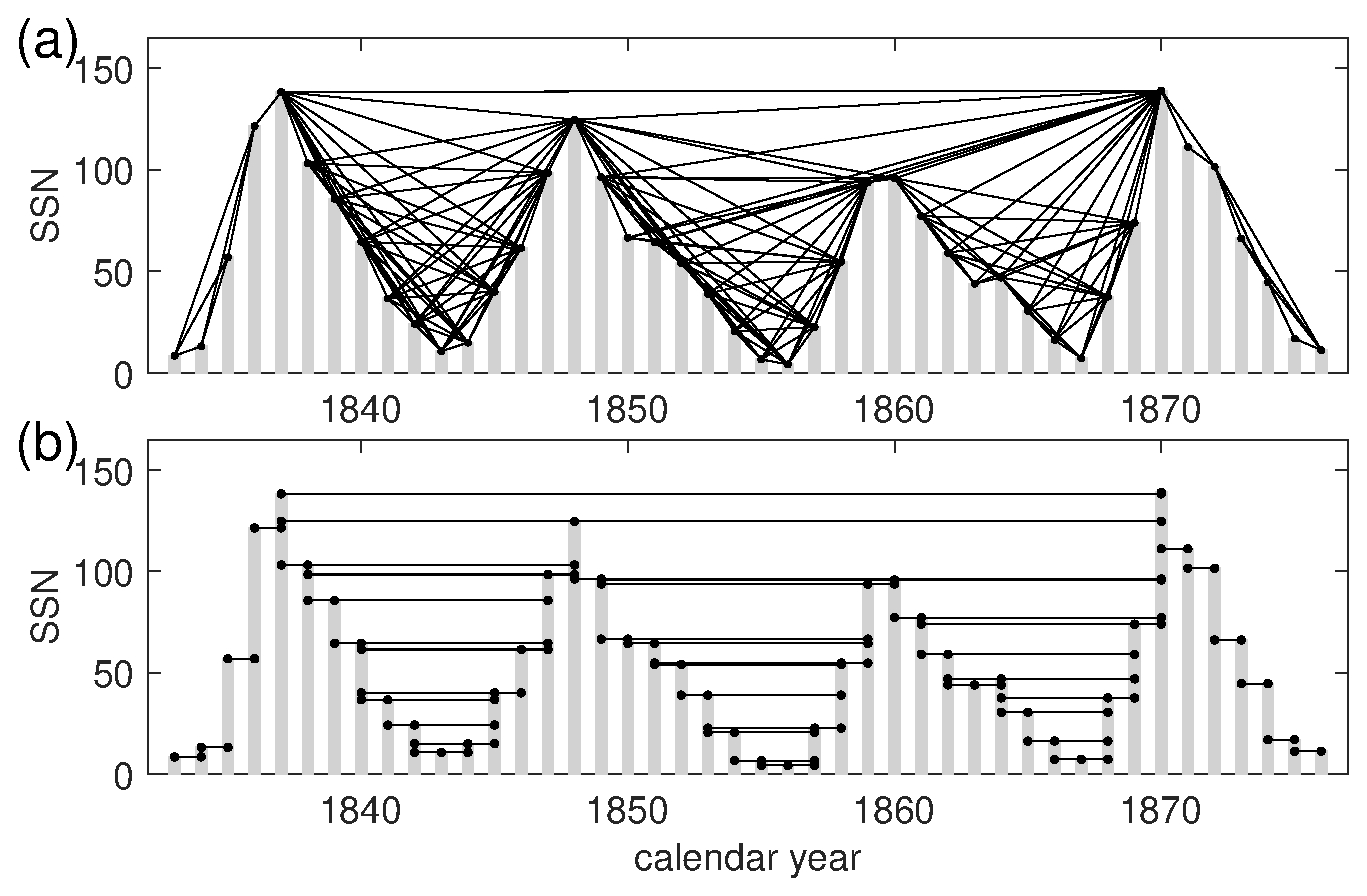
\includegraphics[width=\columnwidth]{Chapter04_VisibilityGt/TSspotnumberYear.eps}
			  \caption{Algorithm of constructing visibility graphs. \label{fig_chap04:timeseriesSS}}
			\end{figure}

also add recent aspects like binary VGs, other variants of VGs, fast estimation algorithms ($N\log N$), etc. here

	\subsection{Visibility graph properties}
		\subsubsection{Degree distributions}
		relationship with Hurst exponent in fractal / multifractal time series
		\subsubsection{Stochastic vs. deterministic dynamics}
		\subsubsection{Local network properties}
		\subsubsection{Global network properties}
		\subsubsection{Properties related to edge lengths}
		\subsubsection{Finite-sample effects}

influence of noise, missing values, time-scale uncertainty

also discuss here VGs for (marked) point processes like application to
earthquakes (Telesca et al.), draw link to natural time analysis method here???   

Maybe that's more like a separate subsection on "practical considerations",
together with noise effects, etc.

General question: What information can be gained from VGs? Which networks
properties are (when) useful to study? 

	\subsection{Bivariate visibility graph methods}
		\subsubsection{Visibility graph similarity}
		\subsubsection{Joint and excess degrees}


	\subsection{Decomposition of visibility graphs}
		\subsubsection{Time-directed visibility graphs}
		\subsubsection{Tests for time series irreversibility}
	\subsection{{\color{red} Identifying transitions by visibility graph method?
	Any references?}}


\section{Transition networks {\bf{(Reik)}} } \label{sec:TransitionNt}
The construction of the transition network depends on a proper phase space partition. For instance, we first mesh the phase space with box of equal sizes following the traditional idea of fractal dimension computations \cite{Grassberger1983PRL,Grassberger1983PLA} or complexity measures \cite{Crutchfield1989}. Then each partition is labeled with $\pi_i$ and regarded as a vertex in the network. The connectivity between partition $\pi_i$ and $\pi_j$ is then represented by the transition frequency following the temporal order of observations. Alternatively, one may define a partition as a ``state" based on a symbolic representation of time series, for instance, ordinal patterns of the series \cite{Li2008,McCullough2015}. Transforming the time series into a transition network is a process of mapping the temporal informaiton into a Markov chain to obtain a compressed or simplified representation of the original dynamics. 

	\subsection{Markov chains}
	In the terminology of Markov chain modeling \cite{Nicolis2005}, these partition algorithms generally map time series data to a Markov chain by defining nodes as some set of states that span the time series points, and allocating directed edges based on temporal succession that represent transitional probabilities based on the source data. Therefore, indicators of dynamics are derived from the transition matrix \cite{Nicolis2005}. 
	
	\subsection{Symbolic encoding of time series}
	Coarse-graining the range of values in a time series into a suitable set of classes (``symbols") $\{\pi_1, \dots , \pi_k \}$ allows considering the transition probabilities $w_{\alpha,\beta} = p (x_{i+1} \in \pi_\beta | x_i \in \pi_\alpha)$ between these classes in terms of a weighted and directed network. Therefore, the first step of this approach is to applying a suitable symbolic discretization to the phase space of the studied system. The next step is to explicitly use the temporal order of observations, i.e., their connectivity, to represent causality relationships contained in the dynamics of the observed dynamical system, which hence results in a time directed transition network. The directed network is represented by a weighted matrix $W = \{w_{\alpha, \beta} \}, \alpha, \beta \in [1, \cdots, k]$. Note that for a trajectory that does not leave a finite volume in phase space, there is only a finite number of discrete ``states" $\pi_i$ with a given minimum size in phase space. This implies the presence of absorbing or recurrent states in the resulting transition network. 
	
	The transition probability approach is well suited for identifying such ``states" (i.e. regions in phase space) that have a special importance for the causal evolution of the studied system in terms of betweenness centrality $b_v$ and related measures. Moreover, the resulting networks do not only depend on a single parameter, but on the specific definition of the full set of classes. Note, however, that coarse graining might be a valid approach in case of noisy real-world time series, where extraction of dynamically relevant information hidden by noise can be supported by grouping the data. In contrast to the other approaches for constructing complex networks from time series, the topology of transition networks depends on the specific choice of discretization. In the next sections, we give some examples.
		
		\subsubsection{Threshold-based coarse-graining}
		Note that meshing the phase space with equal size $\varepsilon$ is a threshold-based coarse-graining of the original system. Note that quantile mapping discretizing continuous time series shares much similarity with the threshold based coarse graining technique \cite{Liu2016}. In \cite{Donner2011}, we have illustrated an example in obtaining a transition network from time series of the Lorenz system. The transition behavior among different partitions is characterized by state transition matrix $W$, which is weighted and each entry $W_{ij}$ is estimated by the transition frequency from state $i$ to $j$. Traditionally, the transition entropy is simply the Shannon entropy of the weight matrix $W$, which is used to characterize the changes of the underlying system. 
		
		We note that the temporal information is lost after the coarse graining and the transition frequency matrix $W$ is estimated over the entire time series. Therefore, the resulting ordinal transition network is static representations \cite{Weng2017}. Inspired by the current ideas of temporal networks, Weng {\emph {et al.}} proposed to construct a temporal network from time series by unfolding temporal information $t$ into an additional topological dimension. More specifically, a transition from node $i$ to $j$ is established whenever the trajectory flow performs a transition from $i$ to $j$ at time $t$ which is denoted as ($i \to j; t$). By adding the additional time axis to the transition route, the consecutive memory network is constructed by introducing the memory factor $\tau$ and Weng {\textit{ et al.}} further proposed the memory entropy analysis to characterize the memory effect of the observed time series. The identified memory effect can accurately differentiate various types of time series including white noise, $1/f$ noise, AR model, periodic and chaotic time series. 
		
		\subsubsection{Order pattern-based coarse graining}
		There is a growing number of works in transforming time series into networks by ordinal partitions of time series \cite{Small2013,McCullough2015,Kulp2016b,McCullough2017b,Small2018}.  A series of systematic investigations of ordinal methods has been conducted in irregularly sampled time series \cite{Kulp2016a,McCullough2016,Sakellariou2016}, which shows high potential for studies of experimental observation data from climate sciences \cite{Eroglu2016}. In this method, the first step is to embed a one-dimensional time series $\{x(t)\}$ into phase space by using techniques from traditional time delay embedding, i.e., a proper choice of embedding dimension $D_x$ and time delay $\tau$. Then, embedded points in phase space are mapped to nodes in the network space according to its rank order and links are allocated between nodes based on temporal succession on the trajectory. In Fig. \ref{fig:rosTNm}, we show an example of ordinal partition network using the algorithms of \cite{McCullough2015}. 
\begin{figure}[ht]
	\centering
	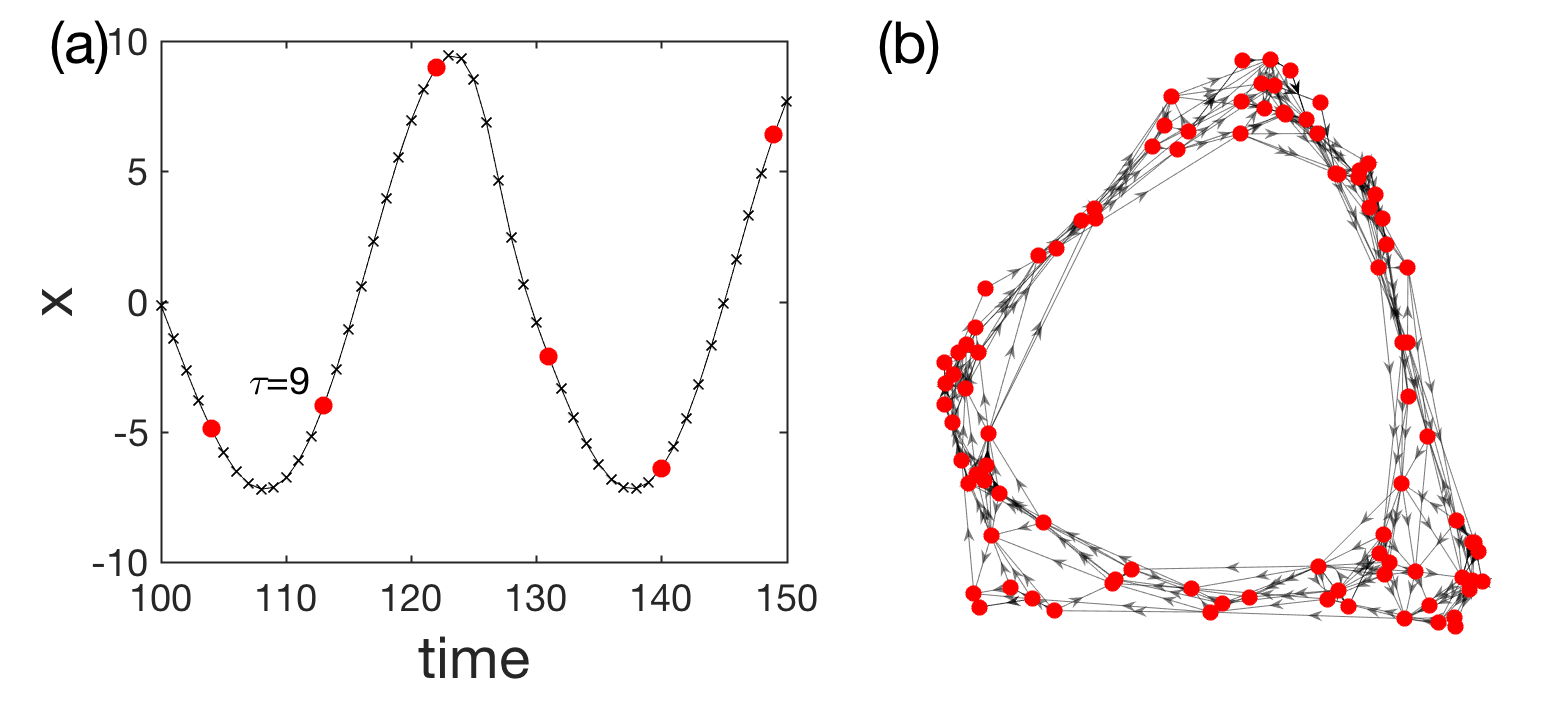
\includegraphics[width=\columnwidth]{Chapter05_TransitionNt/rosslerOPexample.eps}
\caption{(a) illustration of permutation symbols from a time series of the R\"ossler attractor ($a = 0.165$). Assume $\tau = 9$ and $D_x= 6$. The embedded vector is highlighted by red color $\vec{x}_{104} = \{x_{104}, x_{113}, x_{122}, x_{131}, x_{140}, x_{149} \}$ and its corresponding pattern is defined by the rank ordering $\pi_{104} = \{5, 1, 2, 4, 6, 3\}$. (b) ordinal pattern transition network (isolated vertices and self-loops are excluded for the visualization purpose). Directed edges are denoted by arrows. Reproduced from \cite{McCullough2015}. \label{fig:rosTNm}}
\end{figure}
		
		In \cite{McCullough2015}, McCullough {\textit{et al}} illustrated the construction algorithm in detail by the R\"ossler system and find that periodic dynamics translate to ring structures whereas chaotic time series translate to band or tube-like structures -- thereby indicating that this algorithm generates networks whose structure is sensitive to system dynamics. Furthermore, it is demonstrated that simple network measures including the mean out degree and variance of out degrees can track changes in the dynamical behaviour in a manner comparable to the largest Lyapunov exponent \cite{McCullough2015}. Therefore, these results show that measures of transition networks have the potential to be useful as indicators for dynamical discrimination and for detecting change points. 
		
		Note that the embedding dimension $D_x$ and time delay $\tau$ are two important parameters for constructing ordinal partition networks, in particular having crucial impacts on the appearance of forbidden order patterns \cite{Kulp2016b,McCullough2016,Sakellariou2016}. The selection of time delay $\tau$ must be chosen in relation to the sampling rate for continuous systems. The authors proposed using a time delay $\tau > 1$ \cite{Sun2014}. In \cite{McCullough2015}, they proposed to select these two parameters by traditional methods used for time series embedding, for instance, the first zero of the autocorrelation of the time series because it provides a sufficiently good phase space reconstruction for the R\"ossler time series. While there does not yet exist a robust metric for determining the correct choice of $D_x$, in the cases time series of the R\"ossler system they found that networks with the most visually intuitive structure often correspond with peak values of degree variance with respect to $D_x$. In addition, it was demonstrated that the range $6 \leq D_x \leq 10$ was the most useful when using simple network measures to track changes in dynamics \cite{McCullough2015}. Note that the choice of $D_x$ also determines the level of simplification of the original phase space by ordinal partitions. 
		
		Most of the recent works have focused only on univariate time series $\{x(t)\}$. However, the generalization to multivariate time series remains largely untouched. Most of the observable phenomena in the empirical sciences are of a multivariate nature. For instance, assets in stock markets are observed simultaneously and their joint development is analyzed to better understand tendencies. In climate science, multiple observations (temperature, pressure, precipitation, human activities etc, from different locations) are the basis of reliable predictions for the future climate conditions. 
		
		In \cite{Zhang2017b}, they propose to construct ordinal partition transition networks from multivariate (high dimensional) data. Given a scalar time series $\{x(t)\}$ which is produced by a deterministic dynamical system, the order structure of the time series depends on the embedding dimension $D_x$ and time delay $\tau$. Let us start with embedding dimension $D_x = 2$. Neglecting equality, we have two relations between $x(t)$ and $x(t + \tau)$, namely, two symbol sequences representing order patterns $\pi_{x}$:
\begin{equation} \label{piX2D_eq}
\pi_{x} (t) =  \begin{cases}
 1 & \text {if} \; x(t) < x(t + \tau), \\
 0 & \text {if} \; x(t) > x(t + \tau). 
\end{cases}
\end{equation}
In \cite{Small2013}, Small {\textit{et al}} used a fixed lag $\tau = 1$ for embedding and we follow this idea. By this choice, the order pattern $\pi_x^{1}$ captures the increasing trend, respectively, $\pi_x^{0}$ corresponds to the decreasing trend of the time series. This definition is equivalent to considering the signs of the increments $\Delta x(t) = x(t+1) - x(t)$ by a first-order difference of the original series. 

		Generalizing the above idea to the case of three dimensional time series $(x(t), y(t), z(t))$, we first obtain the increment series $(\Delta x(t), \Delta y(t), \Delta z(t))$. Then the order patterns are defined by the combinations of signs of $\Delta x(t), \Delta y(t)$ and $\Delta z(t)$. In particular, the ordinal pattern $\Pi(t) \in (\pi_1, \cdots, \pi_i), i = 1, \cdots, 8$ of a three dimensional time series $(x(t), y(t), z(t))$ is enumerated in Tab. \ref{tab:3D}. 
\begin{table}
\centering
\begin{tabular}{|c|c|c|c|c|c|c|c|c|}
\hline
$\Pi$      & $\pi_1$ & $\pi_2$ & $\pi_3$ & $\pi_4$ & $\pi_5$ & $\pi_6$ & $\pi_7$
& $\pi_8$\\
\hline
$\Delta x$ & $\pi_x^{1}, + $ & $\pi_x^{1}, + $ & $\pi_x^{1}, +$ &
$\pi_x^{1}, +$ & $\pi_x^{0}, - $ & $\pi_x^{0}, - $ &
$\pi_x^{0}, -$ & $\pi_x^{0}, -$\\
\hline
$\Delta y$ & $\pi_y^{1}, + $ & $\pi_y^{1}, + $ & $\pi_y^{0}, -$ &
$\pi_y^{0}, -$ & $\pi_y^{1}, + $ & $\pi_y^{1}, + $ &
$\pi_y^{0}, -$ & $\pi_y^{0}, -$\\
\hline
$\Delta z$ & $\pi_z^{1}, + $ & $\pi_z^{0}, - $ & $\pi_z^{1}, +$ &
$\pi_z^{0}, -$ & $\pi_z^{1}, + $ & $\pi_z^{0}, - $ &
$\pi_z^{1}, +$ & $\pi_z^{0}, -$\\
\hline
\end{tabular}
\caption{Order patterns in three dimensional time series $(x(t), y(t), z(t))$. 
\label{tab:3D}}
\end{table}
Therefore, the dimension of order pattern $\Pi(t)$ for an $n$-dimensional time series $(\{x_1\}(t), \ldots, \{x_n\}(t))$ is $D = 2^{n}$ since each component has either increasing or decreasing trend at time $t$. 

		Noting that we consider the increments between two consecutive time points of each measurement in the space of multi measurements, which captures the dynamic properties of the multi-variate time series in its associated velocity space (difference space). Therefore, time delay $\tau$ in the order pattern definition (Eq. \eqref{piX2D_eq}) has rather a different interpretation with the time delay that is often used in embedding. We can certainly generalize the discussion to the case of time delays larger than 1 (i.e., $\tau > 1$) and embedding dimension $D_x  > 2$ for each variable (measurement), but we think that the physical meaning in terms of dynamics becomes ambiguous for multivariate time series.  

		In addition, the resulting ordinal pattern transition network utilizes nullclines to obtain phase space partitions of the systems. As shown in Fig. \ref{fig:rosslerTwoA}(a), the chaotic R\"ossler system is color coded by the ordinal pattern partitions and the corresponding transition network in shown in Fig. \ref{fig:rosslerTwoA}b. 
\begin{figure}[ht]
	\centering
	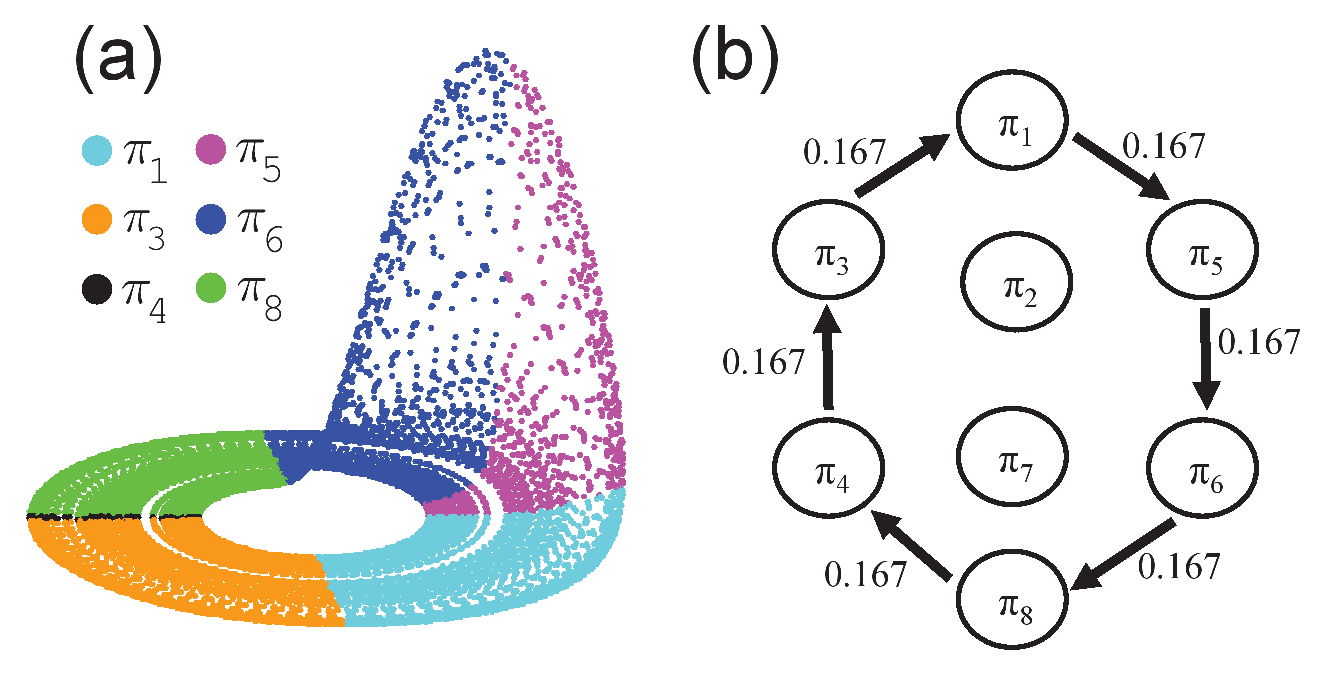
\includegraphics[width=0.7\columnwidth]{Chapter05_TransitionNt/rossler_0165N.eps}

\caption{(a) R\"ossler attractor in phase space color coded by order patterns ($a = 0.165$), (b) ordinal pattern transition network (self-loops are excluded). \label{fig:rosslerTwoA}}
\end{figure}

		In order to emphasize the importance of non-self transitions between ordinal patterns, we remove the self-loops, which is typical of most research work on complex networks \cite{Costa2007}. Furthermore, we remove self-loops before computing the weighted matrix $W$ to keep the normalization $\sum_{i,j}^{2^n} w_{ij} = 1$. Note that self-loops should not be expected with large amounts in stochastic processes. 
		
		Given the observations that different occurrence frequencies of ordinal patterns $p(\pi_i)$ and their transitions $w_{i,j}$, two Shannon entropies are defined as 
		\begin{align} \label{eq:Ho}
		\mathcal{H}_O &= - \sum_{i=1}^{2^n} p(\pi_i) \log_2 p(\pi_i) , \\ \label{eq:Ht}
		\mathcal{H}_T &= - \sum_{i,j=1}^{2^{n}} w_{ij} \log_2 w_{ij}. 
		\end{align}
		In the terminologies of \cite{McCullough2017b}, $\mathcal{H}_{O}$ characterizes the vertext (node) complexity and $\mathcal{H}_{T}$ is for the edge (link) transitional complexity, both of which have been shown useful for characterizing synchronization transition dynamics \cite{Zhang2017b}. Note that Eq. \eqref{eq:Ht} measures the transitional complexity of the ordinal patterns, but in a slightly different way of normalizations as used in \cite{McCullough2017b,Small2018}. 

		\subsubsection{Cross and joint ordinal transition networks} 
		The method of \cite{Zhang2017b} has been further generalized to construct cross and joint ordinal partition transition networks for two coupled systems \cite{Guo2018}. Let us start with an example of a single chaotic R\"ossler system as represented by three variables $(x_1(t), y_1(t), z_1(t))$. The ordinal pattern transition network is reconstructed based on the signs of the increments of each each variables $(\Delta x_1(t), \Delta y_1(t), \Delta z_1(t))$, where $\Delta x_1(t) = x_1(t+1) - x_1(t)$, $\Delta y_1(t) = y_1(t+1) - y_1(t)$, and $\Delta z_1(t) = z_1(t+1) - z_1(t)$. The definition of patterns $\Pi(t) \in (\pi_1, \cdots, \pi_i), i = 1, \cdots, 8$ are enumerated in Tab. \ref{tab:3D}. For two coupled systems, we have further time series from the other system as represented by $(x_2(t), y_2(t), z_2(t))$. 
		
		A cross ordinal pattern transition network (COPT) compares the relative speeds between two systems by the signs of $(\Delta x_1(t) - \Delta x_2(t)), (\Delta y_1(t) - \Delta y_2(t))$ and $(\Delta z_1(t) - \Delta z_2(t))$. The pattern definitions of a COPT are shown in Tab. \ref{tab:3DCOPT}. An example of COPT is reconstructed for two coupled R\"ossler system in a non-sync regime \cite{Guo2018}, which is shown in Fig. \ref{fig:rosCOPT}(a). 
\begin{table}[htb]
\centering
\begin{tabular}{|c|c|c|c|c|c|c|c|c|}
\hline
$\Pi$      & $\pi_1$ & $\pi_2$ & $\pi_3$ & $\pi_4$ & $\pi_5$ & $\pi_6$ & $\pi_7$
& $\pi_8$\\
\hline
$\Delta x_1 - \Delta x_2$ & $+ $ & $+ $ & $+$ & $+$ & $ - $ & $ - $ & $-$ & $ - $\\
\hline
$\Delta y_1 - \Delta y_2$ & $ + $ & $ + $ & $ -$ & $ -$ & $ + $ & $ + $ & $ -$ & $ -$\\
\hline
$\Delta z_1 - \Delta z_2$ & $ + $ & $ - $ & $ +$ & $ -$ & $ + $ & $ - $ & $+$ & $ -$\\
\hline
\end{tabular}
\caption{Pattern definitions of a COPT. Note that $``+"$ means a positive value while $``-"$ is for a negative value.  \label{tab:3DCOPT}}
\end{table}
Considering the effects of the different magnitudes of the three variables, we also compute an {\emph{alternative}} COPT by replacing $\Delta x_1(t) - \Delta x_2(t)$ by $\Delta x_1(t) / x_1(t) - \Delta x_2(t) / x_2(t)$, respectively, $\Delta y_1(t) - \Delta y_2(t)$ by $\Delta y_1(t) / y_1(t) - \Delta y_2(t) / y_2(t)$, and $\Delta z_1(t) - \Delta z_2(t)$ by $\Delta z_1(t) / z_1(t) - \Delta z_2(t) / z_2(t)$. An example of the alternative COPT is shown in Fig. \ref{fig:rosCOPT}(b). Comparing Fig. \ref{fig:rosCOPT}(a) to \ref{fig:rosCOPT}(b), the alternative COPT reflects better the non-coherent transitions between ordinal patterns since the coupling strength is in the non-synchronization regime ($\kappa_{1} = 0$ and $\kappa_{2} = 0.01$). 

\begin{figure}
	\centering
	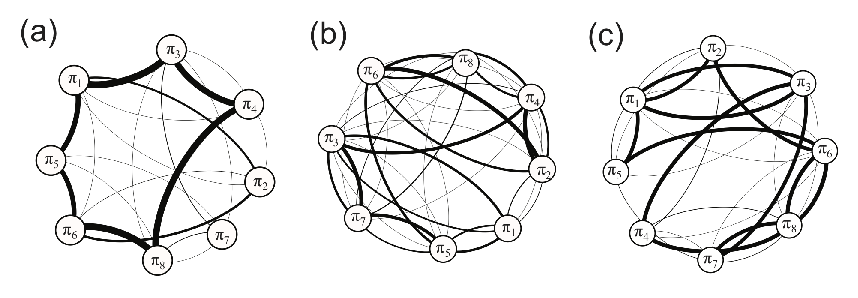
\includegraphics[width=\columnwidth]{Chapter05_TransitionNt/copt_jopt.eps}
	\caption{\small{Cross and joint ordinal pattern transition networks, which are reconstructed from two coupled R\"ossler systems in the non-sync regime \cite{Guo2018}. (a) Cross ordinal pattern transition network (COPT), (b) an alternative version of COPT, and (c) joint ordinal pattern transition network (JOPT). The directions of links have been suppressed for better visualizations. Reproduced from \cite{Guo2018}. } \label{fig:rosCOPT}}
\end{figure}	

		In an analogy, a joint ordinal pattern transition networks (JOPT) compares the relative speeds between two systems by the signs of $\Delta x_1(t) \cdot \Delta x_2(t), \Delta y_1(t) \cdot \Delta y_2(t)$ and $\Delta z_1(t) \cdot \Delta z_2(t)$ and the pattern definitions of a JOPT are summarized in Tab. \ref{tab:3DJOPT}. An example of JOPT is shown in Fig. \ref{fig:rosCOPT}(c).
\begin{table}[htb]
\centering
\begin{tabular}{|c|c|c|c|c|c|c|c|c|}
\hline
$\Pi$      & $\pi_1$ & $\pi_2$ & $\pi_3$ & $\pi_4$ & $\pi_5$ & $\pi_6$ & $\pi_7$
& $\pi_8$\\
\hline
$\Delta x_1 \cdot \Delta x_2$ & $+ $ & $+ $ & $+$ & $+$ & $ - $ & $ - $ & $-$ & $ - $\\
\hline
$\Delta y_1 \cdot \Delta y_2$ & $ + $ & $ + $ & $ -$ & $ -$ & $ + $ & $ + $ & $ -$ & $ -$\\
\hline
$\Delta z_1 \cdot \Delta z_2$ & $ + $ & $ - $ & $ +$ & $ -$ & $ + $ & $ - $ & $+$ & $ -$\\
\hline
\end{tabular}
\caption{Pattern definitions of a JOPT. Note that $``+"$ means a positive value while $``-"$ is for a negative value.  \label{tab:3DJOPT}}
\end{table}
In contrast to cross ordinal patterns, we notice that the joint ordinal patterns represent whether the respective variables of two systems show the same trend of changes or not, regardless of the magnitudes of the respective variables.

		The ideas of both COPT and JOPT have been particularly applied to analyze synchronization transitions \cite{Guo2018}. Note that a COPT and JOPT are two slightly different ways to construct networks from multivariate time series, providing complementary information. The ordinal patterns of a COPT are defined by considering the signs of the difference of $\Delta \vec{x}_1 - \Delta \vec{x}_2$ between two subsystems. In contrast, the ordinal patterns of a JOPT  are defined by the signs of the product of $\Delta \vec{x}_1 \cdot \Delta \vec{x}_2$. It is certain that the amplitudes of oscillations of different variables influence directly the definition of a COPT. However amplitudes become not important for a JOPT because only the signs of the product are considered. In addition, it is straightforward to generalize the ideas of JOPTs from two to three (or even $n$) coupled subsystems with an extended number of pattern definitions. However, it remains to be a big challenge for constructing a COPT for three coupled subsystems. 

		\subsubsection{Other approaches}
		For one dimensional symbol sequence, one may construct a directed symbol transition network \cite{Emmert2012}. Working with experimental data of $RR$-intervals from cardiac regulations, Makowiec {\textit{ et. al}} proposed to construct transitions networks from the subsequent increment series $\Delta RR_n = RR_n - RR_{n-1}$ \cite{Makowiec2013,Makowiec2013b,Makowiec2014b,Makowiec2015,Makowiec2015b,Makowiec2016}. In this series of work, they have demonstrated that transition network approaches are a powerful tool in quantifying the unique properties of the $RR$-interval time series of patients after heart transplant surgery. 
		
		When constructing ordinal partition transition networks by a sliding window scheme \cite{Small2013}, the ordinal pattern of the windowed sequence corresponds to one node of the network. Since the amplitude information is neglected, this approach may be combined with a transition network, where the nodes of the network are the binned amplitudes of the time series \cite{Sun2014}. More specifically, each time step $n$ is associated with a symbol-pair containing the amplitude information $\alpha (n)$ and the ordinal pattern $\pi (n)$. The former is calculated by binning the time series in the interval $[\min(\{ y_n\}), \max(\{ y_n \})]$ into $Q$ equal regions.  $\alpha(n)$ is then simply the bin number of $y_n$. Respectively, $\pi(n)$ is the ordinal pattern of the embedded vector $[y_n, y_{n+\tau}, \dots, y_{n+(L-1)\tau}]$. The symbol-pair at step $n$, $(\alpha(n), \pi(n))$, is then one node of the network and it is the connected by a directed link to the symbol-pair $(\alpha(n+1), \pi(n+1))$ of the successive time step. Furthermore, this algorithm has been combined with recurrence networks and surrogate networks, which has shown power in detecting weak nonlinearities in time series \cite{Laut2016}. 
		
		Coarse graining a financial time series, one may focus on the particular up-down behaviour of the volatility stock index series as presented in \cite{Li2006b,Li2007a}. More specifically, they symbolize time series by the parameter $\theta = \arctan \Delta x / \Delta t$, which characterizes the local increasing/decreasing velocity of the measurement. Then, the local velocities are coarse grained into four states ($R, r, d, D$), which correspond to violent-up meta, common-up meta, common down meta, and violent down meta patterns respectively. They found that the topological important nodes of the resulting transition networks play important roles in both information control and transport of stock market \cite{Li2007a}. 
		
		In a series of works by Gao \textit{et al.}\cite{Gao2014a,Gao2014,Gao2015}, they proposed a linear regression patterns transmission algorithm which captures the evolution of linear regression of bivariate time series. This algorithm has been demonstrated to be a useful tool to show the correlation mode transmission in crude oil spot price and future price \cite{Huang2015}. Based on reduced autoregressive models generated from time series, a proper directed transition network reconstruction algorithm has been proposed in \cite{Nakamura2012a}, such that the delay information has been successively captured by the transition behavior of the resulting network. Furthermore, proper surrogate method is required when extending these ideas from a univariate to multivariate time series analysis \cite{Nakamura2016}. 
		
		
	\subsection{Network interpretation of Markov chains}


\section{Other approaches {\bf{(Reik+Yong+All)}}}

Which other approaches should be mentioned here???

\section{Real-world applications {\bf{(All)}}}
	\subsection{Recurrence networks}
		\subsubsection{Example I: palaeoclimate data}
		\subsubsection{Example II: soil water }

	\subsection{Visibility graphs}
		\subsubsection{Example I: sunspot numbers}
		\subsubsection{Example II: Asymmetry of sunspots}

	\subsection{Transition networks}
	\subsection{Other approaches}

	\subsection{{\color{red} Please suggest any examples you may find
	appropriately here. Later, we will agree upon 1 or 2 examples which will
	discussed in detail for each method and mention briefly about other examples.
	We will include those examples that have been fully done to avoid futher
	serious calculations. } }



\section{Software implementation -- \texttt{pyunicorn} {\bf{(Jonathan+Norbert)}}}\label{sec:Software}
	In this chapter, we introduce the Python software package \texttt{pyunicorn}, which implements methods from both complex network theory and nonlinear time series analysis, and unites these approaches in a performant, modular and flexible way \cite{Donges2015}. Here, we mainly present a brief introduction of \texttt{pyunicorn} and a discussion of software structure and related computational issues. More details of the illustrative examples have been presented in \cite{Donges2015}.  Although in the tutorial of \cite{Donges2015}, the work flow of using \texttt{pyunicorn} is mainly illustrated drawing upon examples from climatology, the package is applicable to all fields of study where the analysis of (big) time series data is of interest, e.g. neuroscience \cite{Bullmore2009,Subramaniyam2014,Subramaniyam2015}. 
	
	\texttt{pyunicorn} is intended as an integrated container for a host of conceptionally related methods which have been developed and applied by the involved research groups for many years. Its aim is to establish a shared infrastructure for scientific data analysis by  means of complex networks and nonlinear time series analysis and it has greatly taken advantage from the backflow contributed by users all over the world. The code base has been fully open sourced under the BSD 3-Clause license.

	\texttt{pyunicorn}'s capabilities for analyzing and modeling complex networks are described including general networks, spatial networks, networks of interacting networks or multiplex networks and node-weighted networks. More specifically, {\color{red}as shown in Fig. shows the software architecture of \texttt{pyunicorn} displayed as a Unified Modeling Language (UML) diagram of class relationships.} \texttt{pyunicorn} presents methods for constructing and analyzing functional networks from fields of multiple time series, including cases demonstrating the application of climate network and coupled climate network analysis, methods for performing nonlinear time series analysis using recurrence plots, recurrence networks and visibility graphs. \texttt{pyunicorn} also presents methods for generating surrogate time series, which are useful for both functional network and network-based time series analysis. 
	
\begin{table*}[bth]
\caption{Structure of the \texttt{pyunicorn} software package listing the most important classes belonging to each submodule (selection for brevity).}
\begin{center}
\resizebox{\columnwidth}{!}{%
\begin{tabular}{lllll}
\hline
\textbf{core} & \textbf{funcnet} & \textbf{climate} & \textbf{timeseries} & \textbf{utils} \\
\hline
%(Sect.~\ref{sec:networks}) & (Sect.~\ref{sec:functional_networks}) & (Sects.~\ref{sec:climate_networks}, \ref{sec:coupled_climate_nets}) & (Sects.~\ref{sec:time_series}, \ref{sec:surrogates}) & (Sect.~\ref{sec:intro}) \\
\texttt{Network} & \texttt{CouplingAnalysis} & \texttt{ClimateNetwork} & \texttt{RecurrencePlot} & \texttt{mpi} \\
\texttt{GeoNetwork} & \texttt{CouplingAnalysisPurePython} & \texttt{CoupledClimateNetwork} & \texttt{CrossRecurrencePlot} & \texttt{navigator} \\
\texttt{InteractingNetworks} & & \texttt{TsonisClimateNetwork} & \texttt{JointRecurrencePlot} & \\
\texttt{ResNetwork} & & \texttt{SpearmanClimateNetwork} & \texttt{RecurrenceNetwork} & \\
\texttt{Data} & & \texttt{MutualInfoClimateNetwork} & \texttt{InterSystemRecurrenceNetwork} & \\
\texttt{Grid} & & \texttt{ClimateData} & \texttt{JointRecurrenceNetwork} & \\
 & & & \texttt{VisibilityGraph} & \\
 & & & \texttt{Surrogates} & \\
\hline
\end{tabular}
}
\end{center}
\label{tab:pyunicorn_structure}
\end{table*}%

The \texttt{pyunicorn} library is fully object-oriented and its inheritance and composition hierarchy reflects the relationships between the analysis methods. It consists of five subpackages (Tab.~\ref{tab:pyunicorn_structure}):
\begin{enumerate}
\item[\bf{core}] This name space contains the basic building blocks for general network analysis and modeling and is accessible after calling \texttt{import pyunicorn} %(Sect.~\ref{sec:networks}). 
The backbone \texttt{Network} class provides numerous standard and advanced complex network statistics, measures and generative models as well as import and export capabilities to GraphML, GML, NCOL, LGL, DOT, DIMACS and other formats. \texttt{Grid} and \texttt{GeoNetwork} extend these functionalities with respect to spatio-temporally embedded networks, which can be imported from and exported to ASCII and NetCDF files via the \texttt{Data} class. \texttt{InteractingNetworks} provides advanced methods designed for networks of networks (or multiplex networks), while \texttt{ResNetwork} specializes in power grids transporting electric currents and related infrastructure networks.

\item[\bf{funcnet}] Advanced tools for construction and analysis of general (non-climate) functional networks will be accommodated here. So far, \texttt{CouplingAnalysis} calculates cross-correlation, mutual information, mutual sorting information and their respective surrogates for large arrays of scalar time series.% (Sect.~\ref{sec:functional_networks}).

\item[\bf{climate}] Building on top of \texttt{GeoNetwork} and \texttt{Data}, the \texttt{ClimateNetwork} class and its children facilitate the construction and analysis of functional networks representing the statistical interdependency structure within a field of time series, based on similarity measures such as lagged linear Pearson or Spearman correlation and mutual information. %(Sect.~\ref{sec:climate_networks}). 
\texttt{CoupledClimateNetwork} extends this capability to the study of interrelationships between two distinct fields of observables.% (Sect.~\ref{sec:coupled_climate_nets}).

\item[\bf{timeseries}] This subpackage provides various tools for the analysis of non-linear dynamical systems and uni- and multivariate time series.% (Sect.~\ref{sec:time_series}). 
Apart from visibility graphs with time-directed measures (\texttt{VisibilityGraph} class), the focus lies on recurrence-based methods derived from the \texttt{RecurrencePlot} class. These include single, joint and cross-recurrence plots as well as standard, joint and inter-system recurrence networks, supporting time-delay embedding and several phase space metrics and are equipped with common measures of recurrence quantification analysis. \texttt{Surrogates} allow testing for the statistical significance of similarity measures by generating surrogate data sets under miscellaneous constraints from observable time series. %(Sect.~\ref{sec:surrogates}).

\item[\bf{utils}] Currently this includes \texttt{MPI} parallelization support and an experimental interactive network navigator.
\end{enumerate}

\texttt{pyunicorn} is conveniently applicable to research domains in science and society as different as neuroscience, infrastructure and climatology. Most computationally demanding algorithms are implemented in fast compiled languages on sparse data structures, allowing the performant analysis of large networks and time series data sets. The software's modular and object-oriented architecture enables the flexible and parsimonious combination of data structures, methods and algorithms from different fields. For example, combining complex network theory (\texttt{core.Network} class) and recurrence plots (\texttt{timeseries.RecurrencePlot} class) yields recurrence network analysis (\texttt{timeseries.RecurrenceNetwork} class), a versatile framework that opens new perspectives for nonlinear time series analysis and the study of complex dynamical systems in phase space. Another example are climate networks (\texttt{climate.ClimateNetwork} class), an approach bringing together ideas and concepts from complex network theory and classical eigen analysis of climatological data (e.g. empirical orthogonal function analysis) \cite{Donges2015}.

Along these lines, \texttt{pyunicorn} has the potential to facilitate future methodological developments in the fields of network theory, time series analysis and complex systems science by synthesizing existing elements and by adding new methods and classes that interact with or build upon preexisting ones. Nonetheless, we urge users of the software to ensure that such developments are theoretically well-founded and explicable as well as motivated by well-posed and relevant research questions to produce high-quality research.

Besides \texttt{pyunicorn}, we suggest that some other software packages are available, for instance, the MATLAB toolbox CRPtool that allows to get the adjacency matrix (or recurrence matrix). Furthermore, this toobox provides the computation of several network measures like clustering coefficients $\mathcal{C}$ and transitivity $\mathcal{T}$. In addition, we recommend some network visualization toolboxes, including Gephi or Networkx which can be used to analyze the networks (when the recurrence matrix is available).



\section{Conclusions and future perspectives {\bf{(All)}}} \label{sec:Discussion}
	\subsection{Conclusions and discussion}
Comments by Jonathan:

- What is the added value of network methods compared to standard methods?

- Why do network methods typically seem to work better with small data sets than standard methods? Does this have to do with $N^2$ of information units (although not independent) being created from N data points through building an adjacency matrix, leading to more robust statistics?

- What are common applications of network methods? Such as identifying regime shifts / transitions / tipping points in time series, distinguishing different dynamical regimes, analysis of dynamical system structure in phase space, prediction of some types... What more?

We might probably start with taking these points already in the introduction (as motivating questions beyond the methodological interest) and take them up for more detailed discussion at the end of the review.

For recurrence network approaches, there are some evident questions, the most relevant being about the invariance of findings under variation of the threshold value $\varepsilon$ since this value determines the link density of the network and all network characteristics become trivial in the limit of full connectivity \cite{Bradley2015c}.

	\subsection{Future perspectives}
	Some of the following topics should be paid for more attention, which are currently under investigations. Furthermore, the questions as discussed in the previous sections should be integrated into the following working packages. 
	\begin{enumerate}
		\item Evolving network analysis for time series remains largely open, for instance, by temporal network approaches. 

	There is one natural extension of network science from static to dynamic analysis, which build models by evolving networks that change as a function of time. The generalization to evolving network analysis for time series remains largely open, which however almost all real world networks evolve over time, either by adding or removing nodes or links over time. Evolving network concepts build on established network theory and are now being introduced into studying networks in many diverse fields \cite{Holme2012}. Taking social networks as examples, people make and lose friends over time, thereby creating and destroying edges, and some people become part of new social networks or leave their networks, changing the nodes in the network. 


	The most common way of characterizing evolving networks is to treat evolving networks as successive snapshots of a static network. In analyzing time series, we often use running (sliding) window technique and network analysis is performed for each window. This set of all individual static windows compose a motion perspective over time. Dynamical changes or regime shifts are then tracked by the variations of network properties. Unfortunately, the sliding window technique to a motion picture also reveals the main difficulty with this approach, namely, empirical choices of time window lengths and the window overlapping which are rarely suggested by the network analysis. Using extremely small window sizes between two consecutive snapshot preserves resolution, but may actually obscure wider trends which only become visible over longer timescales. Conversely, using larger window sizes loses the temporal order of events within each snapshot. Therefore, we need careful choices of the appropriate timescale for dividing the evolution of a network into static snapshots, which have certain effects on proper interpretations of the results \cite{Donges2011,Zou2014}. 

	Anyway, such a sliding window technique does not cover all aspects of the temporal structures of networks \cite{Holme2012}. More generally, we need to include an additional time dimension to quantify the detailed information on the temporal sequences of the network structures, for instance, timings when the edges are active or not. The time ordering have important effects that can not be captured by static networks, especially when considering dynamical processes on top of networks. When coming to time series analysis, Weng {\textit{et al}} \cite{Weng2017} proposed to transform time series into temporal networks by encoding temporal information into an additional topological dimension of the graph, which captures the ``lifetime" of edges. We note that a proper combination of ordinal pattern transition network approach (for instance, short-term transition networks) may provide the temporal information for this problem since the transition matrix describes the probability of future evolution directions of the trajectory in phase space. 

		\item Multilayer and multiplex network analysis for multiple time scale time series. 

	In this work, we have provided a review on the existing methods in reconstructing multilayer and multiplex networks from time series, for instance, multiplex recurrence networks, multiplex visibility graphs, inter-system cross recurrence networks, and joint recurrence networks etc. However, most of these methods are appropriate for stationary time series as we have discussed in Sec. \ref{subsec:practicalRN}. When monitoring complex physical systems over time, one often finds multiple phenomena in the data that work on different time scales. For example, observations are collected on a smaller time scale, and also exhibit time series behavior over a larger time scale, which is rather typical for data of climate sciences. Another prominent example from neuroscience is the recording of spiking activity of individual neurons (discrete event series) and local field potentials (time continuous measurement). Variability of the data on the smaller scale can obscure the time series behavior of the data on the larger scale, making it more difficult to identify the larger scale trends. If one is interested in analyzing and modeling these individual phenomena, it is crucial to recognize the multiple time scales in the construction of multilayer and multiplex networks from time series.  


		\item Bringing complex network methods to understanding complexity from various disciplines. 

	In future, we need to demonstrate the existing methods by more applications to various disciplines, particularly providing deeper insights to the existing knowledge of the respective topics. Depending on the particular working topic, it is crucial to make good use of the network analysis to extract some features that are not easily captured by most of the standard methods. 


		\item The inverse problem of regeneration of time series from networks. 

	Most of the existing works focus on the proper transformation methods mapping a time series into network representations. However, regeneration of time series from a network as denoted by the adjacency matrix is remains a big challenge, which certainly has many applications. In networks, the order of the vertices can be exchanged without affecting the network topology. But for this reconstruction of the trajectory the temporal order of the nodes is required. Depending on different network representations for time series, regeneration algorithms should be different. Recently these methods have been focused on mainly on recurrences \cite{thiel2004b,hirata2008,Hirata2016}, $k$ nearest neighbor networks \cite{Hou2015,Khor2016}, and ordinal transition networks \cite{McCullough2017}. For all these different algorithms, there are several important algorithmic parameters that have to be chosen empirically in order to guarantee consistent topology between the reconstructed time series and the original system. The computational complexity of each algorithm has to be evaluated in the future work. One application of such regeneration algorithms is to perform surrogate analysis, for example, to test the statistical significance of the results obtained for the original time series. Therefore, we have to take into account the proper choice of null hypothesis while proposing algorithms regenerating time series from networks. 


		\item Building network models for time series prediction. 

	Time series modeling and forecasting has attracted a great number of researchers' attention, which is the core of nonlinear time series analysis \cite{kantz1997,Bradley2015c}. To this end, we build a proper model to forecast the system's future behavior, given a sequence of observations of one or a few time variable characteristics. Most of methods originated from nonlinear dynamics are state-space models, which build local model in 'patches' of a reconstructed state space and then use that model to make the prediction of the next point, which remains an active area of research \cite{Bradley2015c}. In the case of stochastic processes, delay vector strategies have been further proposed to generalize the state-space models to short-term prediction. We note that most of existing network approaches to nonlinear time series analysis have been focusing on characterizing network features of phase space. Time series modeling and prediction have not been reported in the literature yet.  

	\end{enumerate}



\section{Summary {\bf{(All)}}}



\section*{Acknowledgements}


\bibliography{references}




\end{document}
